\documentclass{article}
\usepackage{graphicx} % Required for inserting images
\usepackage{amssymb} % For \leftrightarrow
\usepackage{amsmath}
\usepackage{hyperref}
\newcommand{\E}{\mathbb{E}}
\usepackage{listings}
\usepackage{xcolor}

\lstset{
    language=Python,
    basicstyle=\ttfamily\small,
    keywordstyle=\color{blue},
    commentstyle=\color{gray},
    stringstyle=\color{orange},
    numbers=left,
    numberstyle=\tiny\color{gray},
    breaklines=true,
    frame=lines
}


\title{BachelorThesis}
\author{Fran Tomazic}
\date{March 2026}

\begin{document}

\maketitle

\section{Introduction}

The problem of estimating species richness, which is the total number of distinct species present in an assemblage, including those not observed in any sample, has a long history across multiple disciplines. The 1943 paper by Fisher, Corbet and Williams~\cite{fisher1943} laid the mathematical foundation for statistical approaches to this problem. Around the same time, Good and Turing developed frequency estimation methods as part of their effort to crack German ciphers during World War II~\cite{good1953,good2000}. Since then the ``species problem'' has appeared in ecology (estimating butterfly species on an island), biology (counting microbial taxa), genetics (enumerating alleles), software engineering (finding undiscovered bugs), and linguistics (determining how many words an author knew)~\cite{chao2016species}.

In nearly all of these settings, counting the true richness is almost impossible. A sample will almost always miss a fraction of the true existing species, and the simple count of observed species $S_{\mathrm{obs}}$ systematically underestimates the true richness $S$. The magnitude of this negative bias depends on the heterogeneity of the underlying abundance distribution: the more unequal the species abundances, the more rare species the sample will fail to detect. This makes the gap between $S_{\mathrm{obs}}$ and $S$ the central statistical challenge of the field.

\vspace{1em}

Our main question throughout this paper is: \emph{how can we estimate the total spoken vocabulary of a person from a finite recording of their speech?} In this setting, each distinct word corresponds to a species and each token (word occurrence) corresponds to an individual. Later on we will define more precisely what we mean by a distinct word. Spoken vocabulary falls right into the regime where species richness estimation is most difficult: word frequencies are highly heterogeneous, governed by the Zipf's law, which states that the frequency of a word is approximately inversely proportional to its rank~\cite{baayen2001}.What is the rank in this context? Suppose you order all the words of a text by their frequencies, then the highest frequency word has rank 1, second highest has rank 2, etc... By the formula we get that $f(1)\propto{1}$ and $f(2)\propto{1/2}$ thus the rank 1 word appears twice as often as the rank 2 word.  A small number of words (\emph{the}, \emph{is}, \emph{a} \emph{and}) represent a large share of all tokens, while the majority of distinct words appear only once or twice in any finite sample. Therefore, the number of words observed exactly once or twice, commonly referred to as singletons and doubletons, is always large, and the fraction of the vocabulary that remains unseen is substantial even in lengthy recordings.

A person's \emph{active} spoken vocabulary (with how many different words they speak on a daily basis) is considerably smaller than their \emph{passive} vocabulary (the words they can understand). Research in applied linguistics suggests that comprehension of spoken texts requires knowledge of roughly 6\,000 to 7\,000 word families, whereas written texts require 8\,000 to 9\,000. But what a person \emph{produces} in conversation is a much smaller, context-dependent subset of even their active vocabulary. Estimating the size of this active vocabulary from a finite speech sample is therefore a nontrivial statistical problem, and one that is well suited to the tools of nonparametric species richness estimation. We will also compare estimates derived from spoken data with those from written text, where we expect greater lexical diversity due to the wider range of registers and the time available for word choice.

\vspace{1em}

In this thesis we proceed as follows. In Section~\ref{sec:framework} we establish the mathematical framework and notation for species richness estimation, distinguishing abundance data from incidence data and defining sample coverage. Section~\ref{sec:estimators} reviews the classical nonparametric estimators such as Good-Turing, Chao1, iChao1, ACE, and the jackknife, discussing the assumptions, strengths, and limitations of each. Section~\ref{sec:shape} presents the main theoretical contribution: shape-constrained estimation via $k$-monotone and completely monotone distributions, We explain why using the completely monotone model is a natural next step when the degree of monotonicity $k$ is large.
Section~\ref{sec:data} describes our data sources: the Shakespeare word counts from Spevack~\cite{Spevack1968} for replication, and our own spoken language corpus for the novel analysis. Section~\ref{sec:results} presents the results, including estimator comparisons, rarefaction and extrapolation curves. We discuss the findings in Section~\ref{sec:discussion} and conclude in Section~\ref{sec:conclusion}.


\section{Framework and Notation}\label{sec:framework}

Let us define our framework and notation. Consider an assemblage consisting of $N$ total individuals, which is a finite set, each belonging to one of $S$ distinct species. Let $N_i$ denote the number of individuals of the $i^{th}$ species in the assemblage, with $i = 1, 2, \ldots, S$ and $N_i > 0$. The total population size is
\[
    N = \sum_{i=1}^{S} N_i\,.
\]
The relative abundance of species $i$ is $p_i = N_i / N$, with 
$\sum_{i=1}^{S} p_i = 1$. The quantities $N$, $S$, $N_i$, and $p_i$ 
represent the true and unknown parameters of the assemblage.

Assume we draw a random sample of $n$ individuals from the assemblage, thus having\quad $n<N$.\quad In this sample, a total of $S_{\mathrm{obs}}$ distinct species are observed, we call it the \emph{reference sample}. Let $X_i$ be the number of individuals of the $i^{th}$ species observed in this sample. Only species with $X_i > 0$ are observable, and $\sum_{i=1}^{S} X_i = n$. We denote by $f_k$ the \emph{abundance frequency count}: the number of species represented by exactly $k$ individuals in the reference sample, for $k = 1, 2, \ldots, n$. That is,
\[
    f_k = \#\{i : X_i = k\}\,.
\]
The sample size can then be expressed in terms of the abundance frequency counts as
\[
    n = \sum_{i=1}^{S} X_i = \sum_{k \geq 1} k\, f_k\,.
\]

We call $f_1$ the number of \emph{singletons} (species observed exactly once) and $f_2$ the number of \emph{doubletons} (species observed exactly twice). Singletons and doubletons play a central role in many estimation methods, as we will see in Section~\ref{sec:estimators}. More generally, most of the information about the undetected species is contained in the lower-order frequency counts $f_1, f_2, \ldots, f_r$ for small $r$. The quantity we wish to estimate is $f_0$: the number of species present in the assemblage but absent from the reference sample. The true species richness decomposes as

\begin{equation}\label{eq:fundamental}
    S = S_{\mathrm{obs}} + f_0\,.
\end{equation}

Since $S_{\mathrm{obs}}$ is directly observed, the entire estimation 
problem reduces to estimating $f_0$.

\subsection{Sampling data structures}
 
There are two principal types of sampling data: abundance data and incidence data.

\paragraph{Abundance data.}
In abundance sampling, the sampling unit is an individual. In the discrete-type variant, a fixed number $n$ of individuals is drawn from a study area. In the continuous-type variant, sampling effort is measured on a continuous scale such as time, area, or volume. For our application, we record a speaker for a fixed period of time, and each word said constitutes an individual drawn from the speaker's vocabulary. The resulting data are discrete-type abundance data.


\paragraph{Incidence data.}
In incidence sampling, the sampling unit is not an individual but a spatial or temporal unit (a quadrat, a time window, etc.). For each of $T$ sampling units, one records only the detection or non-detection of each species, yielding an incidence matrix $[W_{ij}]$ and incidence-based frequency counts $Q_k$ ($k = 1, \ldots, T$), the number of species detected in exactly $k$ sampling units. Therefore $Q_T$ refers to the number of species detected in all of the sampling units. The number of all observed species is given by $\sum_{k=1}^T Q_k$. Since our data consist of individual words with their frequencies, we work mostly with abundance data throughout this thesis. For a detailed treatment of incidence-based methods, we refer to Chao and Chiu~\cite{chao2016species}.


\subsection{Sample coverage}\label{subsec:coverage}
 
An important concept for assessing how complete a sample is, is the notion of \emph{sample coverage}. Introduced by Good and Turing~\cite{good1953}, it estimates the proportion of the total number of individuals in the assemblage that belong to species represented in the sample. Turing's estimator is
\begin{equation}\label{eq:coverage_turing}
    \hat{C} = 1 - \frac{f_1}{n}\,.
\end{equation}
Intuitively, $f_1/n$ estimates the probability that the next sampled individual belongs to a species not yet observed, subtracting it from 1 gives the coverage. A coverage close to 1 indicates that most of the assemblage's individuals belong to species already detected, whereas a low coverage signals that many species remain unobserved.


Chao and Jost~\cite{chaojost2012} proposed a bias-corrected version:
\begin{equation}\label{eq:coverage_chaojost}
    \hat{C} = 1 - \frac{f_1}{n} \cdot 
    \frac{(n-1)\,f_1}{(n-1)\,f_1 + 2\,f_2}\,.
\end{equation}


This adjustment reduces the bias of the basic Turing estimator, particularly when singletons dominate the sample (i.e.\ when $f_1$ is large relative to $n$). Sample coverage will play an important role later, both as a diagnostic for the completeness of our speech samples and as the basis for coverage-based standardization when comparing samples of different sizes.

\vspace{1em}

Figure~\ref{fig:sample_coverage_examples} illustrates the scale of the coverage values in concrete examples. 
A high value of \(\hat C\) indicates that most of the probability mass belongs to word types already seen in the sample. 
A lower value indicates that a substantial part of the vocabulary is still represented only through rare types, especially singletons.

\begin{figure}[ht]
    \centering
    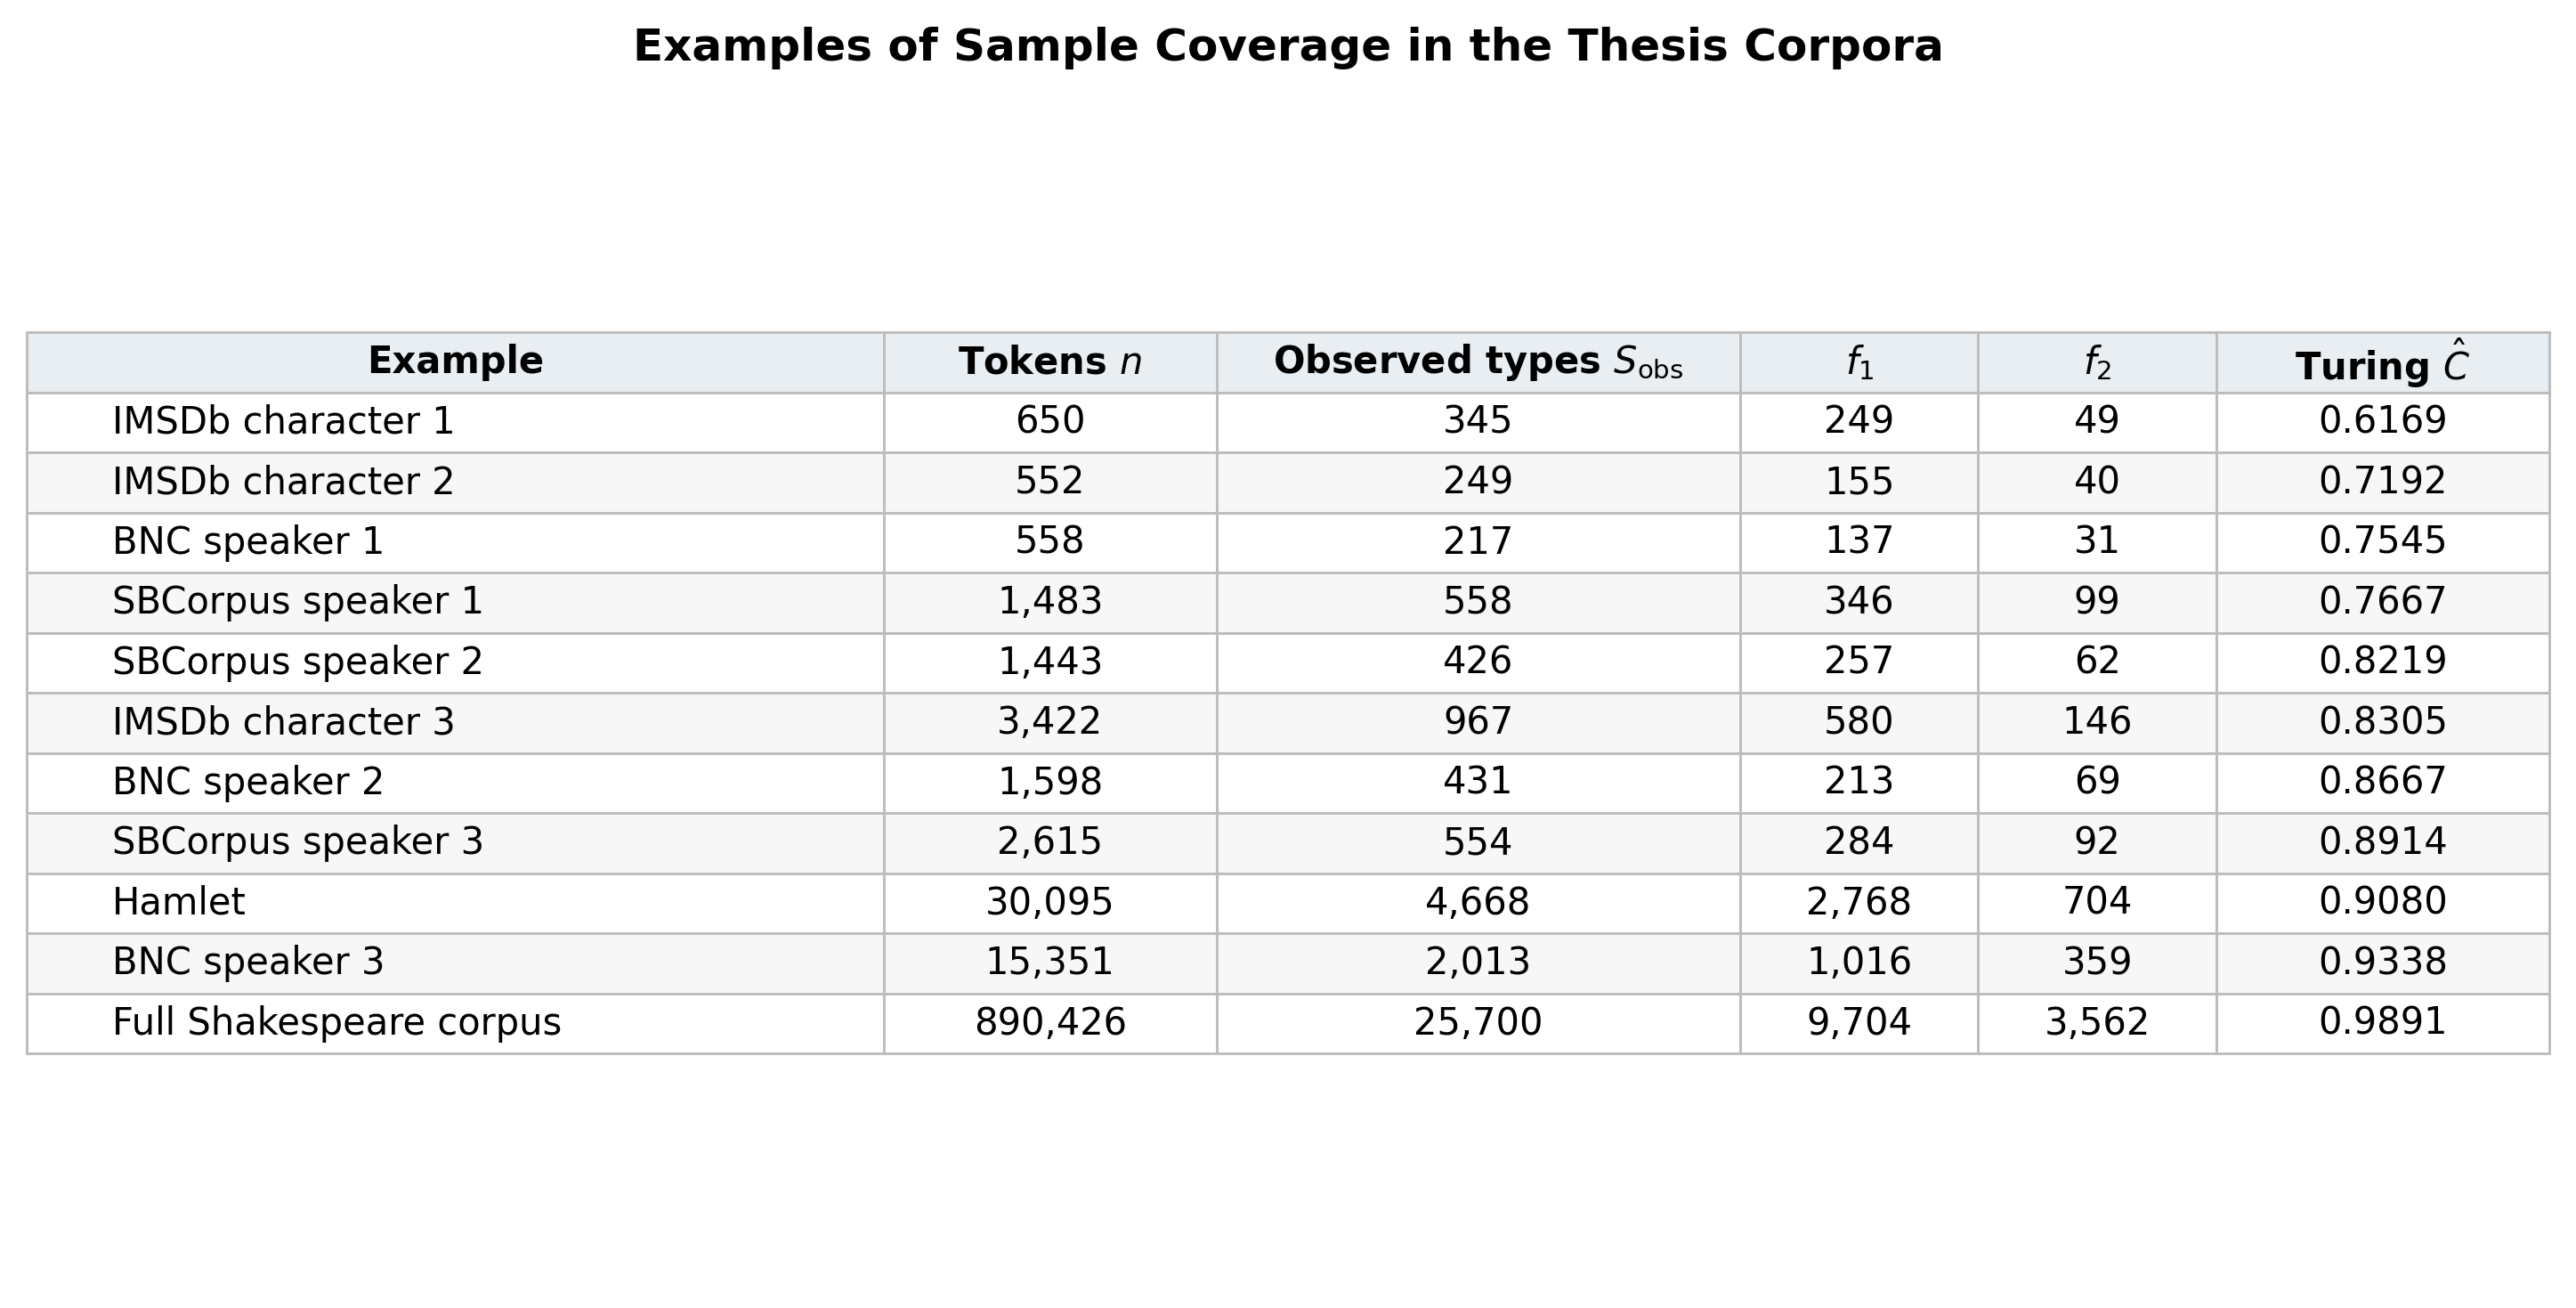
\includegraphics[width=\textwidth]{../code/intuition/sample_coverage_examples.png}
    \caption{Examples of Turing sample coverage for several texts and speakers used in this thesis.}
    \label{fig:sample_coverage_examples}
\end{figure}


\subsection{Parametric and nonparametric approaches}

A parametric model assumes that the species abundance distribution belongs to a known family of distributions, fully characterized by a finite parameter vector $\theta$. Common choices include the log-normal, the inverse-Gaussian, and the Zipf-Mandelbrot law. While such models can yield efficient estimators when the assumed form is well specified, simulations have shown that they perform poorly when it is not~\cite{chao2016species}. Moreover, two parametric models may fit the observed data equally well yet produce widely different estimates of $S$, making the choice of distributional family a source of considerable uncertainty (as illustrated in Figure~\ref{fig:mixture_models}).

A nonparametric model makes no assumption about the functional form of the underlying abundance distribution. Instead, the number of undetected species is estimated directly from the lower-order frequency counts $f_1, f_2, \ldots, f_r$ for some small $r$. This approach is more robust across applications and permits meaningful comparisons between assemblages, since it does not require that different assemblages follow the same distributional family. All the estimators considered in this thesis are nonparametric.

\subsection{Rarefaction, extrapolation, and standardization}

When comparing species richness across multiple assemblages (for example, the vocabulary of two different speakers, or spoken versus written language from the same individual), a direct comparison of $S_{\mathrm{obs}}$ is misleading if the sample sizes differ, since larger samples will generally detect more species. Two standardization approaches are commonly used.

 
\paragraph{Sample-size-based rarefaction and extrapolation.}
Rarefaction asks: if we had drawn only $m < n$ individuals, how many species would we expect to observe? By subsampling from the reference sample, one constructs a \emph{rarefaction curve} that shows expected richness as a function of the sample size. Conversely, extrapolation projects the curve beyond the observed sample size, predicting how many additional species would be detected if sampling effort were increased~\cite{chaojost2012}.

\vspace{1em}

Figure~\ref{fig:rarefaction_extrapolation_medium_example} shows why raw observed richness is not directly comparable across samples of different size. Even for a fixed text, the expected number of observed word types changes substantially with the number of sampled tokens. Rarefaction and extrapolation therefore provide a common sampling-effort scale on which different assemblages can be compared.

\begin{figure}[ht]
    \centering
    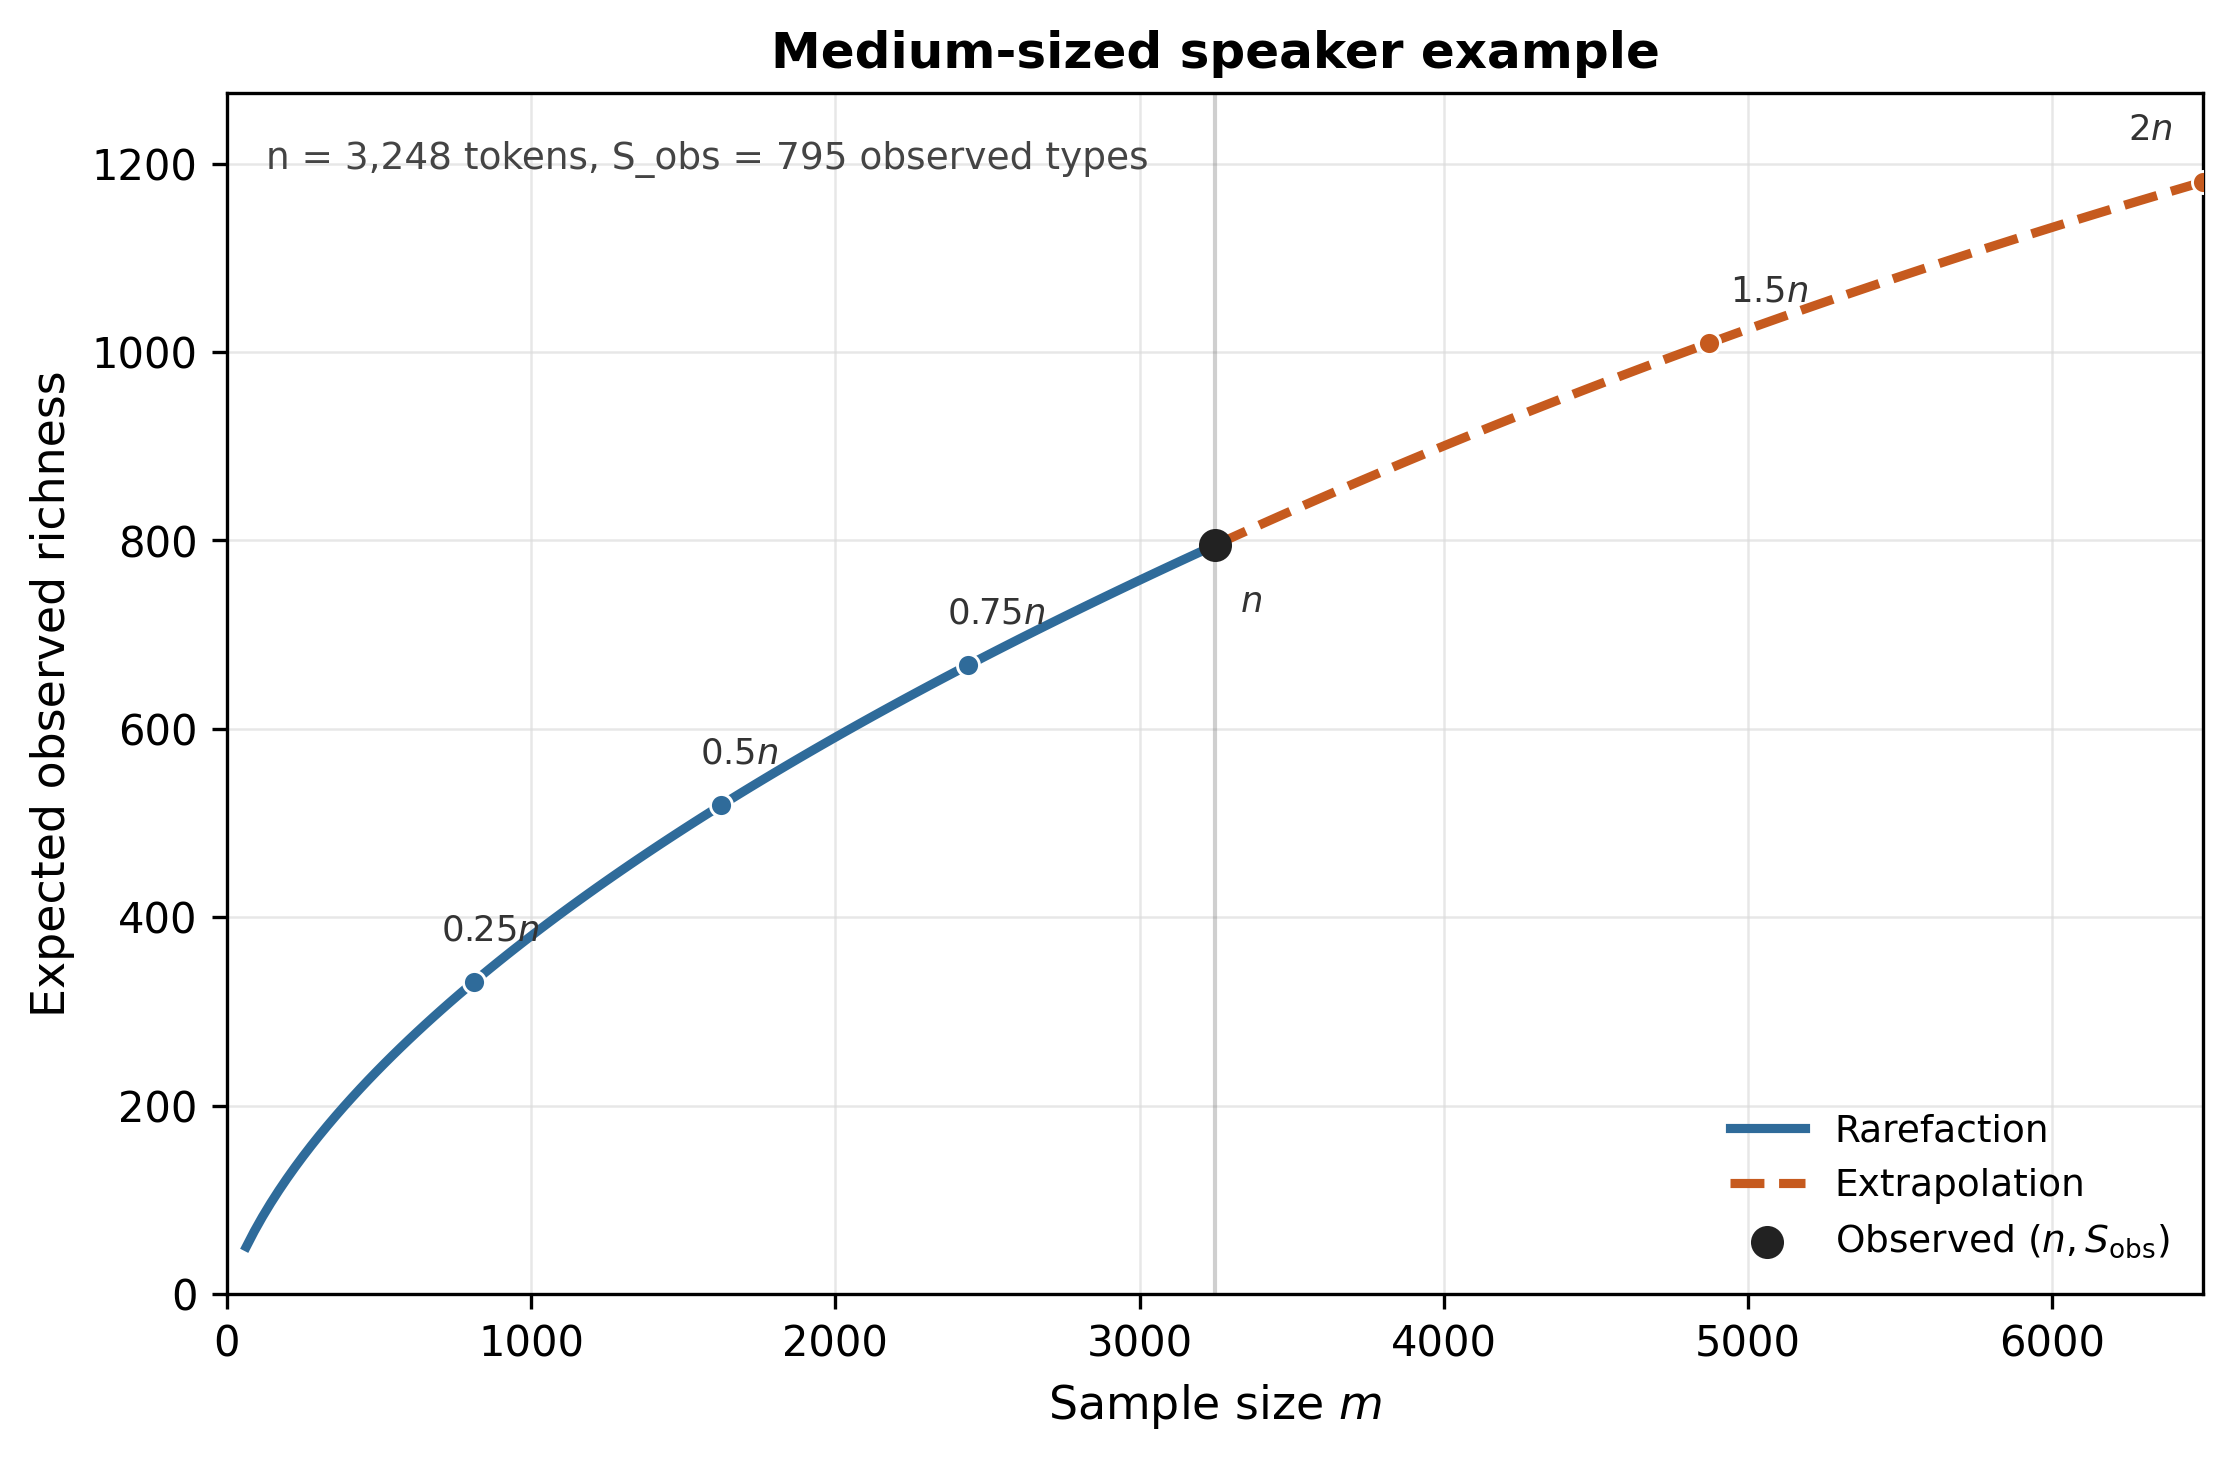
\includegraphics[width=\textwidth]{../code/intuition/rarefaction_extrapolation_medium_example.png}
    \caption{Sample-size-based rarefaction and extrapolation for one example text. The solid curve gives the expected observed richness for smaller sample sizes \(m<n\), the point marks the observed sample \((n,S_{\mathrm{obs}})\), and the dashed curve extrapolates richness up to twice the observed sample size.}
    \label{fig:rarefaction_extrapolation_medium_example}
\end{figure}
 
\paragraph{Coverage-based standardization.}
An alternative, proposed by Chao and Jost~\cite{chaojost2012}, standardizes samples not by size but by coverage. The rationale is that two samples of equal size may represent very different levels of completeness: a sample of $n = 5\,000$ tokens from a speaker with homogeneous word usage may achieve near-complete coverage, while the same $n$ from a speaker with a highly heterogeneous vocabulary may miss a substantial fraction of species. By comparing richness at equal coverage, one obtains a fairer comparison that accounts for the difficulty of each assemblage. We will use both approaches when comparing our spoken and written data in Section~\ref{sec:results}.


\section{Existing Nonparametric Estimators}\label{sec:estimators}

In this section we review the principal nonparametric estimators of species richness. All of them estimate the number of undetected species $f_0$ using only the lower-order frequency counts, without assuming any particular distributional form for the species abundances.


\subsection{Good--Turing frequency estimation}

The Good--Turing frequency estimator, developed by I.\,J.\ Good based on ideas from Alan Turing, originated in their wartime work on cracking German ciphers~\cite{good1953,good2000}. Good initially modelled the species frequencies using a multinomial distribution, but found this approach inaccurate for rare species. The key insight of Good--Turing estimation is to adjust the observed frequency of a species: for a species observed $k$ times, its estimated probability is
\begin{equation}
    \label{eq:good_turing}
    \hat{p}_k =
    \begin{cases}   
        \dfrac{(k+1)\,f_{k+1}}{n\,f_k}, & k > 0, \\[6pt]
        \dfrac{f_1}{n}, & k = 0.
    \end{cases}
\end{equation}
where $n$ is the total sample size.
$\hat{p}_0$ is \emph{not} the count of undetected species $f_0$; rather, it estimates the fraction of the assemblage's individuals that belong to species absent from the sample. It is the complement of the sample coverage $\hat{C} = 1 - f_1/n$ defined in 
Section~\ref{subsec:coverage}.

\paragraph{Simple Good--Turing smoothing.}
A practical difficulty with Equation~\eqref{eq:good_turing} is that for large $k$, the frequency counts $f_k$ become noisy and sparse, making the ratio $f_{k+1}/f_k$ unstable. The Simple Good--Turing (SGT) algorithm addresses this by replacing the raw counts with smoothed values $S(f_k)$ obtained from a log-linear regression of $\log f_k$ on 
$\log k$~\cite{gale1995}:
\begin{equation}\label{eq:sgt}
    p_k = \frac{(k+1) \cdot S(f_{k+1})}{n \cdot S(f_k)}\,.
\end{equation}
For small values of $k$, where the counts are reliable, one uses $S(f_k) = f_k$ directly, the smoothed values are used only in the sparse tail. We will not go into further detail on the regression procedure here, as the SGT algorithm is not the main focus of our analysis.


\subsection{Chao1-type estimators}

The Chao1 estimator, introduced by Chao~\cite{chao1984}, is the most widely used nonparametric lower bound for species richness. Its derivation applies the Cauchy-Schwarz inequality to the expected frequency counts, which guarantees that the result is a lower bound for $S$ regardless of the true abundance distribution.
Now we present the derivation.

\paragraph{Derivation.}
Assume each species $i$ has detection rate $\lambda_i$ drawn from some distribution $G$, and that conditional on $\lambda_i$, the species count follows a $\mathrm{Poisson(\lambda_i)}$ distribution (this framework is developed fully in Section~\ref{sec:mixture_models}). The expected frequency counts then satisfy:

\[
\E[f_j] = S \int_0^{\infty} \frac{\lambda^j\, e^{-\lambda}}{j!}\,
dG(\lambda)\,, \qquad j = 0, 1, 2, \ldots
\]
In particular,
\[
\begin{aligned}
\E[f_0] &= S \int_0^{\infty} e^{-\lambda}\, dG(\lambda), \\
\E[f_1] &= S \int_0^{\infty} \lambda e^{-\lambda}\, dG(\lambda), \\
\E[f_2] &= \frac{S}{2} \int_0^{\infty} \lambda^2 e^{-\lambda}\, dG(\lambda), \\
\E[f_3] &= \frac{S}{6} \int_0^{\infty} \lambda^3 e^{-\lambda}\, dG(\lambda).
\end{aligned}
\]
Define the probability measure
$dH(\lambda) = e^{-\lambda}\, dG(\lambda) \big/ \int e^{-\lambda}\,
dG(\lambda)$, so that the expectations can be rewritten as
\[
\E[f_1] = \E[f_0] \int_0^{\infty} \lambda\, dH(\lambda)\,,
\qquad
\E[f_2] = \frac{\E[f_0]}{2} \int_0^{\infty} \lambda^2\,
dH(\lambda)\,.
\]
By the Cauchy--Schwarz inequality,
$\bigl(\int \lambda\, dH\bigr)^2 \leq \int \lambda^2\, dH$, which
gives
\[
\bigl(\E[f_1]\bigr)^2 \leq 2\,\E[f_0]\,\E[f_2]\,.
\]
Rearranging yields a lower bound on the number of undetected species:
\begin{equation}\label{eq:chao1_bound}
\E[f_0] \geq \frac{\bigl(\E[f_1]\bigr)^2}{2\,\E[f_2]}\,.
\end{equation}
Replacing $\E[f_j]$ by the observed $f_j$ and adding $S_{\mathrm{obs}}$ gives the Chao1 estimator (with a finite-sample bias correction):
\begin{equation}\label{eq:chao1}
    \hat{S}_{\mathrm{Chao1}} =
    \begin{cases}
        S_{\mathrm{obs}} + \dfrac{n-1}{n} \cdot
        \dfrac{f_1^2}{2 f_2}\,,
            & \text{if } f_2 > 0\,, \\[8pt]
        S_{\mathrm{obs}} + \dfrac{n-1}{n} \cdot
        \dfrac{f_1 (f_1 - 1)}{2}\,,
            & \text{if } f_2 = 0\,.
    \end{cases}
\end{equation}


For large sample sizes $n$, the correction factor $(n-1)/n$ is negligible and the estimator simplifies to
$\hat{S}_{\mathrm{Chao1}} \approx S_{\mathrm{obs}} + f_1^2/(2f_2)$.

The Cauchy--Schwarz inequality is sharp: equality holds if and only if $\lambda$ is constant under $H$, i.e., all species have the same detection rate. This means the Chao1 estimator achieves the true value only in the homogeneous case where all species are equally detectable. In practice, this condition is rarely met for linguistic data, where word frequencies are highly heterogeneous. When heterogeneity is high, the true $f_0$ can substantially exceed the Chao1 estimate, meaning the estimator underestimates the true richness~\cite{chao2016species,schmitz2025}.


\paragraph{The iChao1 estimator.}
Chiu et al.~\cite{chiu2014} derived an improved lower bound by extending the Cauchy-Schwarz argument to incorporate tripletons $f_3$ and quadrupletons $f_4$:
\begin{equation}\label{eq:ichao1}
    \hat{S}_{i\mathrm{Chao1}} =
    \hat{S}_{\mathrm{Chao1}} +
    \frac{n-3}{n} \cdot \frac{f_3}{4 f_4}
    \times
    \max\!\left(
        f_1 - \frac{n-3}{n-1} \cdot \frac{f_2 f_3}{2 f_4},\; 0
    \right).
\end{equation}
For large $n$, this simplifies to
$\hat{S}_{i\mathrm{Chao1}} \approx \hat{S}_{\mathrm{Chao1}} 
+ \frac{f_3}{4 f_4} \max\!\left(f_1 - \frac{f_2 f_3}{2 f_4},\, 0\right)$.
By incorporating higher-order frequency counts, iChao1 tightens the lower bound when there is additional information in $f_3$ and $f_4$ beyond what $f_1$ and $f_2$ alone provide.


\subsection{ACE-type estimators}

The Abundance-based Coverage Estimator (ACE), developed by Chao and Lee~\cite{chaolee1992}, extends the idea of sample coverage by incorporating a measure of heterogeneity among the rare species. The central idea is that abundant species are almost certain to appear in any sample and therefore carry no information about the undetected fraction $f_0$. Only the rare species, whose detection is uncertain, are informative. ACE formalizes this by splitting the observed species into two groups using a cutoff value $k$ (conventionally $k = 10$, following Chao and Lee~\cite{chaolee1992}):

\begin{align*}
    S_{\mathrm{abun}} &= \sum_{i > k} f_i\,,  &
    S_{\mathrm{rare}} &= \sum_{i=1}^{k} f_i\,, \\[4pt]
    n_{\mathrm{rare}} &= \sum_{i=1}^{k} i\, f_i\,,  &
    \hat{C}_{\mathrm{rare}} &= 1 - \frac{f_1}{n_{\mathrm{rare}}}\,,
\end{align*}
where $n_{\mathrm{rare}}$ is the sample size restricted to the rare group and $\hat{C}_{\mathrm{rare}}$ is Turing's coverage applied to that group.

The key quantity is the squared coefficient of variation (CV) of the species abundances:
\begin{equation}\label{eq:cv}
    \gamma^2 = \frac{S^{-1} \cdot \sum_{i=1}^{S} (p_i - \bar{p})^2}
    {\bar{p}^2}\,,
\end{equation}
where $\bar{p} = 1/S$. This characterizes the degree of heterogeneity among species abundances: $\gamma^2 = 0$ if and only if all species have equal abundances (homogeneous assemblage), and larger values of $\gamma^2$ indicate greater heterogeneity. The ACE estimator is then by:

\begin{equation}\label{eq:ace}
    \hat{S}_{\mathrm{ACE}} = S_{\mathrm{abun}} 
    + \frac{S_{\mathrm{rare}}}{\hat{C}_{\mathrm{rare}}} 
    + \frac{f_1}{\hat{C}_{\mathrm{rare}}} \cdot 
    \hat{\gamma}^2_{\mathrm{rare}}\,,
\end{equation}
with the estimated squared CV of the rare group given by
\begin{equation}\label{eq:cv_rare}
    \hat{\gamma}^2_{\mathrm{rare}} = \max\!\left\{
    \frac{S_{\mathrm{rare}}}{\hat{C}_{\mathrm{rare}}}
    \cdot
    \frac{\sum_{i=1}^{k} i(i-1)\, f_i}
    {\left(\sum_{i=1}^{k} i\, f_i\right)
     \left(\sum_{i=1}^{k} f_i - 1\right)}
    - 1,\; 0 \right\}.
\end{equation}

The cutoff $k = 10$ is conventional and simulation studies suggest that the estimator is reasonably robust to moderate changes in this value~\cite{chaolee1992}. However, for data with extremely heavy tails (as in linguistic applications), the choice of cutoff may have a larger effect and must be studied.

\subsection{Jackknife estimators}
The jackknife is a general-purpose technique for reducing the bias of an estimator~\cite{burnham1979}. The idea is as follows: from the reference sample of $n$ individuals, one systematically removes one individual at a time and recomputes the estimator on each reduced sample. The resulting \emph{pseudo-values} are then combined to produce a bias-corrected estimate. This is the first-order jackknife; the second-order version extends the procedure by considering pairs of removed individuals, yielding a more aggressive bias correction at the cost of higher variance.
 
The first-order jackknife estimator for species richness is
\begin{equation}\label{eq:jk1}
    \hat{S}_{jk1} = S_{\mathrm{obs}} + \frac{n-1}{n} \cdot f_1 
    \approx S_{\mathrm{obs}} + f_1\,,
\end{equation}
and the second-order jackknife estimator is
\begin{equation}\label{eq:jk2}
    \hat{S}_{jk2} = S_{\mathrm{obs}} + \frac{2n-3}{n} \cdot f_1 
    - \frac{(n-2)^2}{n(n-1)} \cdot f_2 
    \approx S_{\mathrm{obs}} + 2f_1 - f_2\,.
\end{equation}
 
The first-order jackknife adds approximately $f_1$ to 
$S_{\mathrm{obs}}$, effectively assuming that every singleton represents one missed species, this was initially the idea of Turing. Its a rough correction that tends to underestimate the true richness when the sample is small (because many species are missed entirely and do not even appear as singletons) and to overestimate when the sample is large (because some singletons are genuinely rare species that would not yield additional undetected species). The second-order jackknife partially addresses this by subtracting a term proportional to $f_2$, which tempers the correction when doubletons are numerous~\cite{burnham1979}.

\subsection{Summary and limitations}
 
Each of the estimators above has characteristic strengths and weaknesses. Good--Turing provides the conceptual foundation (sample coverage and the probability mass of unseen species) but does not directly yield an estimate of $f_0$ as a count. Chao1 gives a guaranteed lower bound that is easy to compute and widely applicable, but it can severely underestimate the true richness when species abundances are highly heterogeneous, precisely the situation we face with word frequency data. iChao1 tightens the bound by incorporating $f_3$ and $f_4$, but remains a lower bound. ACE accounts for heterogeneity through the coefficient of variation, but depends on the choice of cutoff $k$. The jackknife estimators offer bias reduction but lack the theoretical guarantee of a lower bound and can overshoot.
 
A common limitation shared by all of these methods is that they use  only the first few frequency counts and treat the rest of the abundance distribution as a black box. In the next section, we explore a fundamentally different approach: instead of extracting information from a handful of frequency counts, we impose a \emph{shape constraint} on the entire distribution of abundances. This leads to the $k$-monotone and completely monotone estimators, which can exploit more of the available information while still remaining nonparametric.

\section{Beyond Frequency-Count Estimators}\label{sec:shape}

\subsection{Nonparametric mixture models}\label{sec:mixture_models}

The estimators presented in Section~\ref{sec:estimators} rely on only the first few frequency counts $f_1, f_2, \ldots, f_r$ for small $r$, discarding the rest of the observed abundance distribution. Mixture models take a different approach: they model the \emph{entire} distribution of species abundances, using all available data to estimate the probability $p(0;G)$ that a species goes undetected. Nonparametric mixture models are particularly attractive because they make no assumption about the shape of the underlying abundance distribution, relying only on the assumption that abundances are drawn from some common distribution.

\paragraph{The mixture framework.}
We begin by defining the mixture model framework. Suppose we have $N$ species, and each species $i$ has its own abundance parameter $\lambda_i$, which governs how frequently it appears in a sample. Since we cannot know all $N$ individual parameters, we assume that $\lambda_1, \lambda_2, \ldots, \lambda_N$ are independent draws from a common distribution $G$, called the \emph{mixing distribution}. The model then has two layers:
\begin{enumerate}
    \item \textbf{Conditional layer:} Given $\lambda_i$, the number of times species $i$ is observed in the sample follows some simple distribution, typically a $\mathrm{Poisson}(\lambda_i)$ distribution.
    \item \textbf{Mixing layer:} The parameters $\lambda_1, \ldots, \lambda_N$ are themselves random, drawn independently from $G$.
\end{enumerate}

\paragraph{The mixture distribution.}
Since each species has its own rate $\lambda_i$, and we never observe those rates directly (only the counts). To obtain the \emph{mixture distribution}: the probability that a randomly chosen species is observed exactly $x$ times in the sample, we need to average the Posson likelihood over all possible values of $\lambda$, weighted by how likely each value is under $G$. Concretely, the Poisson probability of observing $x$ occurrences given rate $\lambda$ is $\lambda^xe^{-\lambda}/x$. And multiplying this by $dG(\lambda)$ and integrating over all $\lambda>0$ gives the unconditional probability: 
\begin{equation}\label{eq:poisson_mixture}
    p(x; G) = \int_0^{\infty} \frac{\lambda^x \, e^{-\lambda}}{x!} 
    \, dG(\lambda)\,, \qquad x \in \mathbb{N}_0\,.
\end{equation}
This is no longer a Poisson distribution; it is a weighted average of Poisson distributions with different rates, where the weights come from $G$. When we set $x = 0$ it gives us the probability that a species is entirely missed in the sample:
\begin{equation}\label{eq:p0}
    p(0; G) = \int_0^{\infty} e^{-\lambda} \, dG(\lambda)\,.
\end{equation}
Once $p(0;G)$ is known, the total number of species can be estimated directly.

\vspace{1em}

The mixing distribution $G$ captures the heterogeneity among species abundances. Its shape determines how many species are rare versus common, which in turn determines $f_0$, the number of species missed by the sample. For spoken vocabulary data, this heterogeneity is extreme: a handful of function words (\emph{the}, \emph{is}, \emph{and}) dominate the token counts, while the vast majority of distinct words appear only once or twice.

\paragraph{Why Poisson sampling.}
The preceding section took the Poisson conditional model as given. We now justify this choice. The Poisson assumption arises naturally from the sampling setup. When recording a speaker for a fixed period of time, each specific word has a small probability of appearing at any given moment, but there are many opportunities for it to occur. This regime, where we have many independent opportunities combined with a small probability per opportunity, is precisely where the Poisson distribution applies. More precisely, the underlying model is binomial, and the Poisson arises as its limit when the number of opportunities grows large. We can derive this connection in two complementary settings: \emph{incidence data}, where the observation period is cut into time slots, and \emph{abundance data}, where time is treated as continuous.

\vspace{1em}
 
\subparagraph{Incidence data:}
Suppose we divide a recording of length $T$ into $n$ time slots. In each slot, a given word either appears or it does not. This means each slot is approximately an independent Bernoulli trial. Let $p$ denote the probability that the word fills any given slot and define $\lambda = np$ as the expected number of times the word is heard in the whole recording. The count $X$ of how many times the word appears then follows a binomial distribution:
\[
X \sim \mathrm{Binomial}(n,p), \qquad
\Pr(X=k) = \binom{n}{k}p^k(1-p)^{n-k}.
\]
Substituting $p = \lambda/n$, the probability mass function becomes
\[
\Pr(X=k) = \binom{n}{k}\left(\frac{\lambda}{n}\right)^k\left(1-\frac{\lambda}{n}\right)^{n-k}.
\]
We now take $n \to \infty$ with $\lambda$ and $k$ fixed. The combinatorial factor satisfies
\[
\binom{n}{k}\left(\frac{\lambda}{n}\right)^k
=
\frac{n(n-1)\cdots(n-k+1)}{k!}\,\frac{\lambda^k}{n^k}
=
\frac{\lambda^k}{k!}\left(1\right)\left(1-\frac{1}{n}\right)\cdots\left(1-\frac{k-1}{n}\right)
\;\longrightarrow\; \frac{\lambda^k}{k!}\,,\ as\ n\rightarrow\infty.
\]
For the remaining factor, the classical exponential limit gives
\[
\left(1-\frac{\lambda}{n}\right)^{n-k}
=
\left(1-\frac{\lambda}{n}\right)^{n}
\left(1-\frac{\lambda}{n}\right)^{-k}
\;\longrightarrow\; e^{-\lambda}\cdot 1
=
e^{-\lambda}\,,\ as\ n\rightarrow\infty
\]
since $n - k \approx n$ for large $n$. Combining the two limits yields
\[
\Pr(X=k)
\;\longrightarrow\;
\frac{\lambda^k\, e^{-\lambda}}{k!}\,,
\]
which is the Poisson probability mass function with parameter $\lambda$. Thus, for large $n$, the binomial model is well approximated by a Poisson distribution.

\subparagraph{abundance data:}
The same result can be obtained in a continuous-time framework. If we model the occurrences of each word as a Poisson process with rate $\lambda_i$\ (a counting process satisfying that the rate parameter $\lambda$ is constant over time, it's independent over non-overlapping intervals, and it is impossible to have simultaneous events), then the number of occurrences in an observation window of length $T$ follows a $\mathrm{Poisson}(\lambda_i T)$ distribution. The derivation proceeds via a system of ordinary differential equations solved by induction; see, e.g., Joyce~\cite{joyce2014poisson}. Since both routes lead to the same Poisson model, the choice between them is a modelling convenience: the discrete-slot view is more natural for a fixed-length corpus, while the continuous-time view arises naturally when the sampling effort is measured in time rather than token count.


\paragraph{Parametric versus nonparametric mixtures.}
If $G$ is assumed to belong to a known parametric family, the estimation problem reduces to fitting a small number of parameters. This can be efficient when the assumed family is correct, but different parametric models may fit the observed data equally well yet yield widely different estimates of $S$~\cite{chao2016species}. To illustrate this, we fit three standard two-parameter mixture models to the Shakespeare corpus:
\begin{itemize}
    \item the \emph{Gamma--Poisson} (negative binomial) mixture, where
          $\Lambda \sim \mathrm{Gamma}(r, r/\mu)$;
    \item the \emph{LogNormal--Poisson} mixture, where
          $\log\Lambda \sim \mathcal{N}(\mu, \sigma^2)$;
    \item the \emph{Poisson--Inverse Gaussian} mixture, where
          $\Lambda \sim \mathrm{InvGaussian}(\mu, \phi)$.
\end{itemize}
In each case, $X \mid \Lambda = \lambda \sim \mathrm{Poisson}(\lambda)$.
The full probability mass functions are given in Appendix~\ref{app:parametric_models}.

Figure~\ref{fig:mixture_models} compares the three fits. The left panel shows the observed region ($x \geq 1$): all three models capture the shape of the abundance distribution reasonably well, with the Poisson--Inverse Gaussian mixture providing the closest fit ($\chi^2 = 79.5$) and the Gamma--Poisson the worst ($\chi^2 = 8952.3$). However, the right panel reveals dramatic disagreement in the unobserved region. The Gamma--Poisson model assigns $p(0) = 0.974$, implying that nearly all species are undetected and yielding an estimate of $\hat{N} \approx 1{,}004{,}540$, roughly 40 times the observed vocabulary. The LogNormal--Poisson gives $\hat{N} \approx 36{,}788$, while the Poisson--Inverse Gaussian gives $\hat{N} \approx 57{,}903$. Three models, comparable fit to the observed data, and estimates of total vocabulary size spanning two orders of magnitude.

\vspace{1em}

This sensitivity to the parametric form of $G$ motivates the nonparametric approach: if $G$ is left completely unspecified, no distributional form is assumed, avoiding the risk of misspecification. This flexibility makes nonparametric mixtures particularly suited to problems like vocabulary estimation, where the true shape of the abundance distribution is unknown.

\begin{figure}[ht]
    \centering
    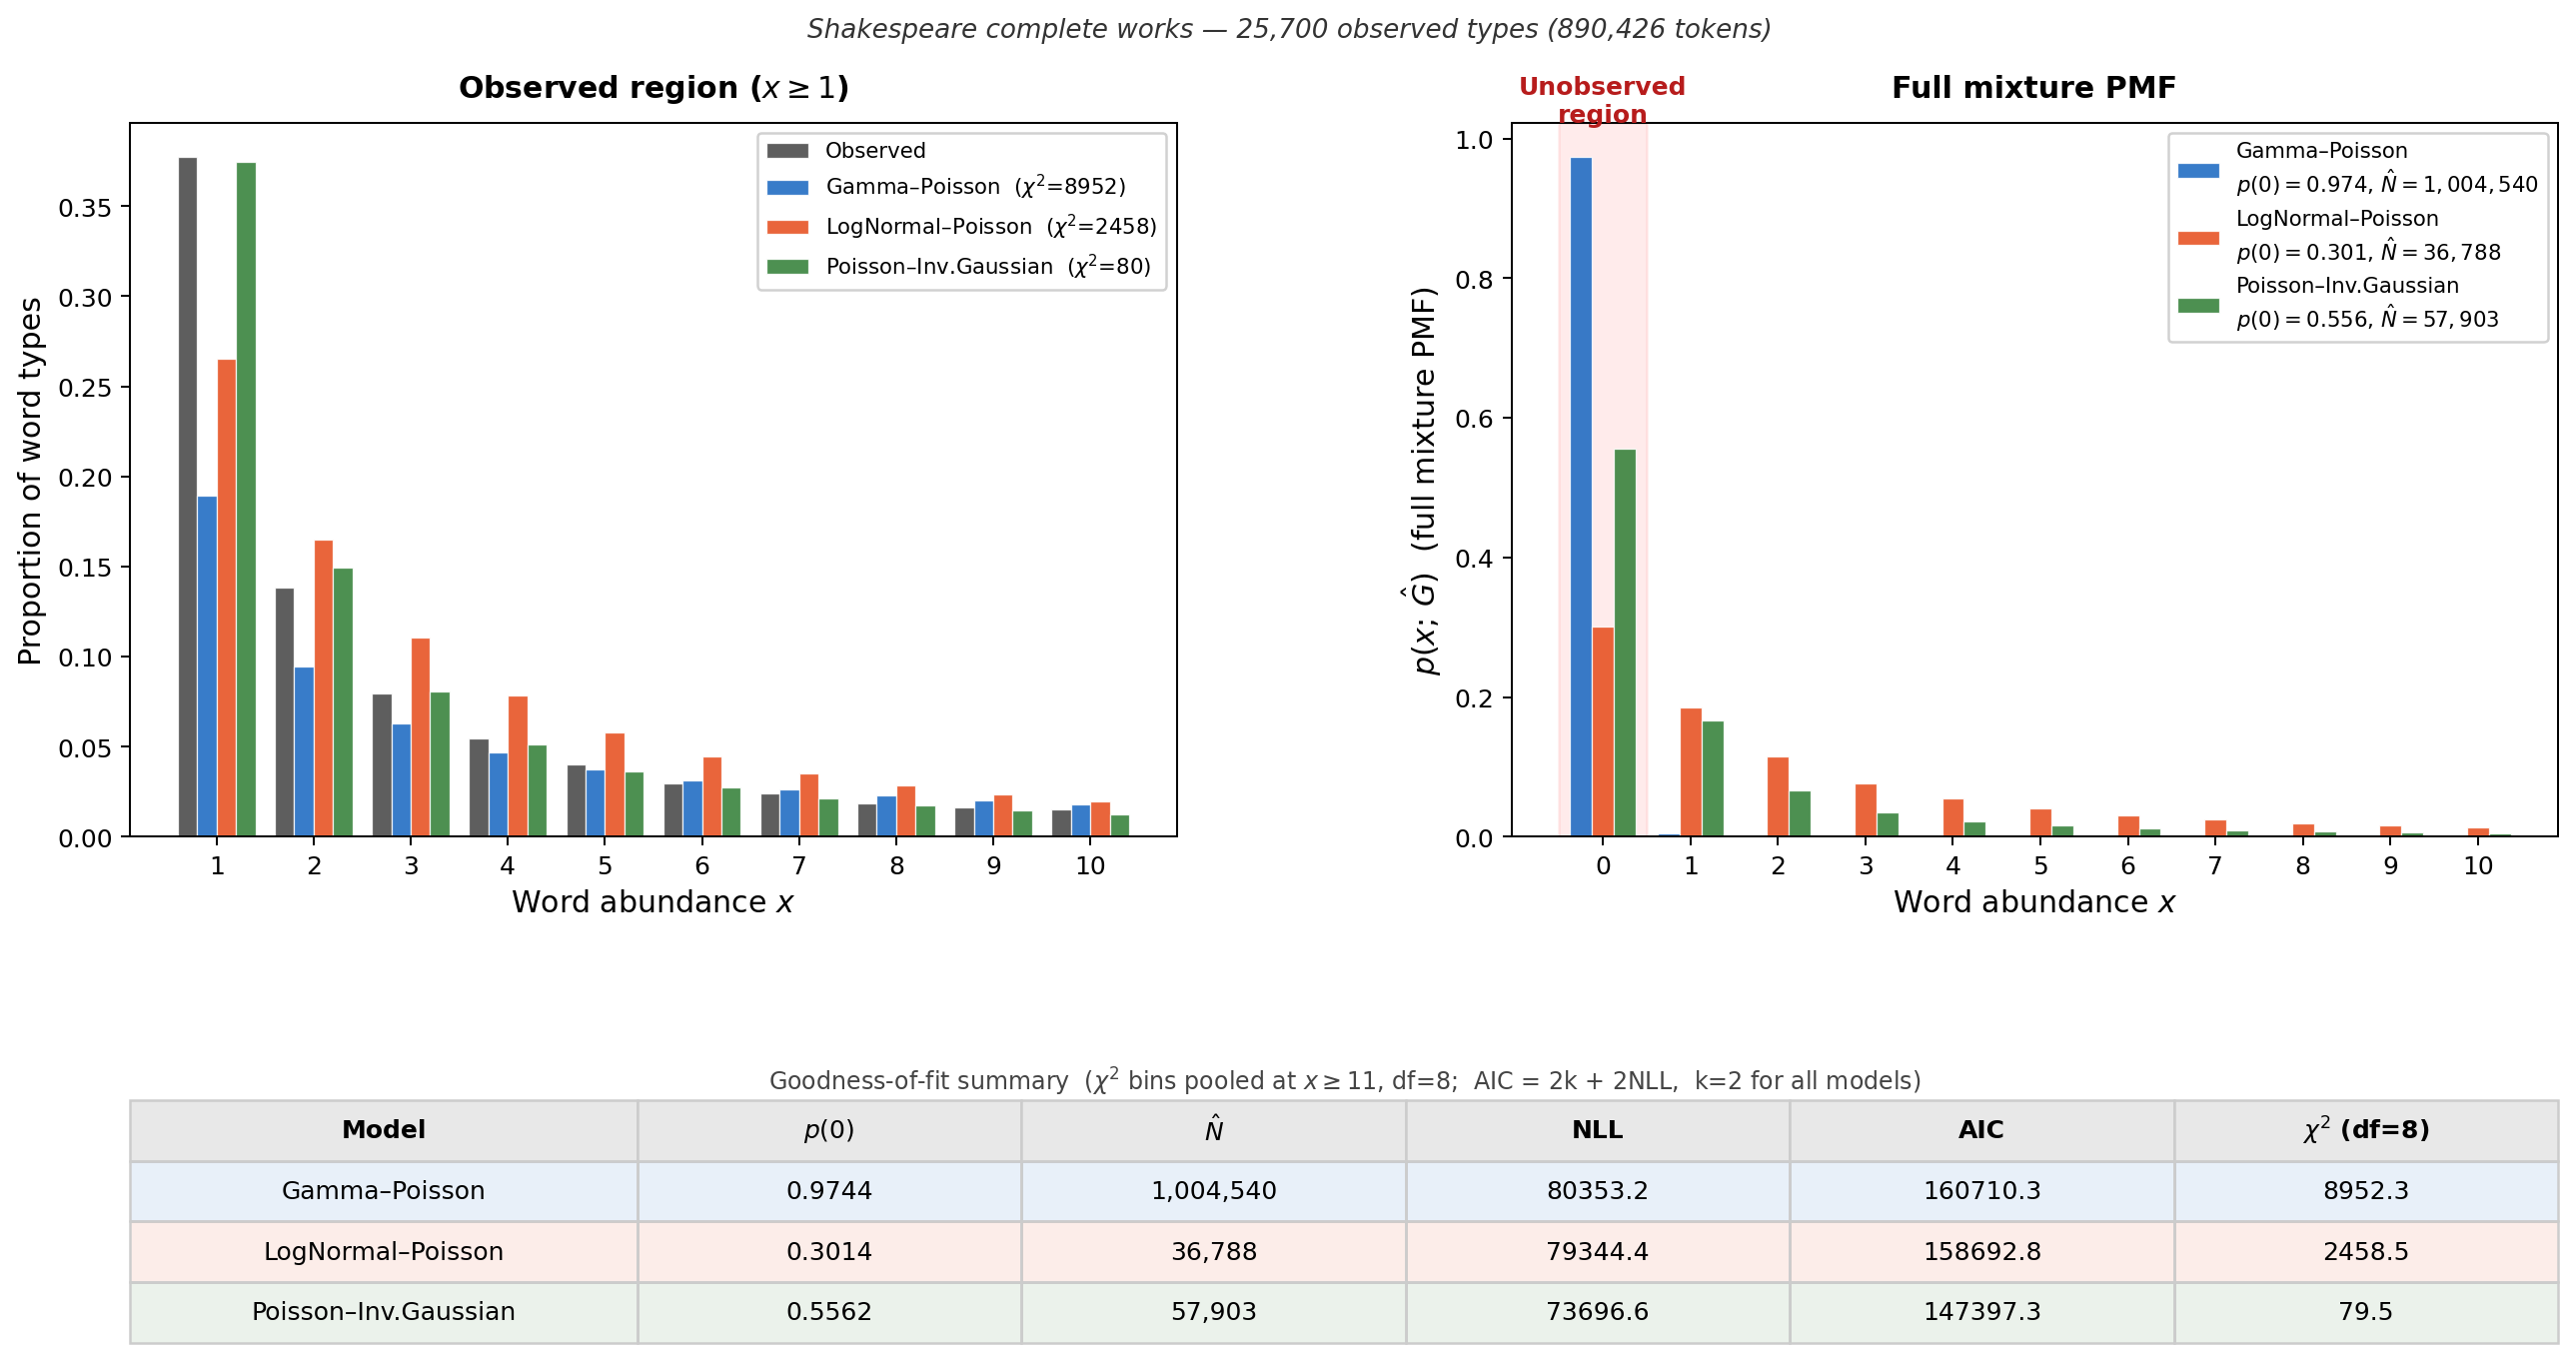
\includegraphics[width=\textwidth]{../code/intuition/mixture_shakespeare.png}
    \caption{Comparison of three parametric Poisson mixture models fitted to the Shakespeare corpus (25,700 observed types, 890,426 tokens). Left: fitted versus observed proportions for $x \geq 1$. Right: full mixture PMF including the extrapolated probability at $x = 0$ (highlighted). The goodness-of-fit summary is shown below the plots.}
    \label{fig:mixture_models}
\end{figure}

To estimate the total number of species under this nonparametric framework, we need a likelihood function that relates the observed frequency counts to the unknowns $N$ and $G$. We derive this by treating the abundances of all $N$ species (observed and unobserved) as independant draws from the mixture distribtion $p(x;G)$.

\paragraph{The likelihood.}
Under the mixture model, the $N$ species abundances are independent draws from a distribution with probability mass function $p(x; G)$. Since $n_0 = N - S_{\mathrm{obs}}$ species are unobserved, the full likelihood function for $N$ and $G$ based on all species (observed and undetected) is~\cite{CheeWang2016}
\begin{equation}\label{eq:full_likelihood}
    L(N, G) = \frac{N!}{(N - S_{\mathrm{obs}})! \,\displaystyle\prod_{x 
    \geq 1} f_x!} \; \bigl\{p(0; G)\bigr\}^{N - S_{\mathrm{obs}}} 
    \prod_{x \geq 1} \bigl\{p(x; G)\bigr\}^{f_x}\,.
\end{equation}
The first factor $\{p(0;G)\}^{N - S_{\mathrm{obs}}}$ accounts for the $N - S_{\mathrm{obs}}$ species that were never observed, each independently having probability $p(0;G)$ of being missed. The second factor accounts for the observed frequency counts. Both $N$ and $G$ are unknown and must be estimated jointly.
 
Sanathanan~\cite{sanathanan1972} showed that the full likelihood decomposes as $L(N, G) = L_m(N, G) \times L_c(G)$, where $L_m$ is a binomial likelihood for $S_{\mathrm{obs}}$ given $N$ and $p(0;G)$, and $L_c$ is the conditional likelihood of the observed frequency counts given $S_{\mathrm{obs}}$, based on the zero-truncated mixture distribution. This decomposition gives rise to two estimation approaches:
\begin{itemize}
    \item The \textbf{conditional approach} first estimates $G$ by maximizing $L_c(G)$ (fitting the zero-truncated data), then estimates $N$ from $L_m$ via
    \begin{equation}\label{eq:horvitz_thompson}
        \hat{N} = \left\lfloor \frac{S_{\mathrm{obs}}}{1 - p(0; 
        \hat{G})} \right\rfloor\,.
    \end{equation}
    \item The \textbf{unconditional approach} jointly maximizes $L(N,G)$ over both $N$ and $G$. Wang and Lindsay~\cite{wanglindsay2005} showed that the resulting estimate also satisfies  Equation~\eqref{eq:horvitz_thompson}.
\end{itemize}
In both cases, the estimation of $N$ reduces to estimating $p(0;G)$ well. This makes the choice of mixture model critical, particularly its behavior near $\lambda = 0$.

\paragraph{Likelihood decomposition.}
Each of the $N$ species is independently either observed (with probability $1 - p(0;G)$) or missed (with probability $p(0;G)$). The number of observed species therefore follows a binomial distribution:
\[
S_{\mathrm{obs}} \sim \mathrm{Binomial}\bigl(N,\; 1 - p(0;G)\bigr)\,.
\]
This lets us factor the full likelihood~\eqref{eq:full_likelihood} as $L(N,G) = L_m(N,G) \times L_c(G)$~\cite{sanathanan1972}, where
\begin{equation}\label{eq:marginal_likelihood}
    L_m(N,G) = \binom{N}{S_{\mathrm{obs}}} 
    \bigl[1 - p(0;G)\bigr]^{S_{\mathrm{obs}}} 
    \bigl[p(0;G)\bigr]^{N - S_{\mathrm{obs}}}
\end{equation}
is the marginal likelihood of observing exactly $S_{\mathrm{obs}}$ species, and
\begin{equation}\label{eq:conditional_likelihood}
    L_c(G) = \frac{S_{\mathrm{obs}}!}{\displaystyle\prod_{x \geq 1} f_x!} 
    \prod_{x \geq 1} \left[\frac{p(x;\, G)}{1 - p(0;\, G)}\right]^{f_x}
\end{equation}
is the conditional likelihood of the observed frequency counts given $S_{\mathrm{obs}}$. The cell probabilities in $L_c$ are precisely those of the zero-truncated mixture distribution:
\begin{equation}\label{eq:zero_truncated}
    p^+(x;\, G) = \frac{p(x;\, G)}{1 - p(0;\, G)}\,, \qquad x \geq 1\,,
\end{equation}
so that, conditional on $S_{\mathrm{obs}}$, the observed abundances behave as $S_{\mathrm{obs}}$ independent draws from $p^+(\cdot\,; G)$. One can verify the decomposition by multiplying~\eqref{eq:marginal_likelihood} and~\eqref{eq:conditional_likelihood} and recovering~\eqref{eq:full_likelihood}.

\paragraph{The conditional approach and the estimator $\hat{N}$.}
The conditional approach proceeds in two stages. First, estimate the mixing distribution by maximizing $L_c(G)$ over $G$, yielding $\hat{G}_c$. Since $L_c$ depends only on the zero-truncated probabilities, this step uses only the observed frequency counts and does not involve $N$. Second, with $\hat{G}_c$ fixed, estimate $N$ from the marginal likelihood $L_m(N, \hat{G}_c)$. Writing $q = 1 - p(0;\hat{G}_c)$ for the estimated detection probability, $L_m$ becomes a binomial likelihood in the single unknown $N$:
\[
L_m(N) = \binom{N}{S_{\mathrm{obs}}} q^{S_{\mathrm{obs}}} (1-q)^{N - S_{\mathrm{obs}}}\,.
\]
To find the integer maximizer, consider the likelihood ratio of consecutive values:
\[
\frac{L_m(N+1)}{L_m(N)} 
= \frac{\binom{N+1}{S_{\mathrm{obs}}}}{\binom{N}{S_{\mathrm{obs}}}} 
  \cdot (1-q)
= \frac{N+1}{N+1-S_{\mathrm{obs}}} \cdot (1-q)\,.
\]
This ratio exceeds $1$ (i.e., the likelihood is still increasing) if and only if
\[
(N+1)(1-q) > N + 1 - S_{\mathrm{obs}} 
\quad\Longleftrightarrow\quad 
N < \frac{S_{\mathrm{obs}}}{q} - 1\,.
\]
Therefore the likelihood increases for all $N < S_{\mathrm{obs}}/q - 1$ and decreases once $N \geq S_{\mathrm{obs}}/q - 1$, giving the integer-valued maximum likelihood estimator
\begin{equation}\label{eq:N_hat_derived}
    \hat{N} = \left\lfloor \frac{S_{\mathrm{obs}}}{q} \right\rfloor 
    = \left\lfloor \frac{S_{\mathrm{obs}}}{1 - p(0;\,\hat{G}_c)} \right\rfloor\,.
\end{equation}
The floor function arises because $N$ must be an integer: when $S_{\mathrm{obs}}/q$ is not an integer, the likelihood peaks between $\lfloor S_{\mathrm{obs}}/q \rfloor$ and $\lceil S_{\mathrm{obs}}/q \rceil$, and the ratio test shows the likelihood is maximized at the largest integer below $S_{\mathrm{obs}}/q$.

This estimator has a natural interpretation as a Horvitz--Thompson-type correction: we observe $S_{\mathrm{obs}}$ species, each detected with probability $q$, so the total population is approximately $S_{\mathrm{obs}} / q$. The quality of $\hat{N}$ depends entirely on how well $p(0;\hat{G}_c)$ is estimated, which in turn depends on the choice of mixture model and its behavior near $\lambda = 0$.

\paragraph{The boundary problem.}
The difficulty is that $p(0;G) = \int_0^\infty e^{-\lambda}\,dG(\lambda)$ is sensitive to the mass $G$ places near $\lambda = 0$: species with very small rates contribute the most to $p(0;G)$, yet they are precisely the species least likely to appear in the observed data. Since the zero-truncated frequencies barely constrain $G$ in this region, small differences in the estimated shape of $G$ near zero can shift $p(0;\hat{G})$ substantially, and because $\hat{N} = S_{\mathrm{obs}}/(1 - p(0;\hat{G}))$, even a modest increase in $p(0;\hat{G})$ toward $1$ causes $\hat{N}$ to explode.
(GRAPH EXAMPLE)

\subsection{Frequency-ratio regression (Breakaway)}\label{sec:breakaway}

The Breakaway method, developed by Willis and Bunge~\cite{willisbunge2015}, takes a different approach to estimating species richness: instead of fitting a distributional model to the abundances, it works directly with the ratios of consecutive frequency counts. Crucially, it does not assume a mixed Poisson model, departing from the framework of Section~\ref{sec:mixture_models}.

The classical estimators presented in Section~\ref{sec:estimators} rely on only $f_1$ and $f_2$ (or up to $f_4$ for iChao1), and can perform poorly on datasets characterized by a large number of rarely observed species, a high singleton count, and a long tail of very abundant species, precisely the pattern exhibited by word frequency data. Breakaway addresses this by using many frequency ratios $f_2/f_1, \ldots f_{j+1}/f_{j}, \ldots$ to fit a smooth curve, then extrapolating back to $j = 0$ to estimate $f_0$. This borrows strength from the entire tail of the distribution rather than relying on the first few counts alone.

\paragraph{How the method works.}
Let $f_1, f_2, \ldots, f_n$ be the observed frequency counts. Since the total number of species satisfies $S = f_0 + \sum_{j=1}^{n} f_j = f_0 + S_{\mathrm{obs}}$, the problem reduces to estimating $f_0$. Breakaway fits a rational function fo the form
\begin{equation}\label{eq:breakaway_ratio}
    \frac{f_{j+1}}{f_j} = \frac{\beta_0 + \beta_1 \, j}{1 + \beta_2 
    \, j + \beta_3 \, j^2}
\end{equation}
to the observed ratios using heteroscedastic nonlinear regression.\footnote{That is, the regression accounts for the fact that the variance of the errors is not constant across the data points.} Setting $j = 0$ in the fitted model gives the predicted
ratio $f_1 / \hat{f}_0 = \hat{\beta}_0$, so that
\begin{equation}\label{eq:breakaway_f0}
    \hat{f}_0 = \frac{f_1}{\hat{\beta}_0}\,, \qquad
    \hat{S} = S_{\mathrm{obs}} + \hat{f}_0\,.
\end{equation}

In practice, Breakaway does not fit a single model. It considers a family of rational functions of increasing complexity and selects the most simplest one satisfying three conditions: $\hat{\beta}_0 > 0$ (so that $\hat{f}_0$ is positive), no singularities in the domain of the observed ratios, and numerical convergence~\cite{willisbunge2015}. The issue of negative unobserved diversity estimators is as old as the problem itself: Fisher, Corbet, and Williams (1943) recognized it when fitting the negative binomial distribution to Malayan butterfly data. (SHOW THIS EXAMPLE)

\vspace{1em}

Specifically, since $\hat{f}_0 = f_1 / \hat{\beta}_0$, the approximate
variance of $\hat{f}_0$ is
\begin{equation}
    \widehat{\mathrm{Var}}(\hat{f}_0)
    \approx f_1 \hat{\beta}_0^{-2}
    \left(1 - \frac{f_1}{n} + f_1 \hat{\beta}_0^{-2}\,
    \widehat{\mathrm{Var}}(\hat{\beta}_0)\right),
\end{equation}

where $\widehat{\mathrm{Var}}(\hat{\beta}_0)$ is the estimated variance of $\hat{\beta}_0$ from the nonlinear regression, and the variance of the total estimate is ~\cite{willisbunge2015}

    \begin{equation}
        \widehat{\mathrm{Var}}
        (\hat{S}) \approx
        n\hat{f}_0 / (n + \hat{f}_0) +
        \widehat{\mathrm{Var}}(\hat{f}_0)
    \end{equation}

\vspace{1em}

Figure~\ref{fig:breakaway_ratio_example} illustrates the extrapolation step in the Breakaway method. The observed points are the consecutive frequency ratios \(f_{j+1}/f_j\), computed from the abundance frequency counts. We can see the fitted smooth rational function and the fitted value at \(j=0\) estimates \(\hat{\beta}_0 = f_1/\hat f_0\), so the number of unseen types is obtained as \(\hat f_0 = f_1/\hat{\beta}_0\). The different curves show how the fit changes when more ratio terms are included.


\begin{figure}[ht]
    \centering
    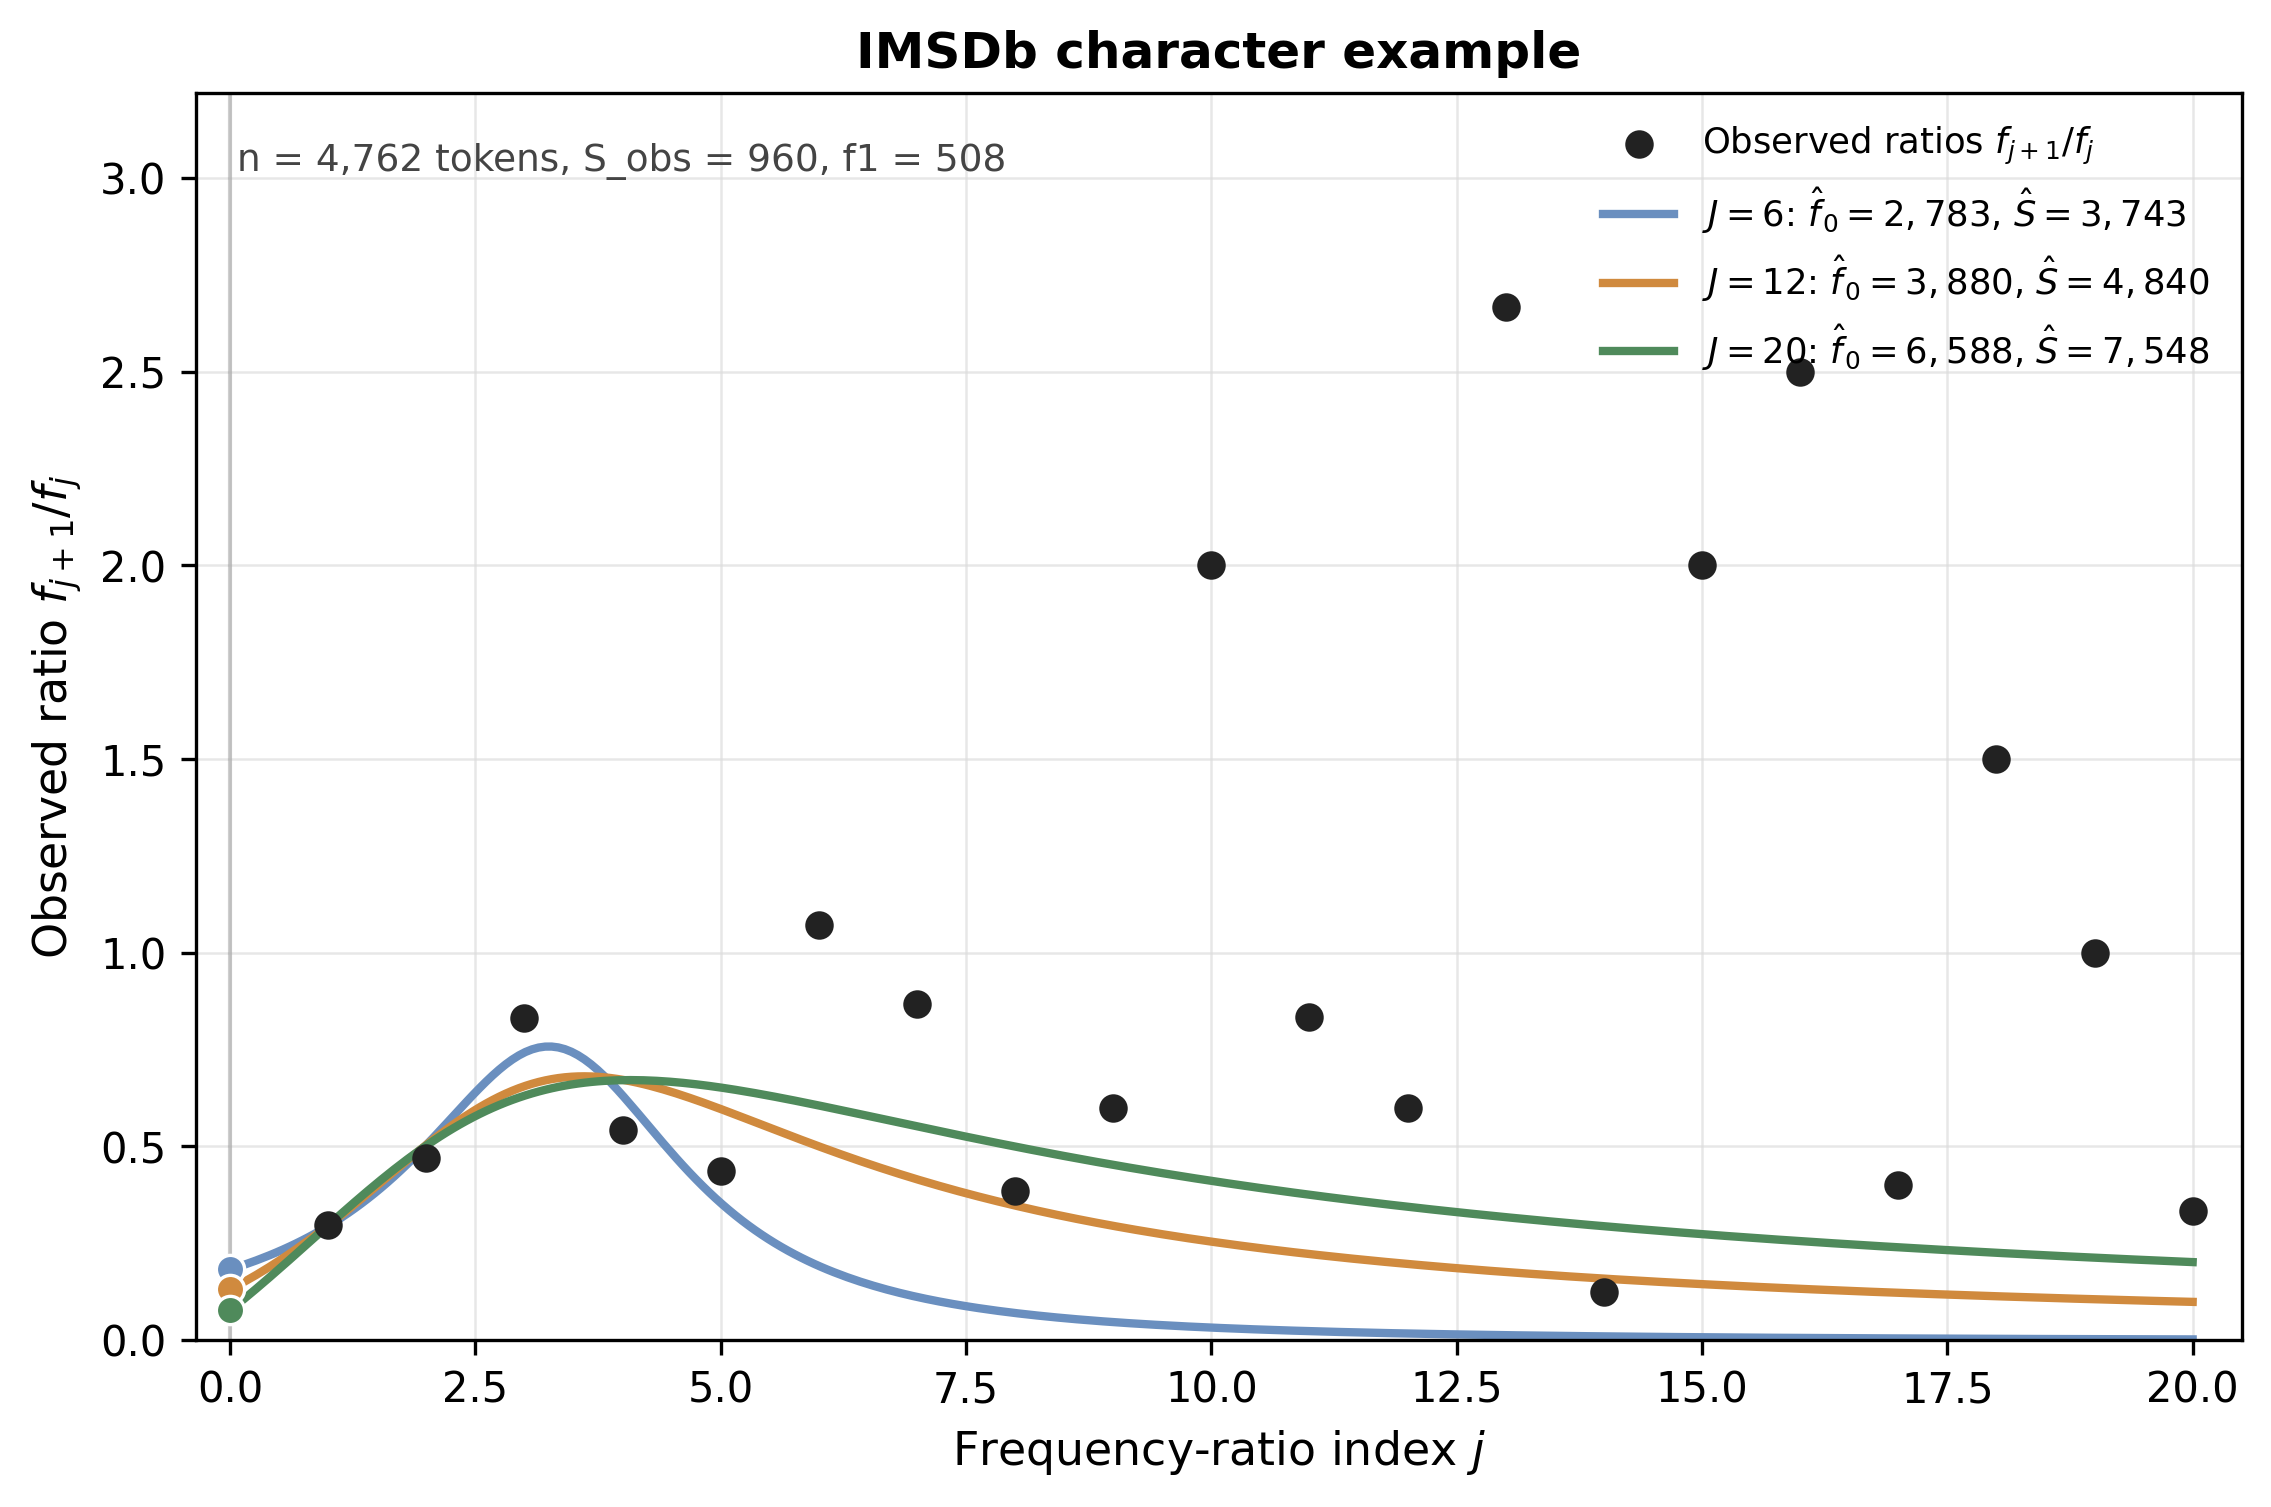
\includegraphics[width=\textwidth]{../code/intuition/breakaway_ratio_example.png}
    \caption{Breakaway frequency-ratio regression for one example corpus item. Black points show the observed ratios \(f_{j+1}/f_j\). The colored curves are rational-function fits using ratios up to different maximum indices \(J\). Their extrapolated values at \(j=0\) determine \(\hat{\beta}_0\), and hence the estimate \(\hat f_0 = f_1/\hat{\beta}_0\).}
    \label{fig:breakaway_ratio_example}
\end{figure}

\paragraph{Limitations.}
As we have seen previously we have have no guarantee that the estimate is positive. If $\hat{\beta_0}$ is close to 0 or negative, The estimate $\hat{f_0} = f_1/\hat{\beta_0}$ will have a negative or very high estimate.\\
This method also requires enough data points otherwise we will not have the desired frequency counts. As stated in the Willis paper ~\cite{willisbunge2015}, if the maximum number of observed frequency is 6 or less, then there aren't enough ratios to fit the nonlinear model, and Breakaway can't run.


\subsection{Shape-constrained estimation}
 
\subsubsection{k-monotone distributions: definition and mixture representation}
The nonparametric Poisson mixture model, as we have seen, reduces species richness estimation to the problem of estimating $p(0;G)$. However, it suffers from the boundary problem: the NPMLE (nonparametric Maximum Likelihood Estimator) of $G$ tends to place mass near $\lambda = 0$, which inflates $p(0;G)$ and sends $\hat{N}$ to very high values. This motivates moving to an alternative nonparametric mixture model that retains the flexibility of leaving the mixing distribution unspecified but does not suffer from this instability.

The following strategy follows those ideas: instead of constraining the mixing distribution $G$, we impose a shape constraint directly on the abundance PMF $p$. We require that $p$ belongs to the family of $k$-monotone distributions:

\vspace{1em}

The definition of $k$-monotone distributions is given as follows:
Let $k$ be a positive integer. The \emph{forward difference operator} $\Delta$ acts on a sequence $p \colon \mathbb{N}_0 \to \mathbb{R}$ by
\[
\Delta p(x) = p(x+1) - p(x),
\]
and higher-order differences are defined recursively: the $a$th order forward difference is
\[
\Delta^a p(x) = \sum_{i=0}^{a} \binom{a}{i} (-1)^{i}\, p(x + a - i), \qquad a = 1, 2, \ldots
\]
A discrete distribution with probability mass function $p$ on $\mathbb{N}_0 = \{0, 1, 2, \ldots\}$ is said to be \emph{$k$-monotone} if
\[
(-1)^a \,\Delta^a p(x) \;\geq\; 0 \qquad \text{for all } a = 1, \ldots, k \text{ and all } x \in \mathbb{N}_0.
\]
If the condition holds for all $a \in \mathbb{N}$ (i.e.\ $k = \infty$), the distribution is called \emph{completely monotone}.

\vspace{1em}

For $k = 1$, the condition reduces to $-\Delta p(x) = p(x) - p(x+1) \geq 0$ for all $x$, i.e.\ $p$ is non-increasing. For $k = 2$, it additionally requires $\Delta^2 p(x) = p(x+2) - 2p(x+1) + p(x) \geq 0$, meaning that $p$ is non-increasing \emph{and} convex: the successive decrements $p(x) - p(x+1)$ are themselves non-increasing. Both conditions are natural for species abundance distributions, which are typically right-skewed with their mode at $x = 1$ and a long decreasing tail.

\vspace{1em}

The key structural property of $k$-monotone distributions is that they admit a mixture representation. Lefèvre and Loisel \cite{LefevreLoisel2013} showed that a PMF $p$ on $\mathbb{N}_0$ is $k$-monotone if and only if there exists a sequence of mixing probabilities $(\pi^k_l)_{l \in \mathbb{N}_0}$ with $\pi^k_l \geq 0$ and $\sum_{l \geq 0} \pi^k_l = 1$ such that
\[
p(j) = \sum_{l \geq 0} \pi^k_l \, Q^k_l(j),
\]
where
\[
Q^k_l(j) = \frac{\binom{l - j + k - 1}{k-1}}{\binom{l+k}{l}} \, \mathbf{1}_{\{0 \leq j \leq l\}}
\]
is the \emph{$k$-monotone spline} with support $\{0, 1, \ldots, l\}$. Each spline $Q^k_l$ is itself a discrete distribution concentrated on $l+1$ points, and the mixing weights $\pi^k_l$ describe how the overall abundance distribution is assembled from these components. The weights can be recovered from $p$ via the inversion formula
\[
\pi^k_l = (-1)^k \, \Delta^k p(l) \, \binom{l+k}{l}.
\]

This mixture representation is the analogue of the Poisson mixture from Section~4.1, but with the $k$-monotone splines $Q^k_l$ replacing the Poisson distributions as building blocks. The crucial difference is that the spline $Q^k_0$ (with $l = 0$) is a point mass at the origin: it assigns all its probability to $j = 0$. In the species richness context, a species whose abundance follows $Q^k_0$ would never be observed in any sample. Since something that was never observed cannot contribute to the observed data, we must set $\pi^k_0 = 0$. Applying the inversion formula with $l = 0$ gives $\pi^k_0 = (-1)^k \Delta^k p(0) = 0$, which is equivalent to the constraint
\[
\Delta^k p(0) = p(0) + \sum_{j=1}^{k} (-1)^j \binom{k}{j} p(j) = 0.
\]
This single linear equation links $p(0)$ (the probability that a species goes entirely undetected) to the observed probabilities $p(1), p(2), \ldots, p(k)$. Rearranging in terms of the zero-truncated PMF $p^+(j) = p(j)/(1-p(0))$ yields
\[
\frac{1}{1 - p(0)} = 1 - \sum_{j=1}^{k} (-1)^j \binom{k}{j} p^+(j).
\]
This is precisely what the Poisson mixture framework lacked: a structural constraint that identifies $p(0)$ from the observed data. The boundary problem is resolved not by penalizing mass near $\lambda = 0$, but by working with a model in which $p(0)$ is determined by the shape of the observed distribution. Once $p(0)$ is identified, the estimator $\hat{N} = \lfloor S_{\mathrm{obs}} / (1 - p(0)) \rfloor$ follows directly. This solves the problem of \emph{one cannot see what cannot be seen}.

\vspace{1em}

Figure~\ref{fig:k_monotonicity_examples} gives a visual intuition for the role of the parameter \(k\). We see that large values of \(k\) impose alternating-sign constraints, thus increasing \(k\) restricts the possible shapes of the abundance distribution, making the curve more structured.

\begin{figure}[ht]
    \centering
    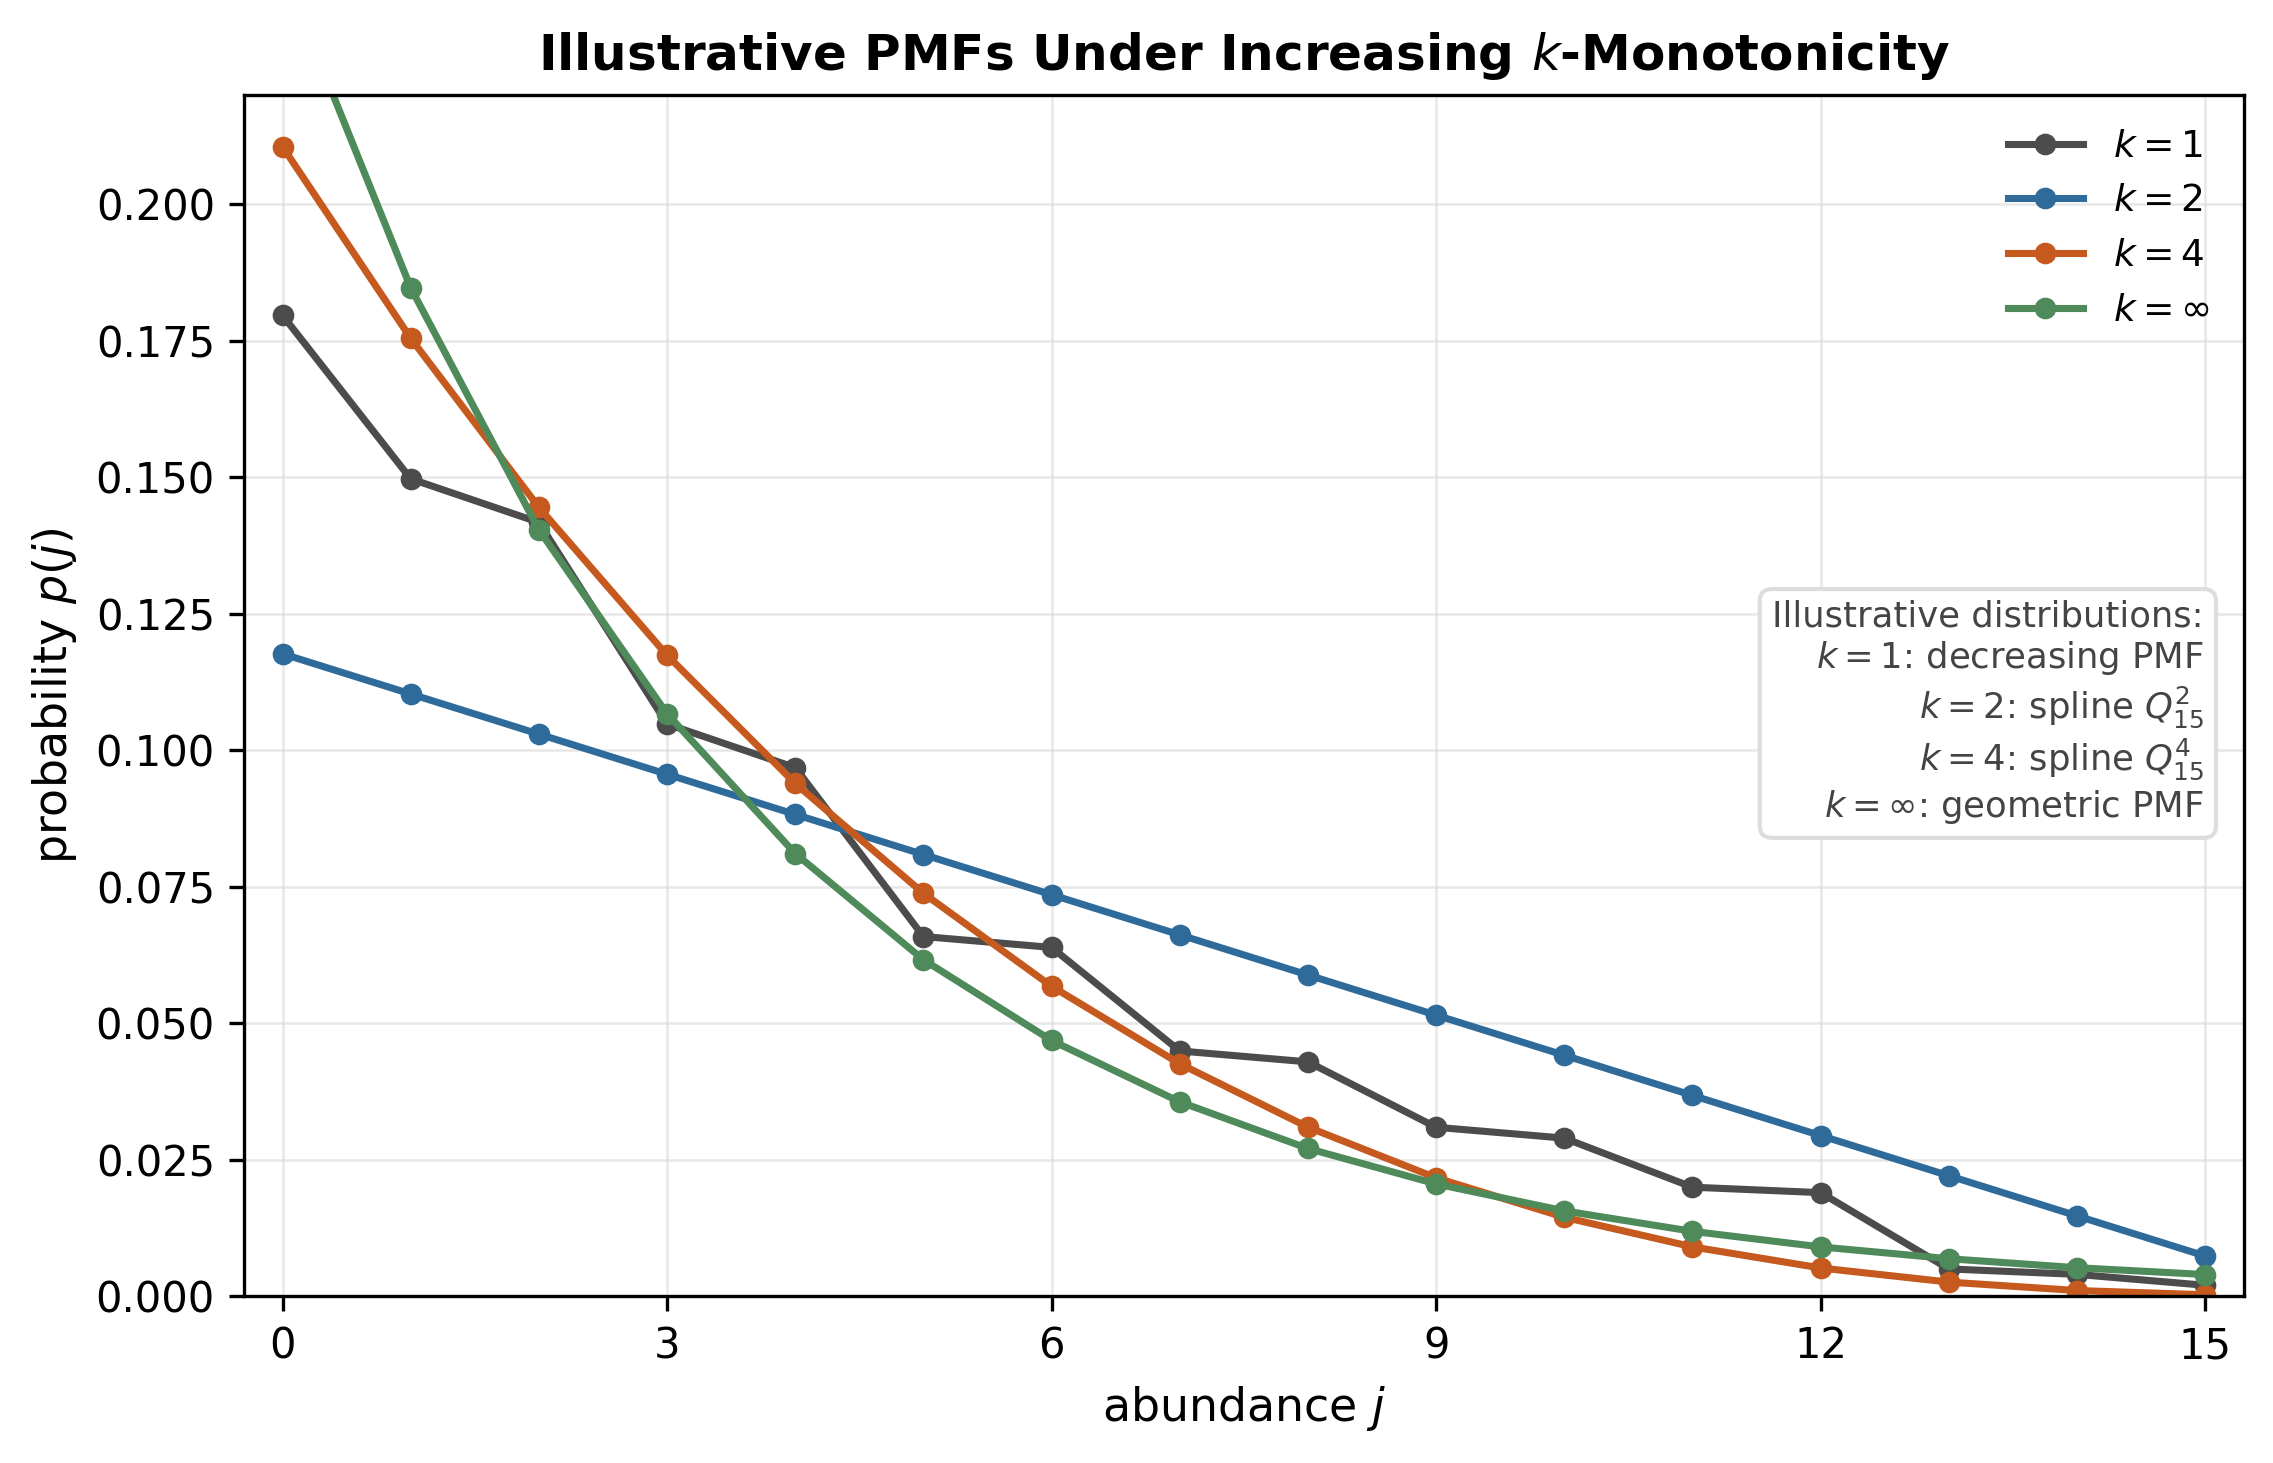
\includegraphics[width=\textwidth]{../code/intuition/k_monotonicity_examples.png}
    \caption{Illustrative probability mass functions satisfying different levels of \(k\)-monotonicity. The \(k=1\) curve is a decreasing PMF, the \(k=2\) and \(k=4\) curves are \(k\)-monotone splines, and the \(k=\infty\) curve is a geometric PMF, which is completely monotone.}
    \label{fig:k_monotonicity_examples}
\end{figure}


\subsubsection{Selection of \texorpdfstring{$k$}{k}}
The value of $k$ controls the shape restriction, a larger k imposes more constraints  and therefore structure and pushes the support points of the NPMLE further from the left boundary. It is important to note that it does not necessarily produce a higher fitted probability at 0. Therefore, the estimate of $\hat{N}$ does not necessarily increase with $k$ \cite{CheeWang2016} .

In practice, the appropriate value of $k$ for a given dataset is unknown, thus its a model selection problem. Since the family of $k$-monotone distributions shrinks as $k$ increases, the maximized log-likelihood $\ell_k(\hat{N}, \hat{G})$ decreases monotonically with $k$. Chee and Wang balance goodness of fit against model complexity by evaluating the Akaike information criterion (AIC) over a grid of $k$ values ranging from $k = 2$ to $k = \infty$, selecting the value that minimizes the AIC.
 
\subsubsection{Complete monotonicity as the limit of \texorpdfstring{$k$}{k}-monotonicity}

As $k$ increases, the family of $k$-monotone distributions becomes increasingly restrictive . A classical result given by Steutel \cite{Steutel1969} characterizes the limiting case: a PMF $p$ on $\mathbb{N}_0$ is completely monotone if and only if it is a mixture of geometric distributions, that is,
\begin{equation}
p(j) = \int_0^1 \alpha(1-\alpha)^j \, dH(\alpha),
\qquad j \in \mathbb{N}_0
\label{eq:cm-mixture}
\end{equation}

where $H$ is a distribution function on $[0,1]$. Thus the geometric distributions play the same role for complete monotonicity as the $k$-monotone splines $Q^k_l$ play for finite $k$, i.e. they are the building blocks from which any completely monotone PMF can be assembled.

Chee and Wang \cite{CheeWang2016} established the connection explicitly by showing that the $k$-monotone mixture PMF converges, as $k \to \infty$, to a mixture of geometric distributions. Balabdaoui and Kulagina \cite{BalabdaouiKulagina2020} formalized this further: if a sequence of $k$-monotone PMFs $(p^k)_{k \in \mathbb{N}}$ has mixing distributions that converge weakly to some distribution $H$ on $[0,1)$, then the sequence converges pointwise to the completely monotone PMF \eqref{eq:cm-mixture}.

\vspace{1em}

With this convergence result we can justify using the completely monotone model whenever the true degree of monotonicity is large. In practice, when the AIC selection of Chee and Wang keeps selecting larger values of $k$, this suggests that the data is approximately completely monotone, and one can work directly with the limiting model. Doing so eliminates the need to select $k$ altogether which is a significant practical advantage, since the differences between $k$- and $(k+1)$-monotonicity become increasingly difficult to detect as $k$ grows.

\subsubsection{The Balabdaoui and Kulagina estimator: \texorpdfstring{$\hat{N}_{\infty}$}{N-infinity}}

Balabdaoui and Kulagina \cite{BalabdaouiKulagina2020} avoid the problem of selecting $k$ by letting it grow logarithmically with the sample size $n$. Define $\bar{\alpha}_n = 1 - \bar{p}_n(1)$, where $\bar{p}_n$ is the empirical estimator of the zero-truncated PMF. The degree of monotonicity is set to
\[
k_n = \left\lfloor \frac{\log n}{2 \log(\bar{\alpha}_n^{1/2} + 1)} 
\right\rfloor,
\]
and the estimator of $N$ is
\[
\hat{N}_{\infty} = \left\lfloor n\left(1 - \sum_{j=1}^{k_n} (-1)^j 
\binom{k_n}{j} \bar{p}_n(j)\right) \right\rfloor.
\]
Under the assumption that $\bar{\alpha}_n \geq (\sqrt{2} - 1)^2$ and that the true PMF is a finite mixture of geometrics, the estimator is asymptotically normal, yielding the confidence interval at level $1 - \alpha$:
\[
\hat{N}_{\infty} \;\pm\; z_{1-\alpha/2}\,\sqrt{n}\,\hat{\sigma}_n, 
\qquad \hat{\sigma}_n^2 = \sum_{l=1}^{k_n} \binom{k_n}{l}^2 
\bar{p}_n(l).
\]

\subsubsection{The bootstrap test for complete monotonicity}
TODO

\section{Data and Methodology}\label{sec:data}

\subsection{What is a word?}

Before implementing our models, we must first specify what we mean by a \emph{word}. This is not entirely straightforward, since words can be counted in different ways depending on the linguistic conventions adopted. The issue becomes particularly important when comparing texts across different languages, as languages differ substantially in how words are formed. For example, German productively forms compound words, allowing the creation of long expressions that may be considered distinct lexical items.

A first distinction is between \emph{tokens} and \emph{types}. A token refers to each individual occurrence of a word in a text, whereas a type refers to a distinct word form. For example, in the sentence
\[
\textit{the cat and the dog},
\]
there are five tokens but only four types, since the word \textit{the} appears twice.

Another important distinction concerns whether different grammatical forms of a word should be treated as separate types. For example, one may either:
\begin{itemize}
    \item treat \emph{run}, \emph{running}, and \emph{ran} as different words, or
    \item group them together under the same base form.
\end{itemize}

The latter approach is known as \emph{lemmatization}. A \emph{lemma} is the canonical or dictionary form of a word, so that conjugated or plural forms are counted together. Under this convention, \emph{run}, \emph{running}, and \emph{ran} are all associated with the lemma \emph{run}.

In this work, we consider both approaches the approach of counting tokens. This method was used for estimating the well known example about vocabulary richness of \emph{Shakespeare}. And because of convenience and sake of comparison, we will make use of the same.

\subsection{Data sources}

Our analysis draws on four data sources: one established reference corpus and three sources of spoken or dialogue-based English.

\paragraph{Shakespeare corpus.}  As a baseline for replication and comparison, we use the word frequency counts from Spevack's concordance  \cite{Spevack1968}, comprising 890,426 tokens and 25,700 observed types  across the complete works of Shakespeare. This dataset has been widely used  in the species richness literature  \cite{BalabdaouiKulagina2020, CheeWang2016} and allows us to verify our  implementations against published results.

\paragraph{Internet Movie Script Database (IMSDb).} 
We downloaded scripts from approximately 1,200 English-language films from the Internet Movie Script Database. We applied preprocessing tools to extract only the dialogue portions, discarding stage directions and scene descriptions. Each character's lines were then aggregated across the entire film. To ensure a minimum sample size, we retained only characters with at least 500 tokens, corresponding to roughly 3--5 minutes of speech at a comfortable speaking pace of 100--150 words per minute.

\paragraph{British National Corpus (BNC).} 
We used the spoken component of the British National Corpus, which contains transcriptions of spontaneous British English conversation and other spoken registers.

\paragraph{Santa Barbara Corpus of Spoken American English.} 
This corpus consists of transcriptions of naturally occurring spoken interactions in American English.

\vspace{1em}

Our analysis combines one reference literary corpus with three corpora of spoken or dialogue-based English.\footnote{See Appendix~\ref{app:sources} for URLs and access information for all data sources.}


\subsection{Preprocessing}

All texts were lowercased and stripped of punctuation. We removed all the number and filler words, the contractions where left as a single type.

For each speaker or character, we computed the abundance frequency counts $f_1, f_2, \ldots$ as defined in Section~\ref{sec:framework}: $f_k$ is the number of types appearing exactly $k$ times in that speaker's text. These frequency counts serve as the input to all the estimators described in Sections~\ref{sec:estimators} and~\ref{sec:shape}.


\section{Results}\label{sec:results}

\subsection{Shakespeare replication baseline}

We first use the full Shakespeare corpus as a replication baseline for the estimators. This corpus is not used in the cross-language spoken-language comparison, since it is a written literary corpus rather than spoken language.

\begin{table}[htbp]
    \centering
    \resizebox{\textwidth}{!}{
    \begin{tabular}{lrrrrrrrrrr}
        $x$ & 1 & 2 & 3 & 4 & 5 & 6 & 7 & 8 & 9 & 10 \\
        \hline
        0+ & 9704 & 3562 & 2050 & 1408 & 1028 & 759 & 620 & 475 & 415 & 393 \\
        10+ & 292 & 264 & 217 & 231 & 192 & 176 & 165 & 143 & 144 & 146 \\
        20+ & 124 & 103 & 89 & 97 & 87 & 89 & 76 & 84 & 59 & 82 \\
        30+ & 74 & 49 & 60 & 56 & 57 & 51 & 34 & 36 & 42 & 40 \\
        40+ & 43 & 52 & 33 & 34 & 23 & 36 & 33 & 33 & 35 & 34 \\
        50+ & 24 & 17 & 20 & 34 & 27 & 22 & 13 & 21 & 20 & 18 \\
        60+ & 25 & 17 & 18 & 23 & 23 & 13 & 13 & 10 & 16 & 13 \\
        70+ & 16 & 8 & 14 & 17 & 9 & 17 & 8 & 14 & 17 & 11 \\
        80+ & 14 & 16 & 10 & 15 & 8 & 14 & 9 & 6 & 11 & 10 \\
        90+ & 3 & 9 & 8 & 12 & 8 & 5 & 8 & 10 & 6 & 5 \\
    \end{tabular}}
    \caption{Frequency spectrum of the processed full Shakespeare corpus. Each entry is the number of distinct word types occurring exactly $x$ times, where the row label gives the tens digit; for example, the first row gives $f_1,\ldots,f_{10}$ and the second row gives $f_{11},\ldots,f_{20}$. The full corpus has 890,426 tokens and 25,700 observed word types.}
    \label{tab:results_shakespeare_frequency_table}
\end{table}

\paragraph{Table interpretation placeholder.}
TODO: Compare this frequency spectrum with the published Shakespeare table. If the published table has different singleton and doubleton counts, explain whether this comes from a different source, tokenization, lemmatization, or preprocessing convention.

\begin{table}[htbp]
    \centering
    \resizebox{\textwidth}{!}{
    \begin{tabular}{lrrrrrrr}
        Estimator & Tokens $n$ & $S_{\mathrm{obs}}$ & $f_1$ & $f_2$ & Coverage & $\hat{S}$ & $\hat{S}/S_{\mathrm{obs}}$ \\
        \hline
        Chao1 & 890426 & 25700 & 9704 & 3562 & 0.9891 & 38918.3 & 1.5143 \\
        iChao1 & 890426 & 25700 & 9704 & 3562 & 0.9891 & 41506.7 & 1.6150 \\
        ACE & 890426 & 25700 & 9704 & 3562 & 0.9891 & 70942.2 & 2.7604 \\
        Jackknife1 & 890426 & 25700 & 9704 & 3562 & 0.9891 & 35404.0 & 1.3776 \\
        Jackknife2 & 890426 & 25700 & 9704 & 3562 & 0.9891 & 41546.0 & 1.6166 \\
        Breakaway & 890426 & 25700 & 9704 & 3562 & 0.9891 & -- & -- \\
    \end{tabular}}
    \caption{Summary of Shakespeare replication estimates for the processed full Shakespeare corpus. Breakaway is undefined here because the fitted extrapolation parameter is negative.}
    \label{tab:results_shakespeare_estimator_summary}
\end{table}

\paragraph{Table interpretation placeholder.}
TODO: Explain the Shakespeare estimator table, especially the difference between lower-bound estimators and ACE, and mention that Breakaway is not stable for this full-corpus frequency spectrum.

\begin{figure}[htbp]
    \centering
    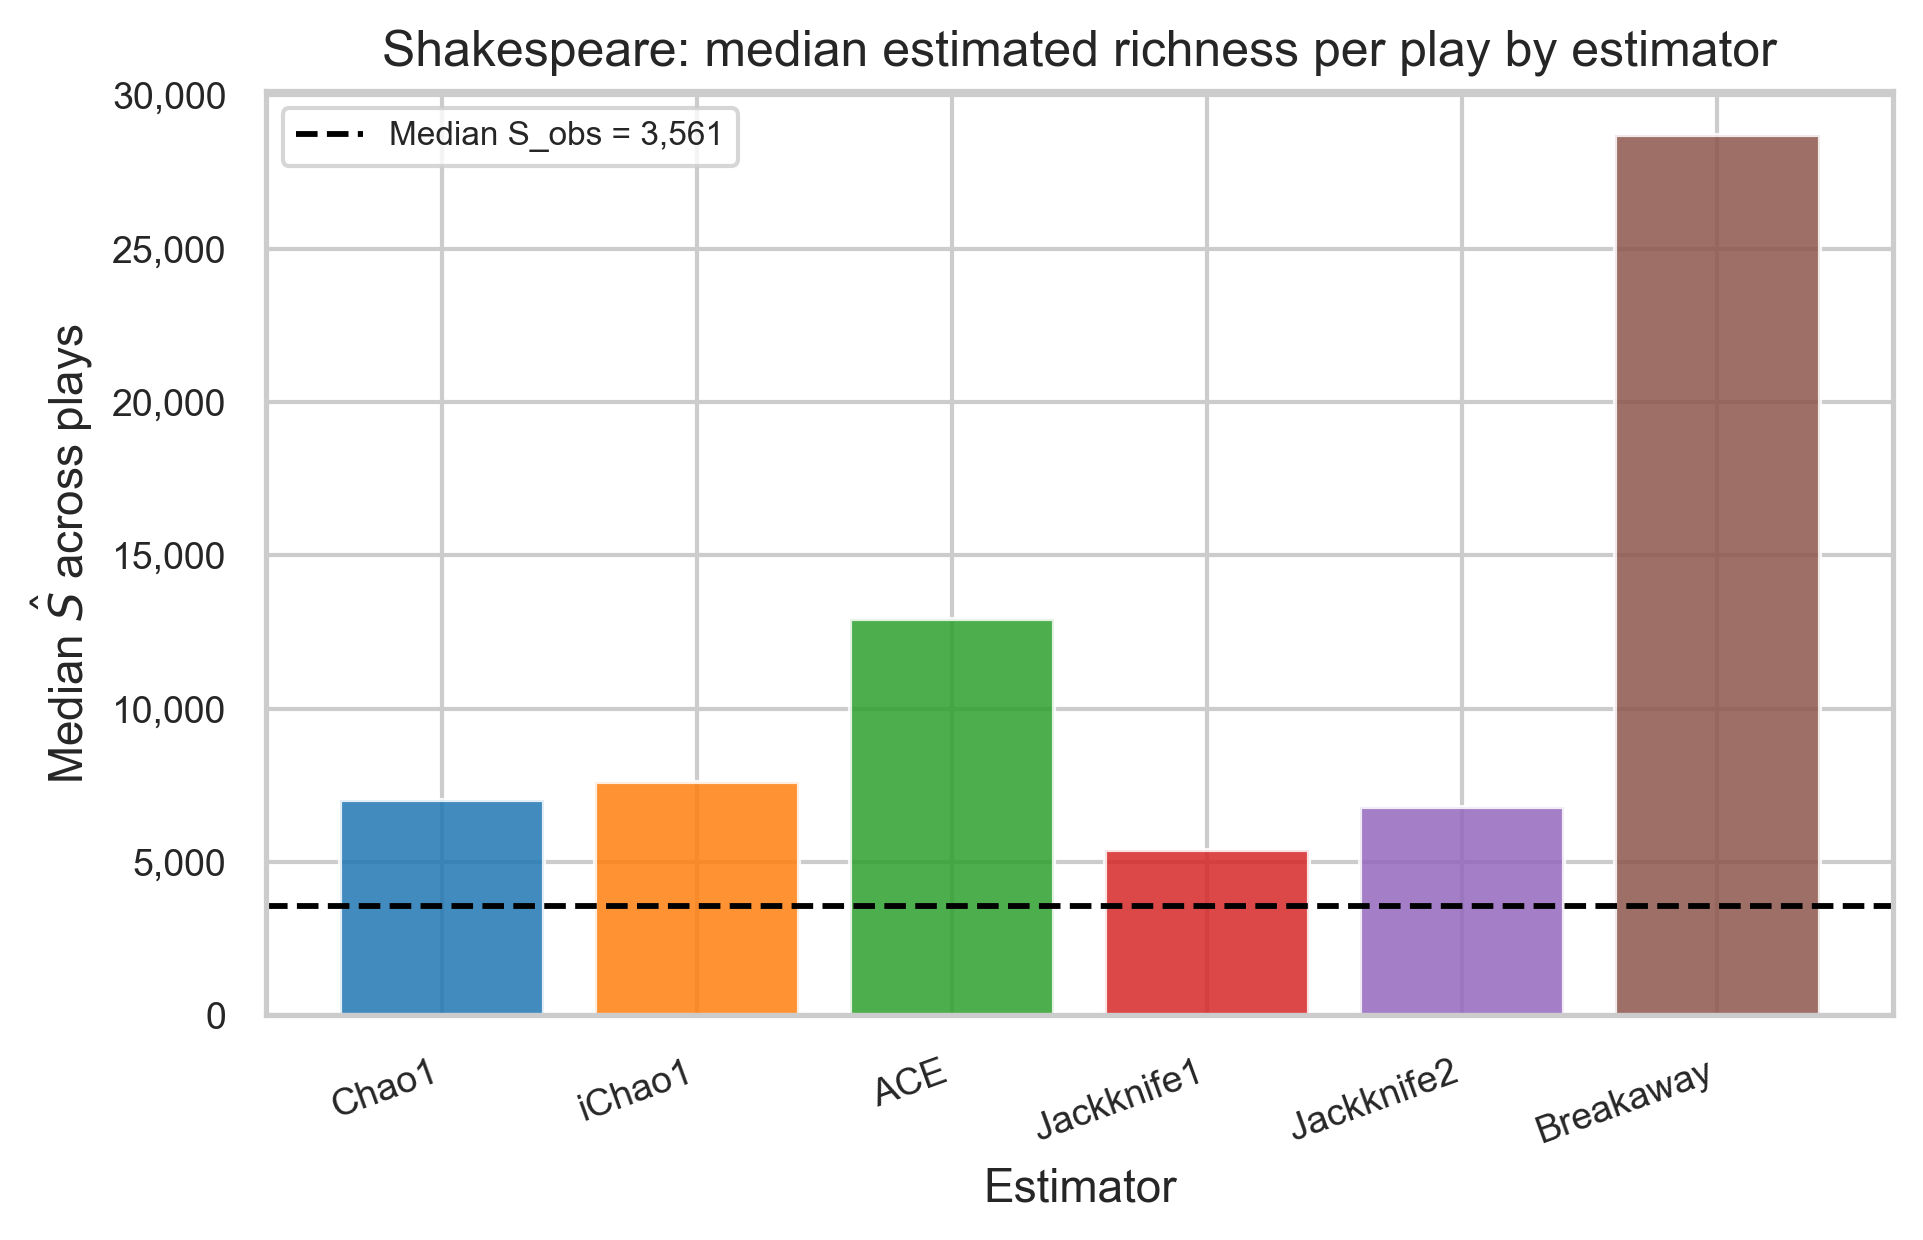
\includegraphics[width=\textwidth]{../results/figures/shakespeare_estimator_comparison.png}
    \caption{Estimated vocabulary richness for the Shakespeare replication baseline, comparing the estimators implemented in the analysis pipeline.}
    \label{fig:results_shakespeare_estimator_comparison}
\end{figure}

\paragraph{Interpretation placeholder.}
TODO: Explain how the estimators compare on Shakespeare, which ones are conservative or aggressive, and whether the results look plausible relative to the published Shakespeare analyses.

\begin{figure}[htbp]
    \centering
    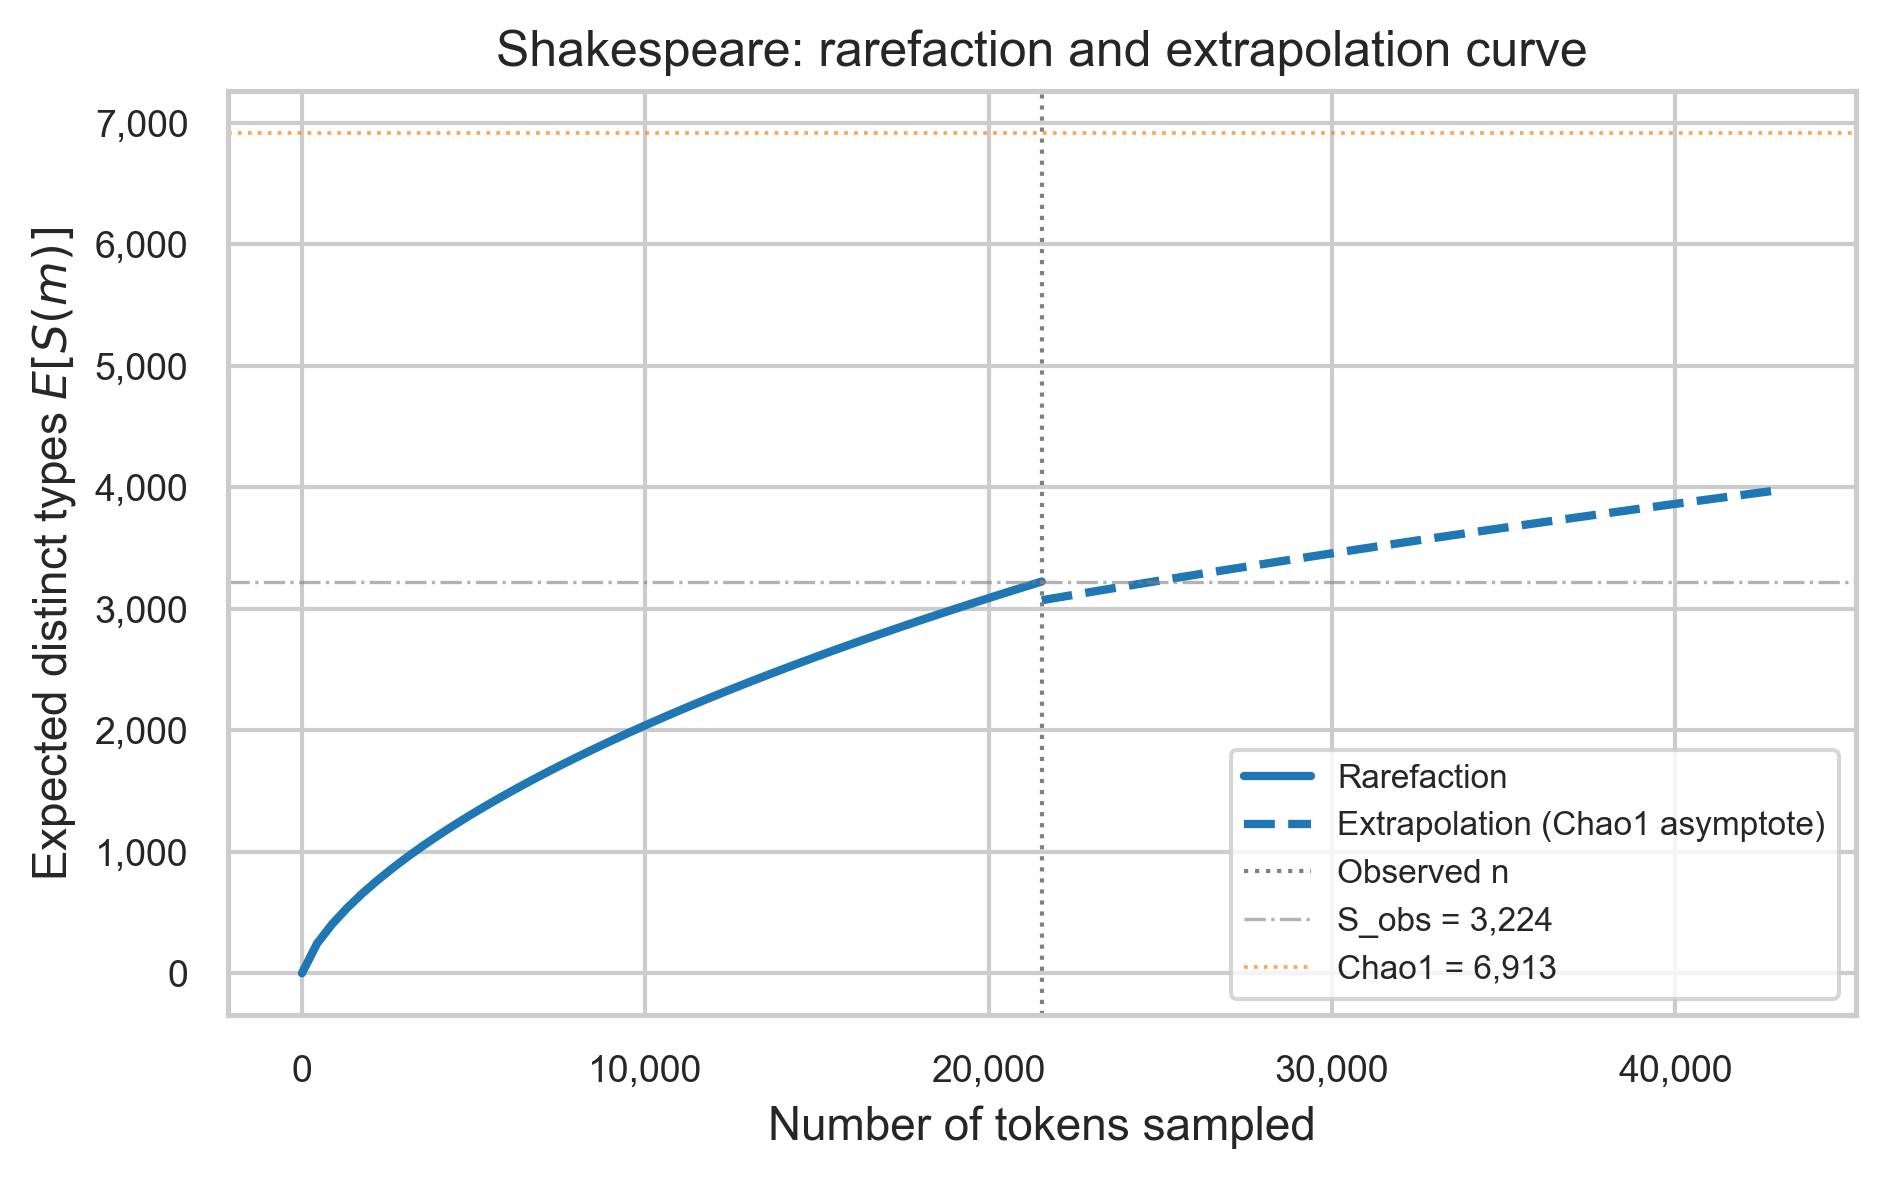
\includegraphics[width=\textwidth]{../results/figures/rarefaction_extrapolation_shakespeare.png}
    \caption{Rarefaction and extrapolation curve for a representative Shakespeare unit.}
    \label{fig:results_rarefaction_extrapolation_shakespeare}
\end{figure}

\paragraph{Interpretation placeholder.}
TODO: Explain whether the Shakespeare curve is still increasing at the observed sample size and what the extrapolation suggests about unseen vocabulary.

\subsection{Corpus and language overview}

We next summarize the spoken and dialogue-based corpora used for the main multilingual analysis. In the cross-language comparison, English consists of IMSDb, BNC, and the Santa Barbara Corpus; French consists of CLAPI; and German consists of DGD.

\begin{table}[htbp]
    \centering
    \resizebox{\textwidth}{!}{
    \begin{tabular}{llrrrr}
        Language & Corpora included & Number of units & Total tokens & Median tokens & Mean coverage \\
        \hline
        English & bnc, imsdb, sbcorpus & 5517 & 6675363 & 815 & 0.7197 \\
        French & clapi & 10813 & 160251286 & 1927 & 0.8104 \\
        German & dgd & 47 & 68141 & 1485 & 0.7782 \\
    \end{tabular}}
    \caption{Language-level overview of the spoken/dialogue corpora used in the cross-language comparison. Shakespeare is excluded from this table.}
    \label{tab:results_language_corpus_overview}
\end{table}

\paragraph{Table interpretation placeholder.}
TODO: Explain the language-level corpus overview, especially the imbalance in number of units and total tokens.

\begin{table}[htbp]
    \centering
    \resizebox{\textwidth}{!}{
    \begin{tabular}{llrrrrrrr}
        Corpus & Language & Units & Total tokens & Median tokens & Min tokens & Max tokens & Median $S_{\mathrm{obs}}$ & Median coverage \\
        \hline
        BNC & English & 136 & 312275 & 692 & 2 & 36869 & 282 & 0.7947 \\
        CLAPI & French & 10813 & 160251286 & 1927 & 347 & 2757857 & 585 & 0.8210 \\
        DGD & German & 47 & 68141 & 1485 & 423 & 2392 & 543 & 0.7838 \\
        IMSDb & English & 5335 & 6307786 & 814 & 61 & 9529 & 357 & 0.7185 \\
        SBCorpus & English & 46 & 55302 & 1156 & 1 & 5311 & 404 & 0.7930 \\
        Shakespeare & Shakespeare & 43 & 1780852 & 21547 & 362 & 890426 & 3561 & 0.9094 \\
    \end{tabular}}
    \caption{Corpus-level overview. Shakespeare is shown for context as the written replication baseline, but is excluded from the spoken cross-language analysis.}
    \label{tab:results_corpus_overview}
\end{table}

\paragraph{Table interpretation placeholder.}
TODO: Explain the corpus-level table and point out which corpora dominate the data volume.

\begin{figure}[htbp]
    \centering
    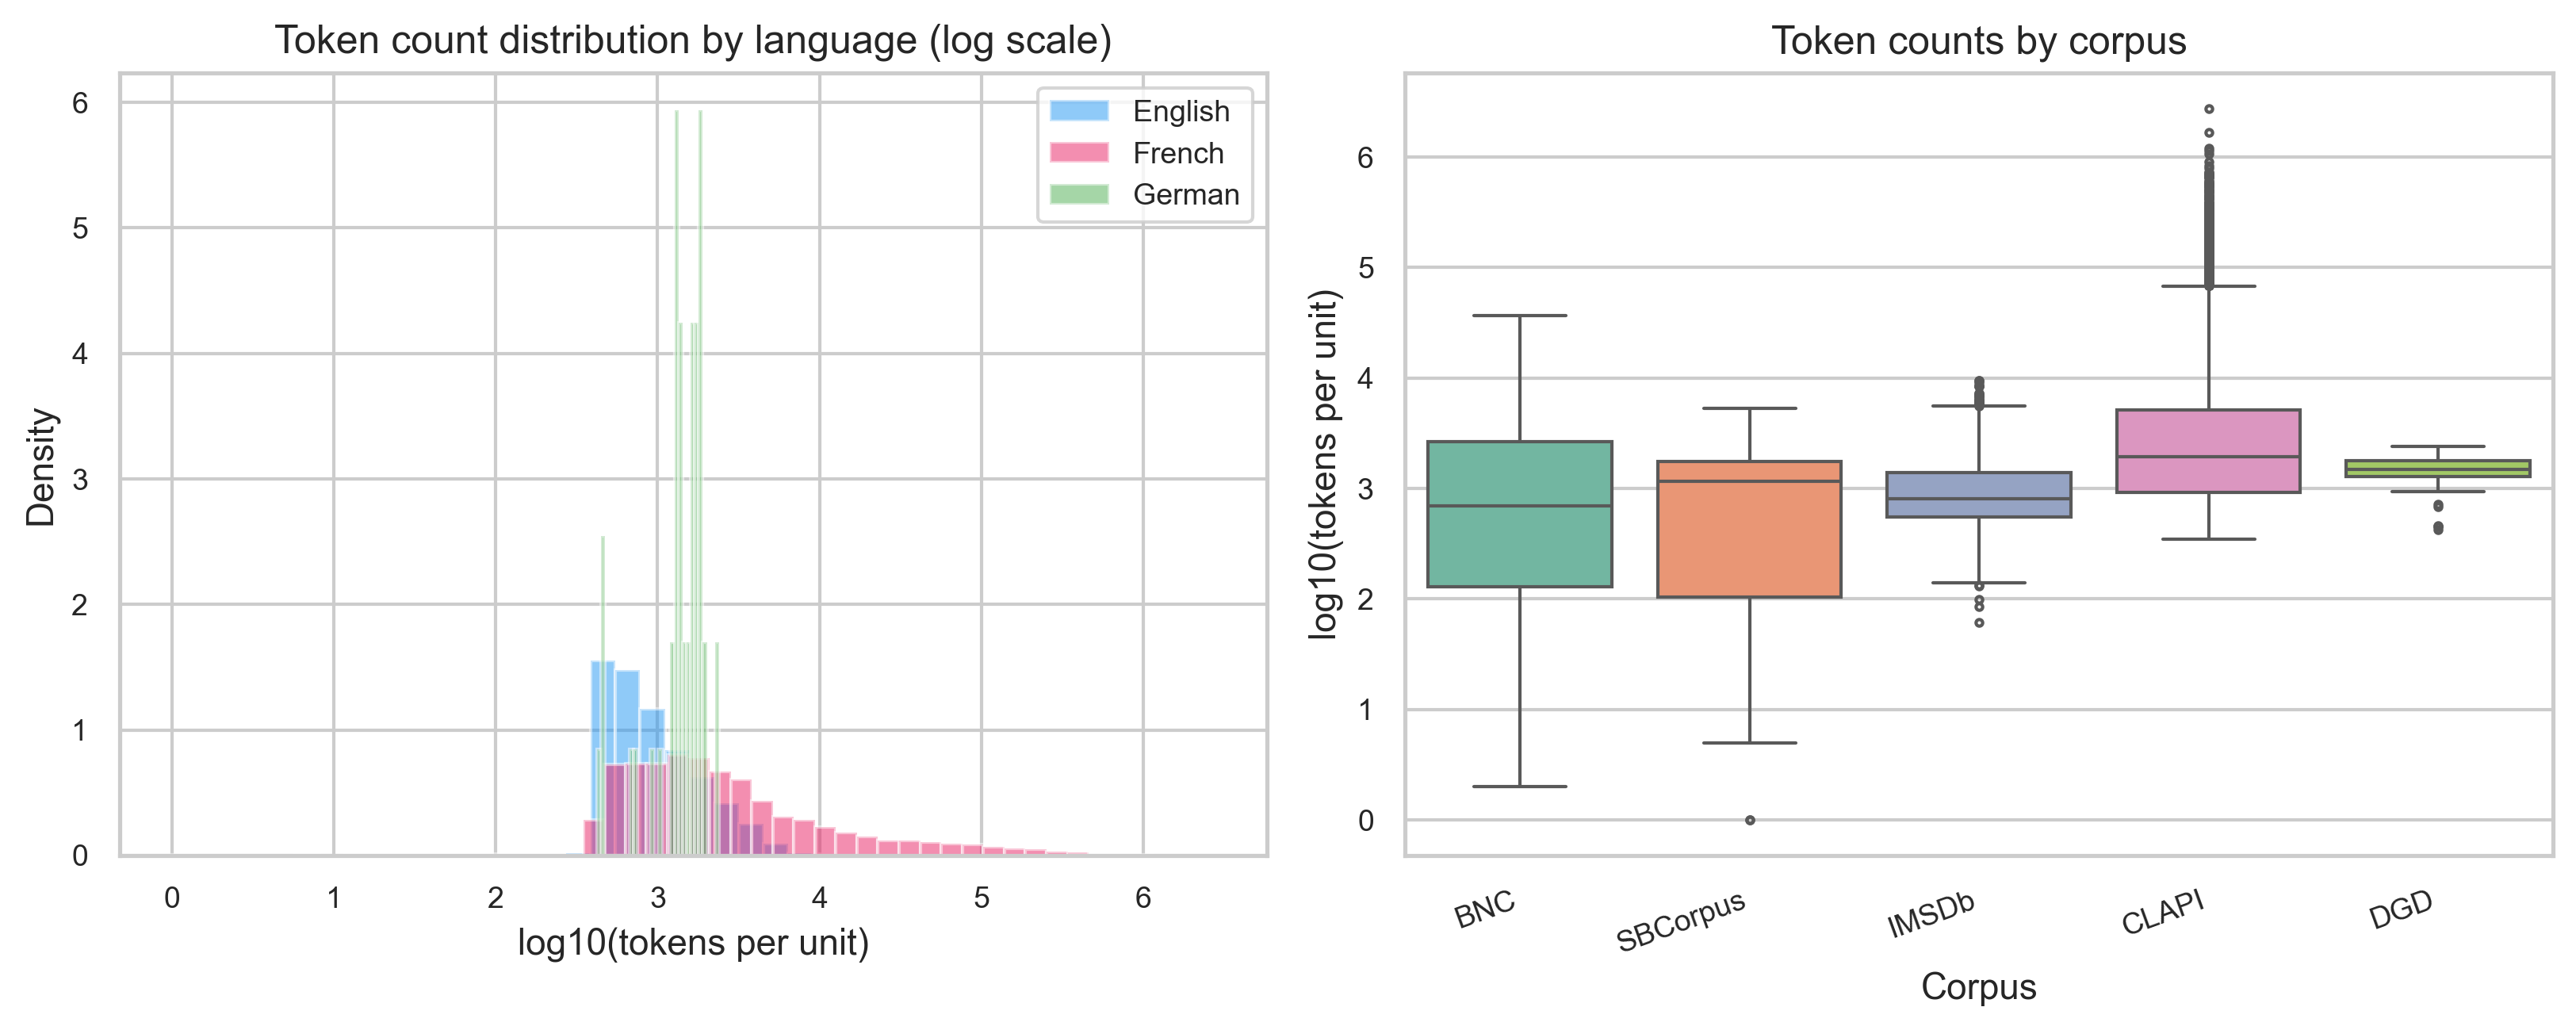
\includegraphics[width=\textwidth]{../results/figures/tokens_by_language.png}
    \caption{Distribution of token counts by language for the spoken/dialogue corpora.}
    \label{fig:results_tokens_by_language}
\end{figure}

\paragraph{Interpretation placeholder.}
TODO: Explain the sample-size structure across languages and why unequal token counts matter for richness estimation.

\begin{figure}[htbp]
    \centering
    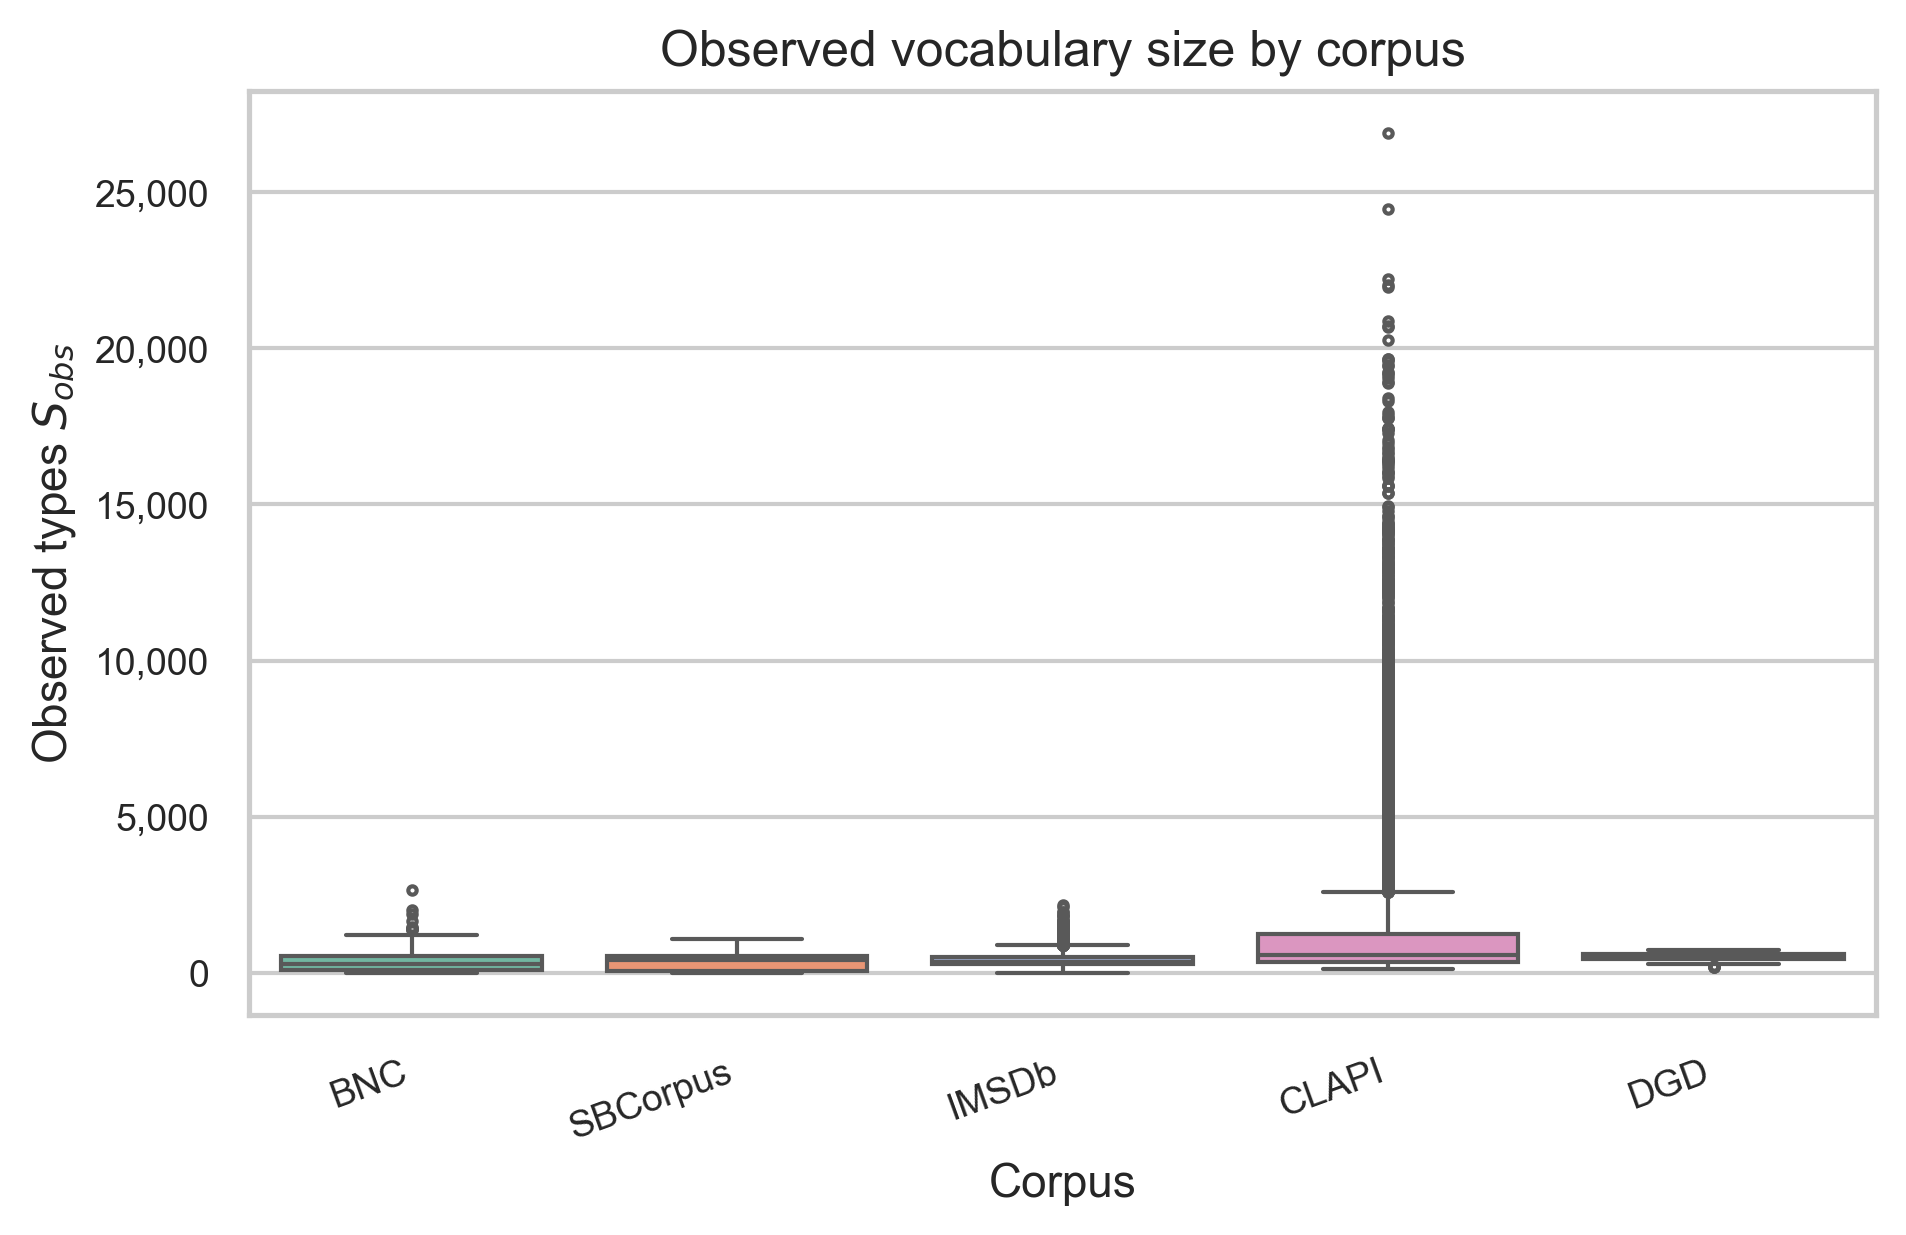
\includegraphics[width=\textwidth]{../results/figures/sobs_by_corpus.png}
    \caption{Observed vocabulary size by corpus.}
    \label{fig:results_sobs_by_corpus}
\end{figure}

\paragraph{Interpretation placeholder.}
TODO: Explain how observed vocabulary differs across corpora and why this should not yet be interpreted as total vocabulary richness.

\begin{figure}[htbp]
    \centering
    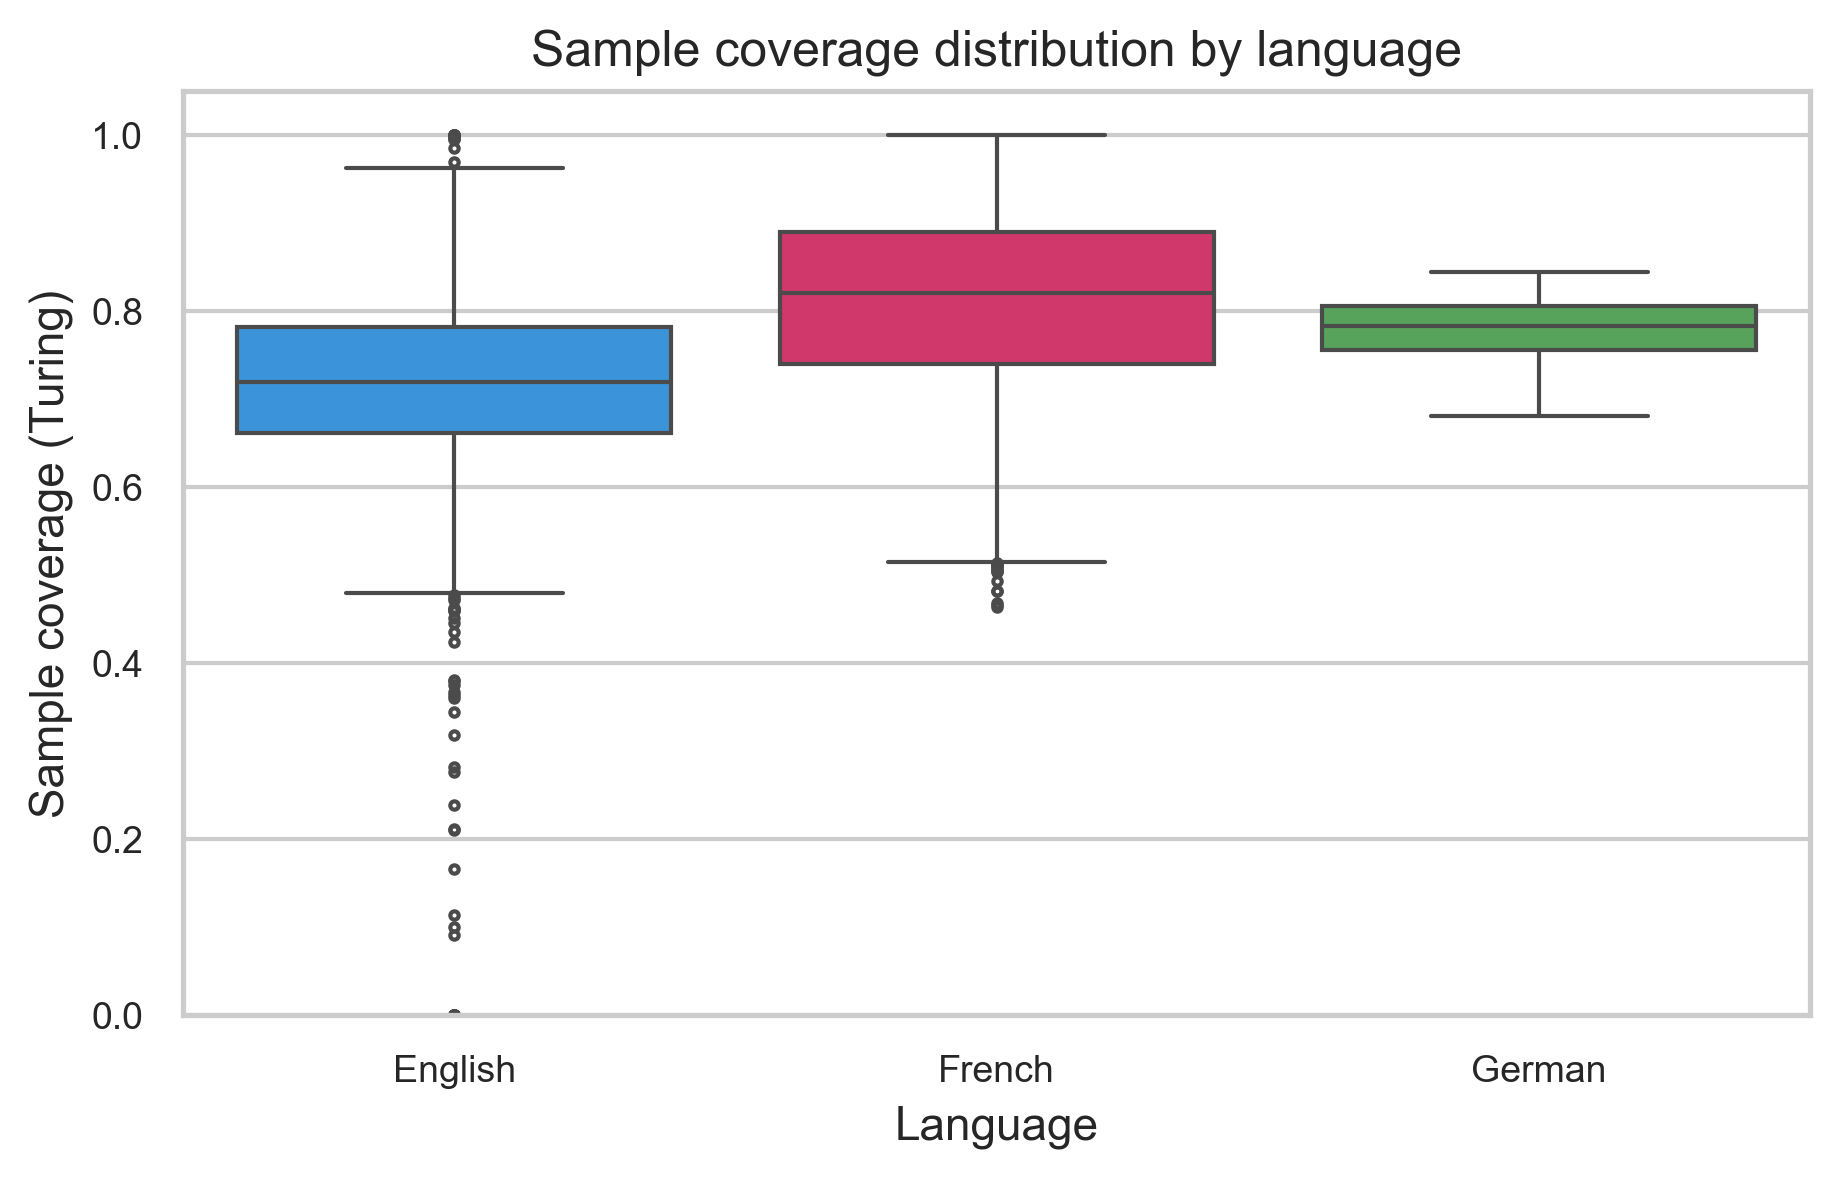
\includegraphics[width=\textwidth]{../results/figures/coverage_by_language.png}
    \caption{Sample coverage by language for the spoken/dialogue corpora.}
    \label{fig:results_coverage_by_language}
\end{figure}

\paragraph{Interpretation placeholder.}
TODO: Explain what the coverage values imply about sample completeness and estimator uncertainty.

\subsection{Per-language estimator results}

This section compares the richness estimates produced by the different estimators within each language.

\begin{table}[htbp]
    \centering
    \resizebox{\textwidth}{!}{
    \begin{tabular}{llrrrrr}
        Language & Estimator & Mean $\hat{S}$ & Median $\hat{S}$ & IQR $\hat{S}$ & Median $\hat{S}/S_{\mathrm{obs}}$ & Failed \\
        \hline
        English & Chao1 & 1015.4 & 885.9 & 546.6 & 2.3519 & 0 \\
        English & iChao1 & 1111.7 & 968.4 & 595.0 & 2.5719 & 0 \\
        English & ACE & 1771.5 & 1523.0 & 994.7 & 4.0940 & 10 \\
        English & Jackknife1 & 694.8 & 585.6 & 378.7 & 1.6352 & 0 \\
        English & Jackknife2 & 901.2 & 764.7 & 486.2 & 2.1257 & 2 \\
        English & Breakaway & 3320.0 & 1927.2 & 1880.0 & 5.2128 & 2764 \\
        French & Chao1 & 2721.7 & 1377.2 & 1968.9 & 2.1066 & 0 \\
        French & iChao1 & 2960.7 & 1507.5 & 2155.8 & 2.3069 & 0 \\
        French & ACE & 4990.2 & 2443.5 & 3514.4 & 3.8163 & 0 \\
        French & Jackknife1 & 2155.6 & 928.8 & 1400.0 & 1.5676 & 0 \\
        French & Jackknife2 & 2677.4 & 1200.7 & 1806.1 & 2.0035 & 0 \\
        French & Breakaway & 22309.1 & 3249.9 & 7208.9 & 4.9321 & 5516 \\
        German & Chao1 & 1163.3 & 1269.4 & 406.5 & 2.2451 & 0 \\
        German & iChao1 & 1269.6 & 1359.3 & 438.1 & 2.4446 & 0 \\
        German & ACE & 2075.6 & 2188.3 & 811.5 & 4.0295 & 0 \\
        German & Jackknife1 & 808.8 & 855.8 & 227.5 & 1.6027 & 0 \\
        German & Jackknife2 & 1045.6 & 1111.3 & 312.8 & 2.0642 & 0 \\
        German & Breakaway & 5746.8 & 2500.3 & 2619.9 & 5.2887 & 20 \\
    \end{tabular}}
    \caption{Per-language estimator summary for the spoken/dialogue corpora.}
    \label{tab:results_per_language_estimator_summary}
\end{table}

\paragraph{Table interpretation placeholder.}
TODO: Explain the per-language estimator table, including the large Breakaway failure counts.

\begin{figure}[htbp]
    \centering
    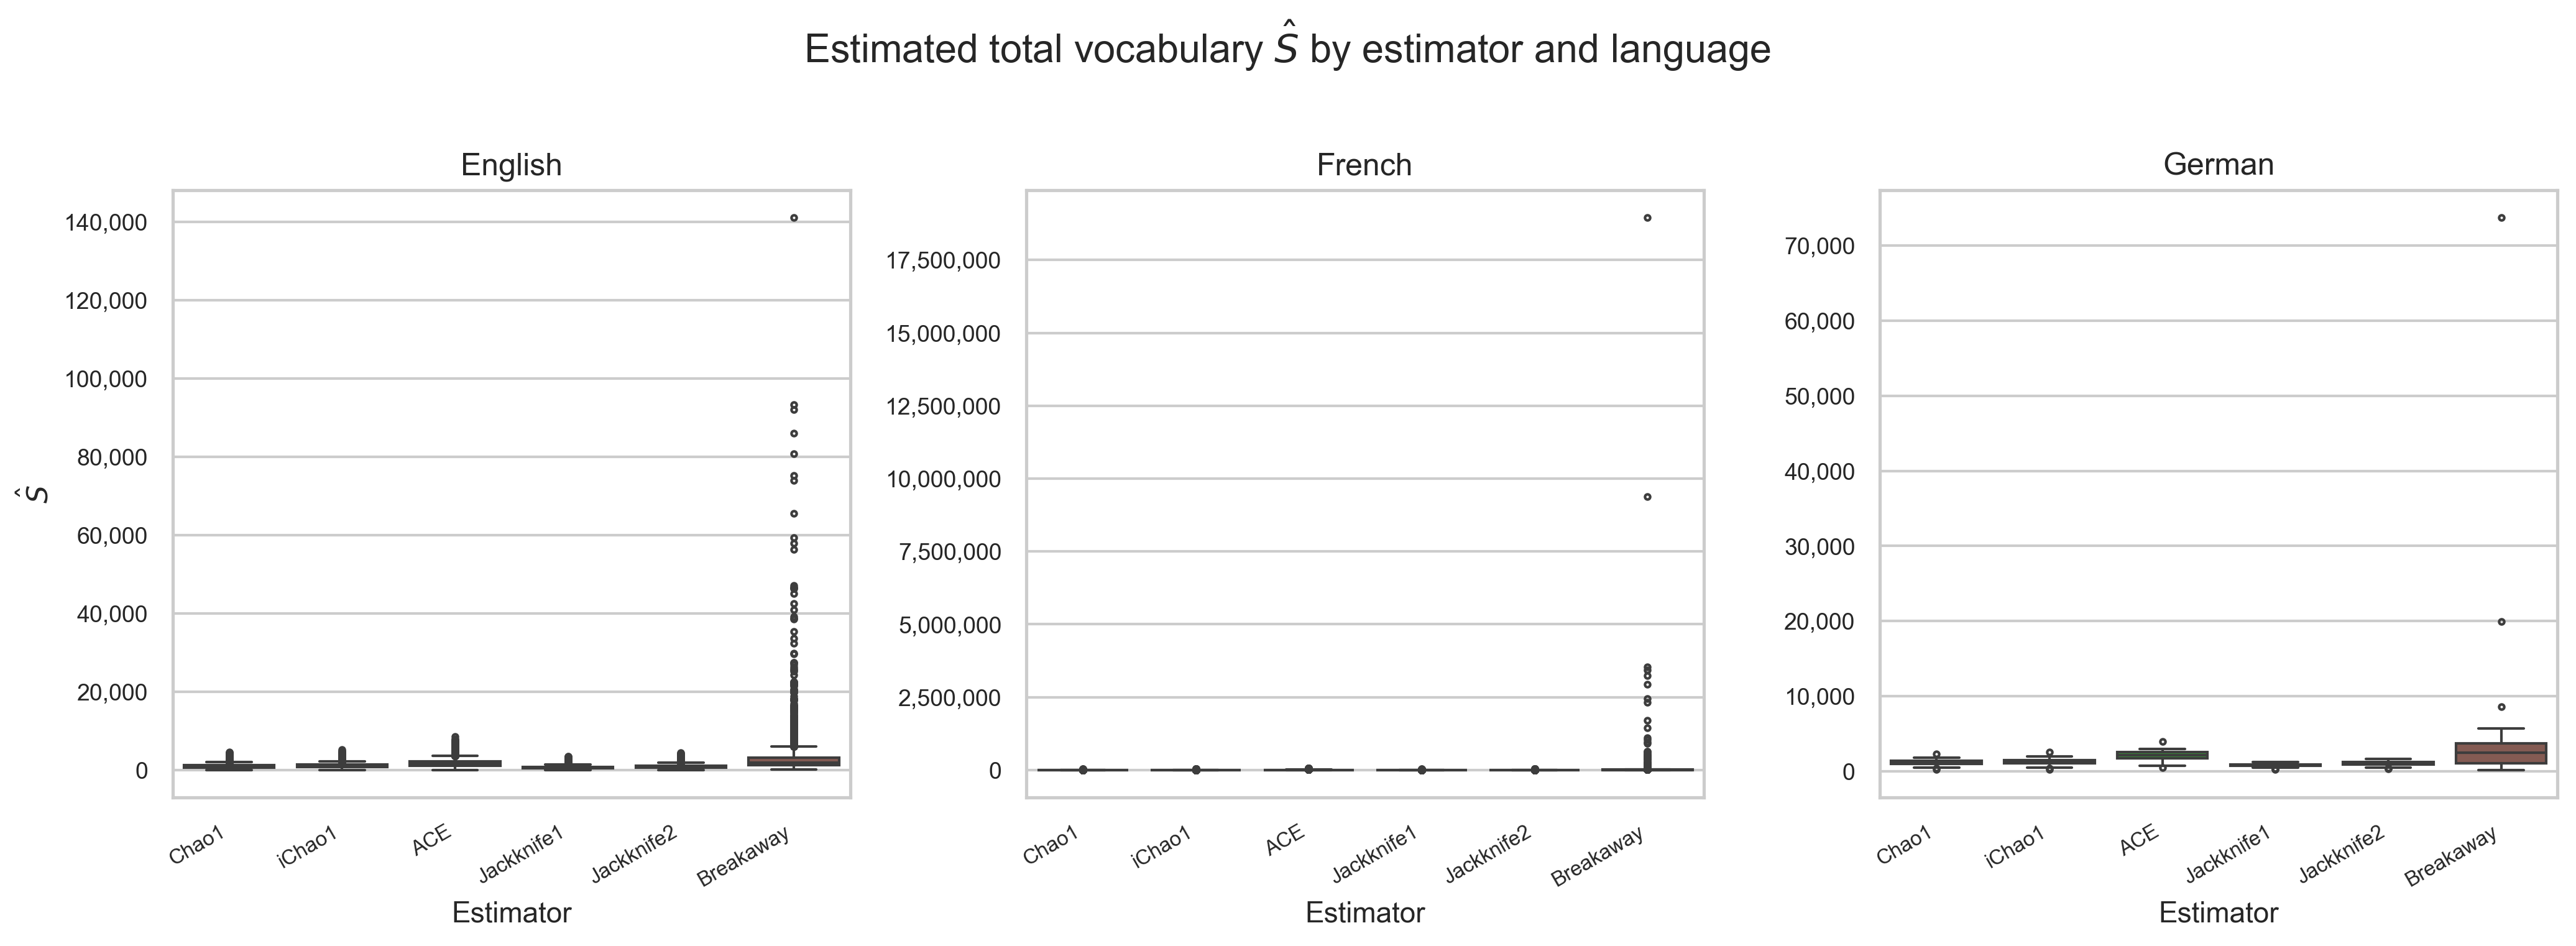
\includegraphics[width=\textwidth]{../results/figures/estimator_boxplots_by_language.png}
    \caption{Distribution of estimated richness by estimator and language.}
    \label{fig:results_estimator_boxplots_by_language}
\end{figure}

\paragraph{Interpretation placeholder.}
TODO: Explain which estimators give similar estimates, which ones diverge, and whether the divergence differs by language.

\begin{figure}[htbp]
    \centering
    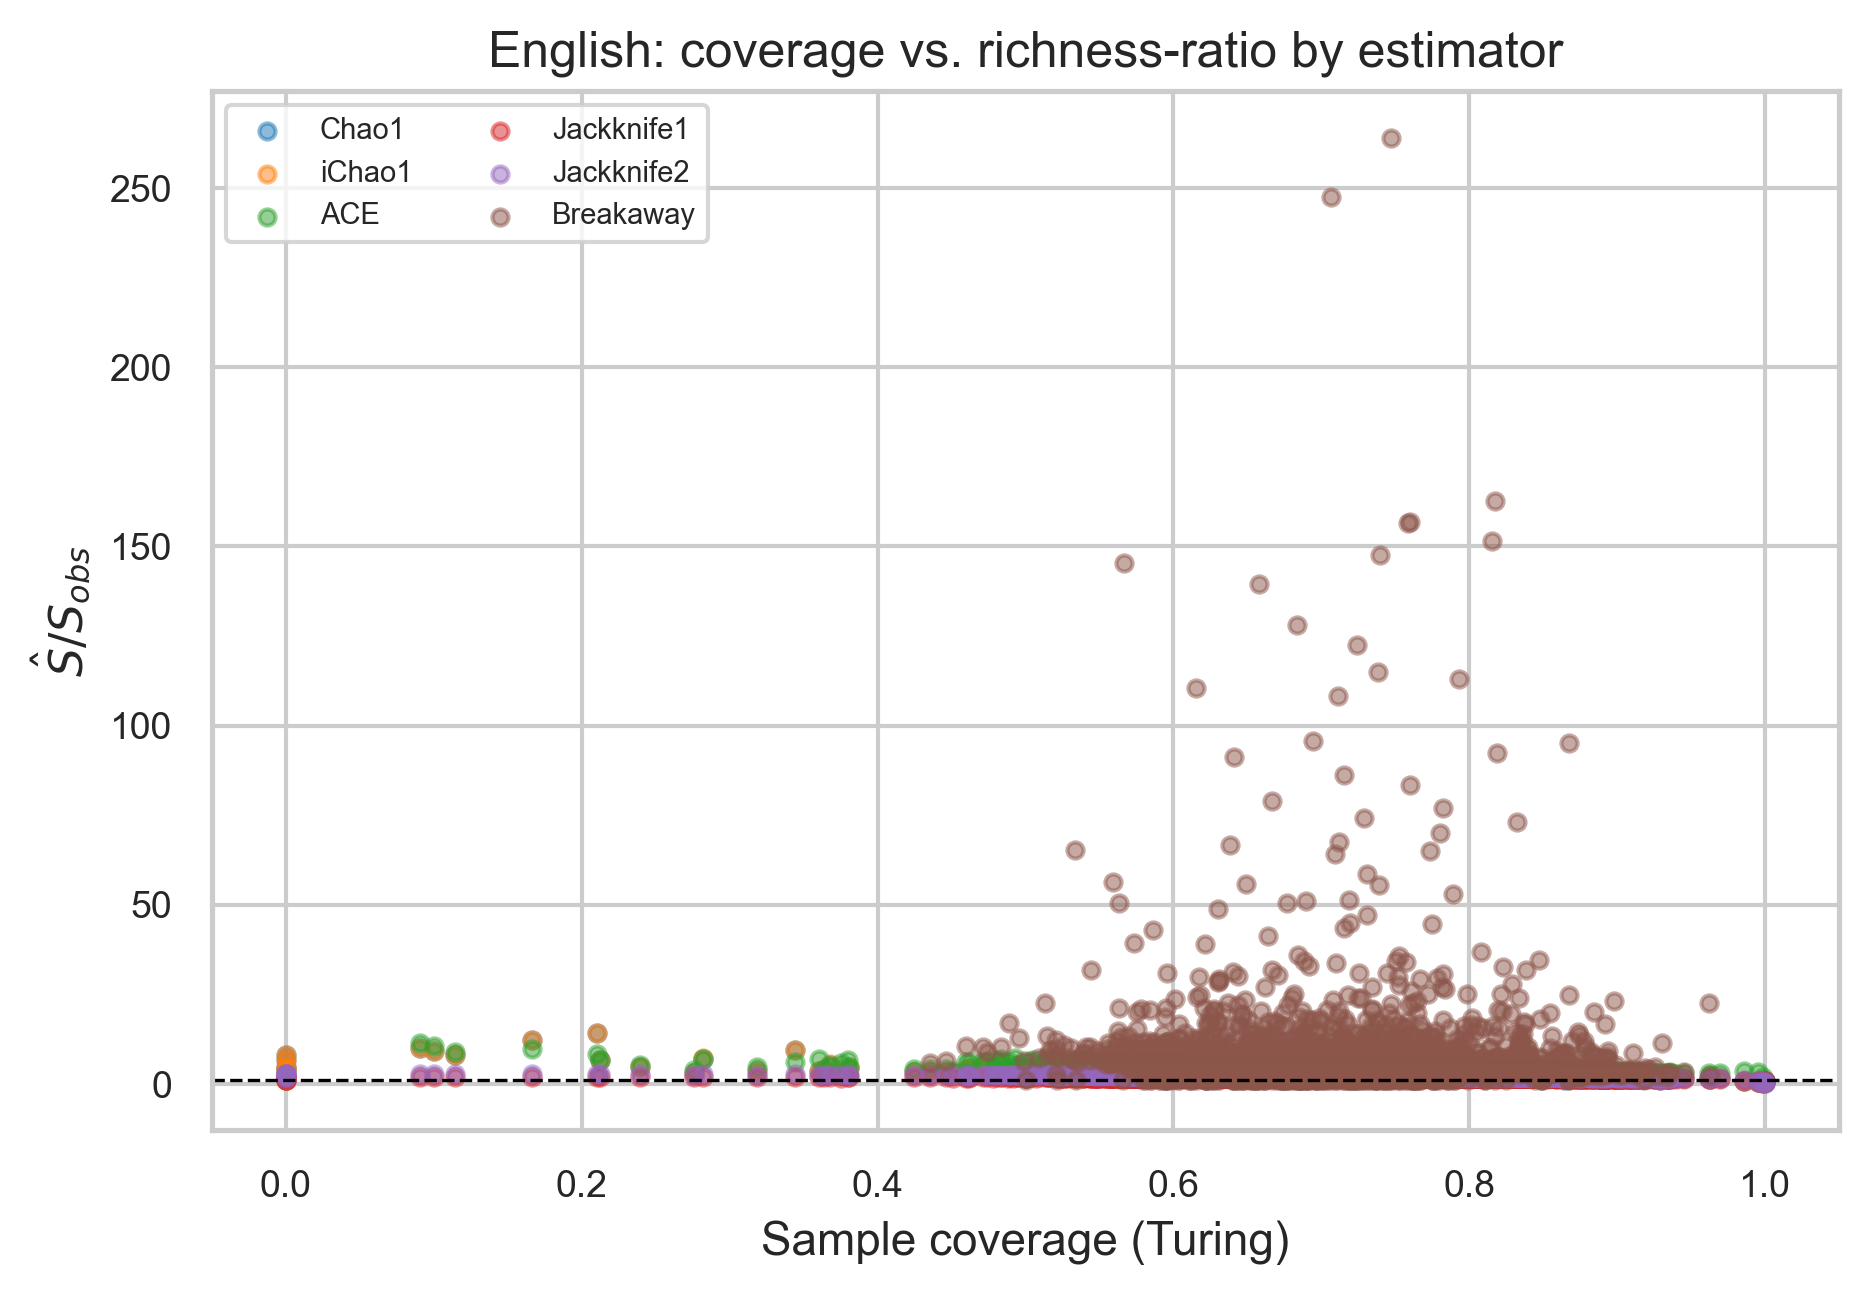
\includegraphics[width=\textwidth]{../results/figures/coverage_vs_ratio_english.png}
    \caption{Coverage versus estimated-to-observed richness ratio for English spoken/dialogue corpora.}
    \label{fig:results_coverage_vs_ratio_english}
\end{figure}

\paragraph{Interpretation placeholder.}
TODO: Explain how estimator extrapolation changes with coverage for English.

\begin{figure}[htbp]
    \centering
    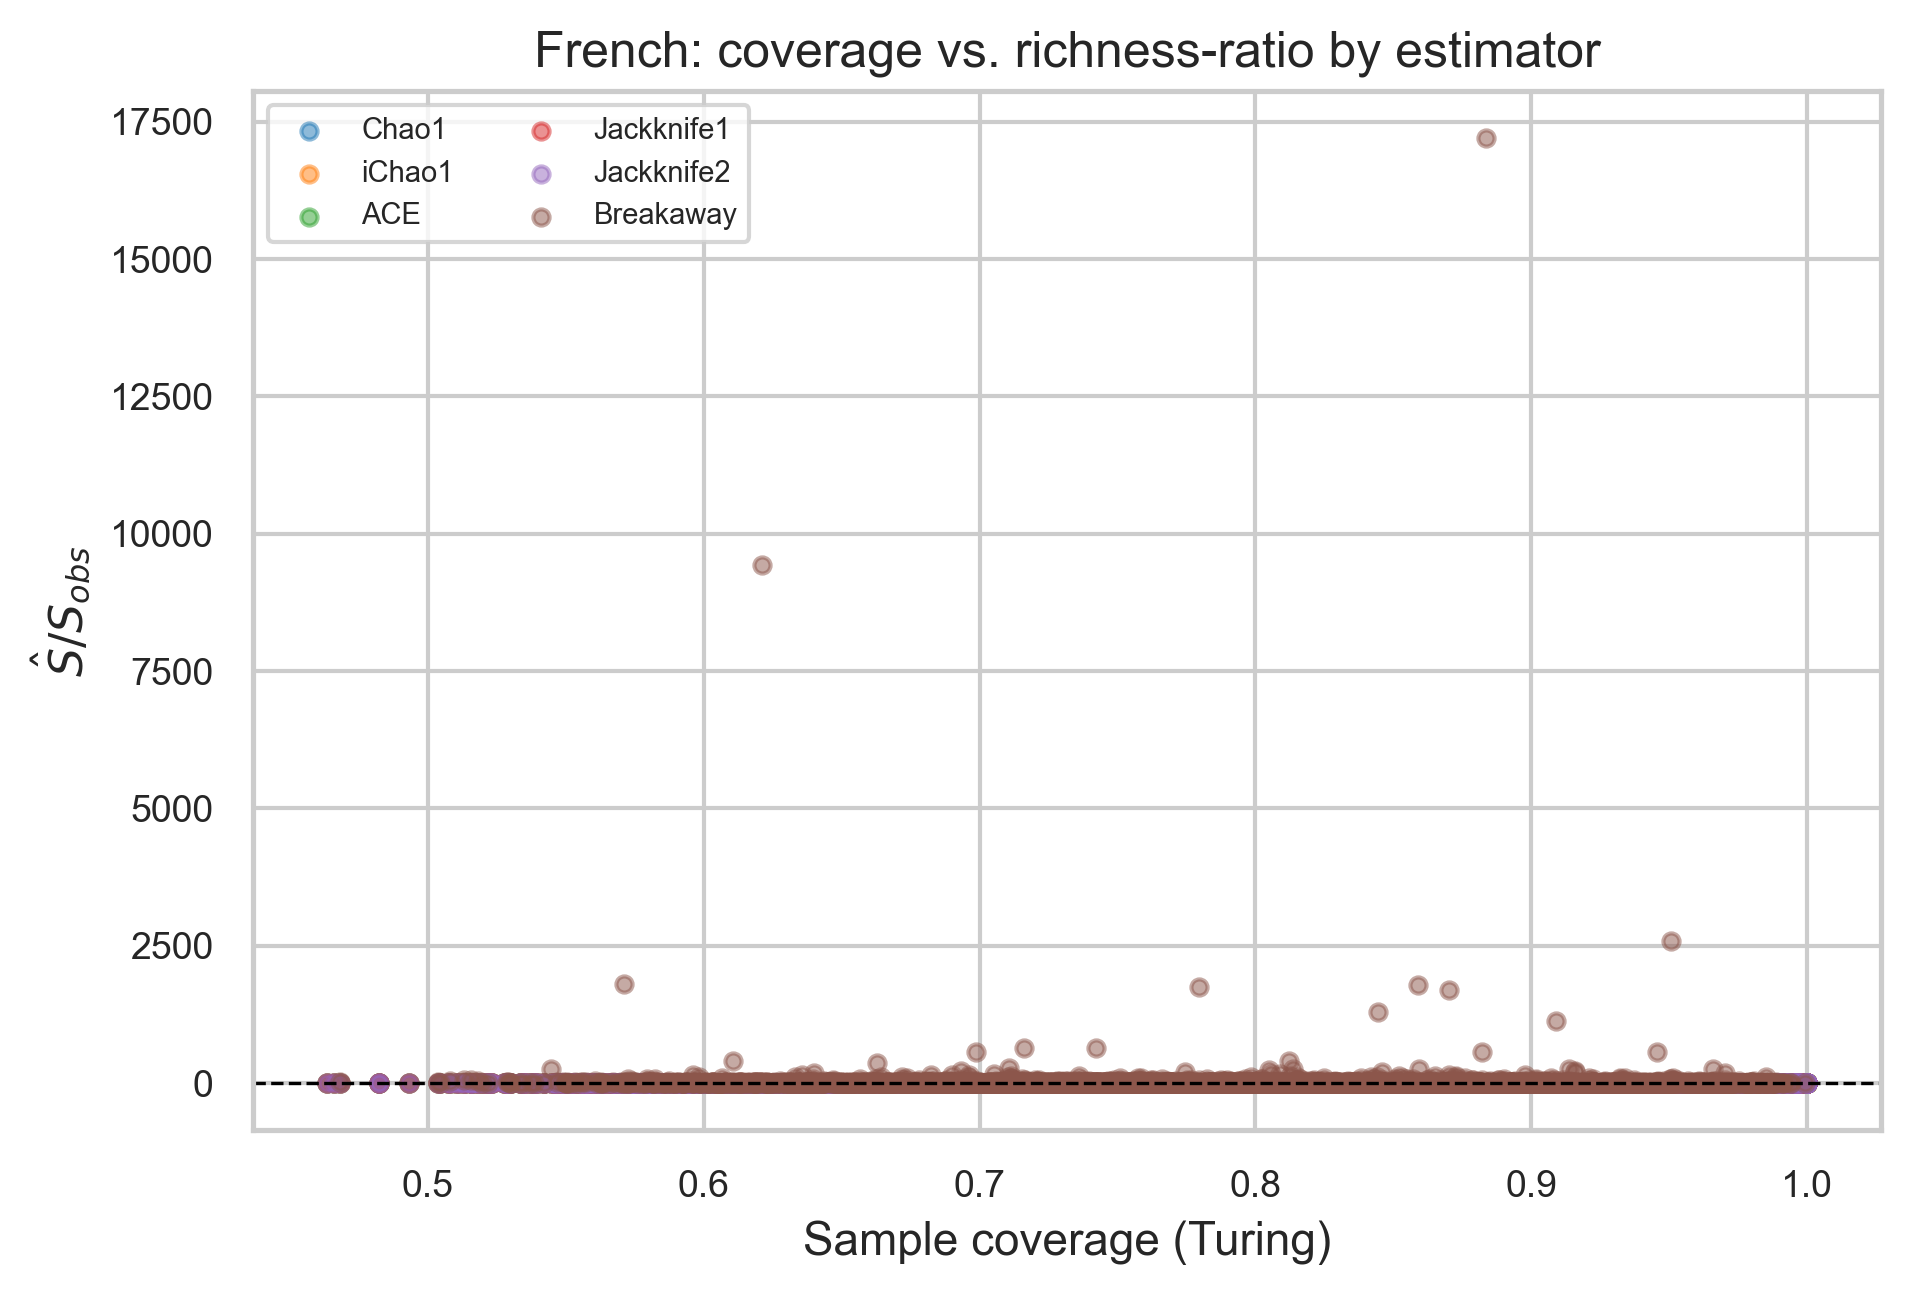
\includegraphics[width=\textwidth]{../results/figures/coverage_vs_ratio_french.png}
    \caption{Coverage versus estimated-to-observed richness ratio for the French spoken corpus.}
    \label{fig:results_coverage_vs_ratio_french}
\end{figure}

\paragraph{Interpretation placeholder.}
TODO: Explain how estimator extrapolation changes with coverage for French.

\begin{figure}[htbp]
    \centering
    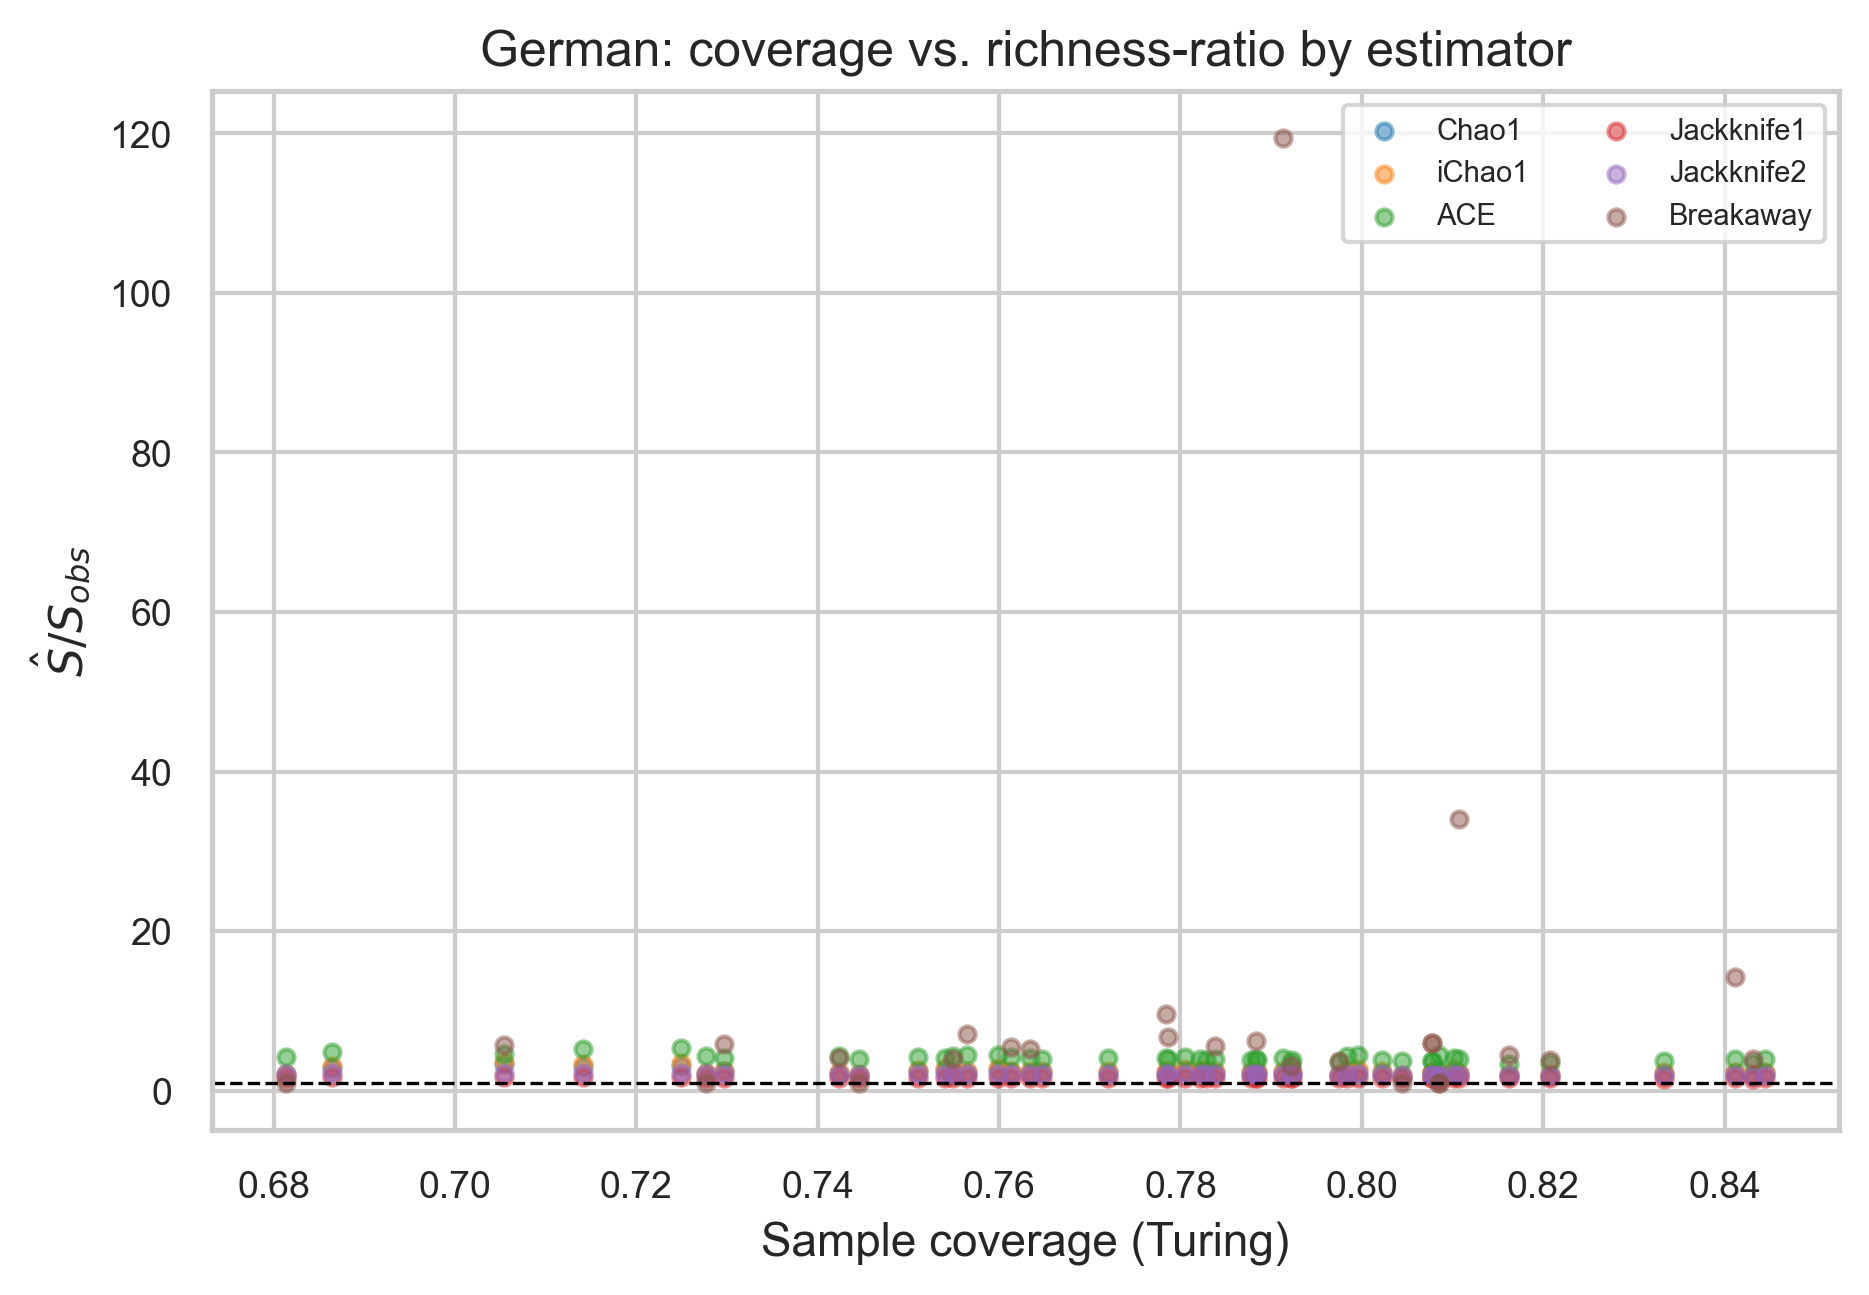
\includegraphics[width=\textwidth]{../results/figures/coverage_vs_ratio_german.png}
    \caption{Coverage versus estimated-to-observed richness ratio for the German spoken corpus.}
    \label{fig:results_coverage_vs_ratio_german}
\end{figure}

\paragraph{Interpretation placeholder.}
TODO: Explain how estimator extrapolation changes with coverage for German.

\subsection{Completely monotone and k-monotone model selection}

The following figures document how the finite-$k$ and completely monotone shape-constrained estimates behave. These results should be interpreted as empirical support for, or against, using the completely monotone limit.

\begin{table}[htbp]
    \centering
    \resizebox{\textwidth}{!}{
    \begin{tabular}{lrrrrr}
        Language/Corpus & Units & Median $k^\ast$ & Mean $k^\ast$ & $k^\ast = k_{\max}$ (\%) & Median $\hat{S}_{CM}$ \\
        \hline
        English & 15 & 5.0 & 5.0 & 0.0 & 1707.0 \\
        French & 15 & 6.0 & 6.0 & 0.0 & 17525.0 \\
        German & 15 & 4.0 & 4.1 & 0.0 & 605.0 \\
        Shakespeare & 43 & 8.0 & 7.3 & 0.0 & 3390.0 \\
    \end{tabular}}
    \caption{Summary of selected finite-$k$ monotone and completely monotone estimates. The full selection table is stored in \texttt{results/tables/cm\_kmonotone\_selection.csv}.}
    \label{tab:results_cm_kmonotone_summary}
\end{table}

\paragraph{Table interpretation placeholder.}
TODO: Explain whether the selected $k$ values support using the completely monotone limit.

\begin{figure}[htbp]
    \centering
    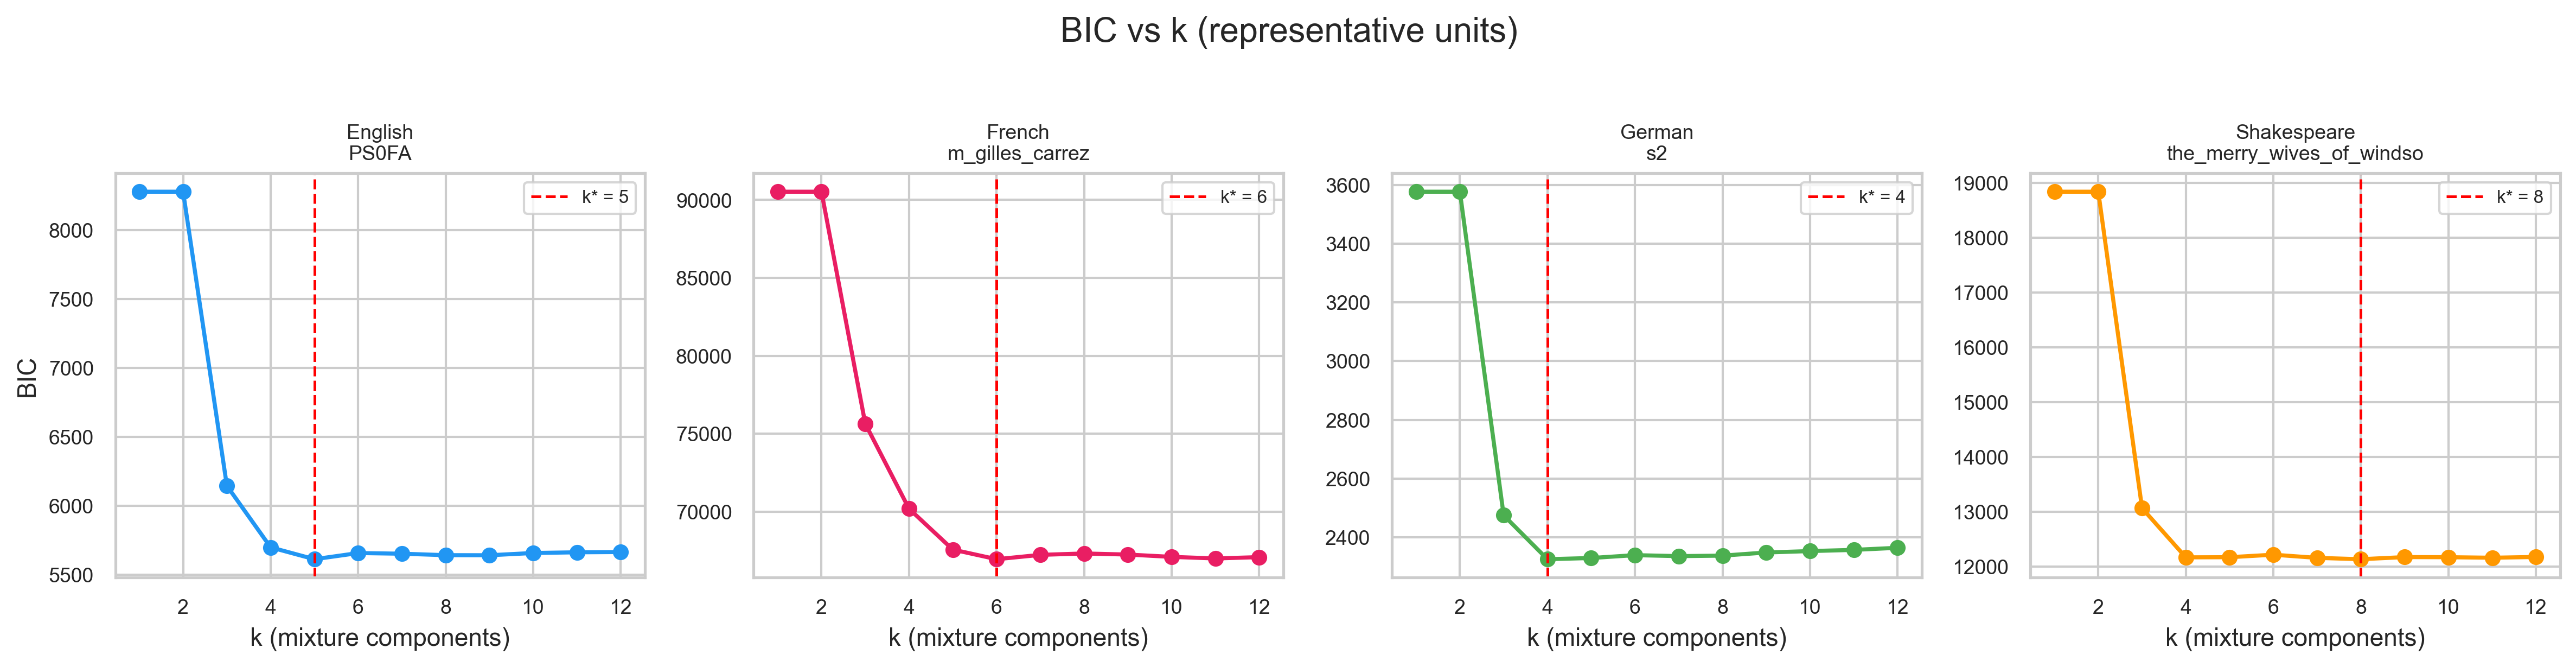
\includegraphics[width=\textwidth]{../results/figures/cm_k_selection_bic.png}
    \caption{BIC values across candidate values of $k$ for representative units.}
    \label{fig:results_cm_k_selection_bic}
\end{figure}

\paragraph{Interpretation placeholder.}
TODO: Explain where the BIC minimum occurs and whether the selected $k$ values suggest low-order or high-order monotonicity.

\begin{figure}[htbp]
    \centering
    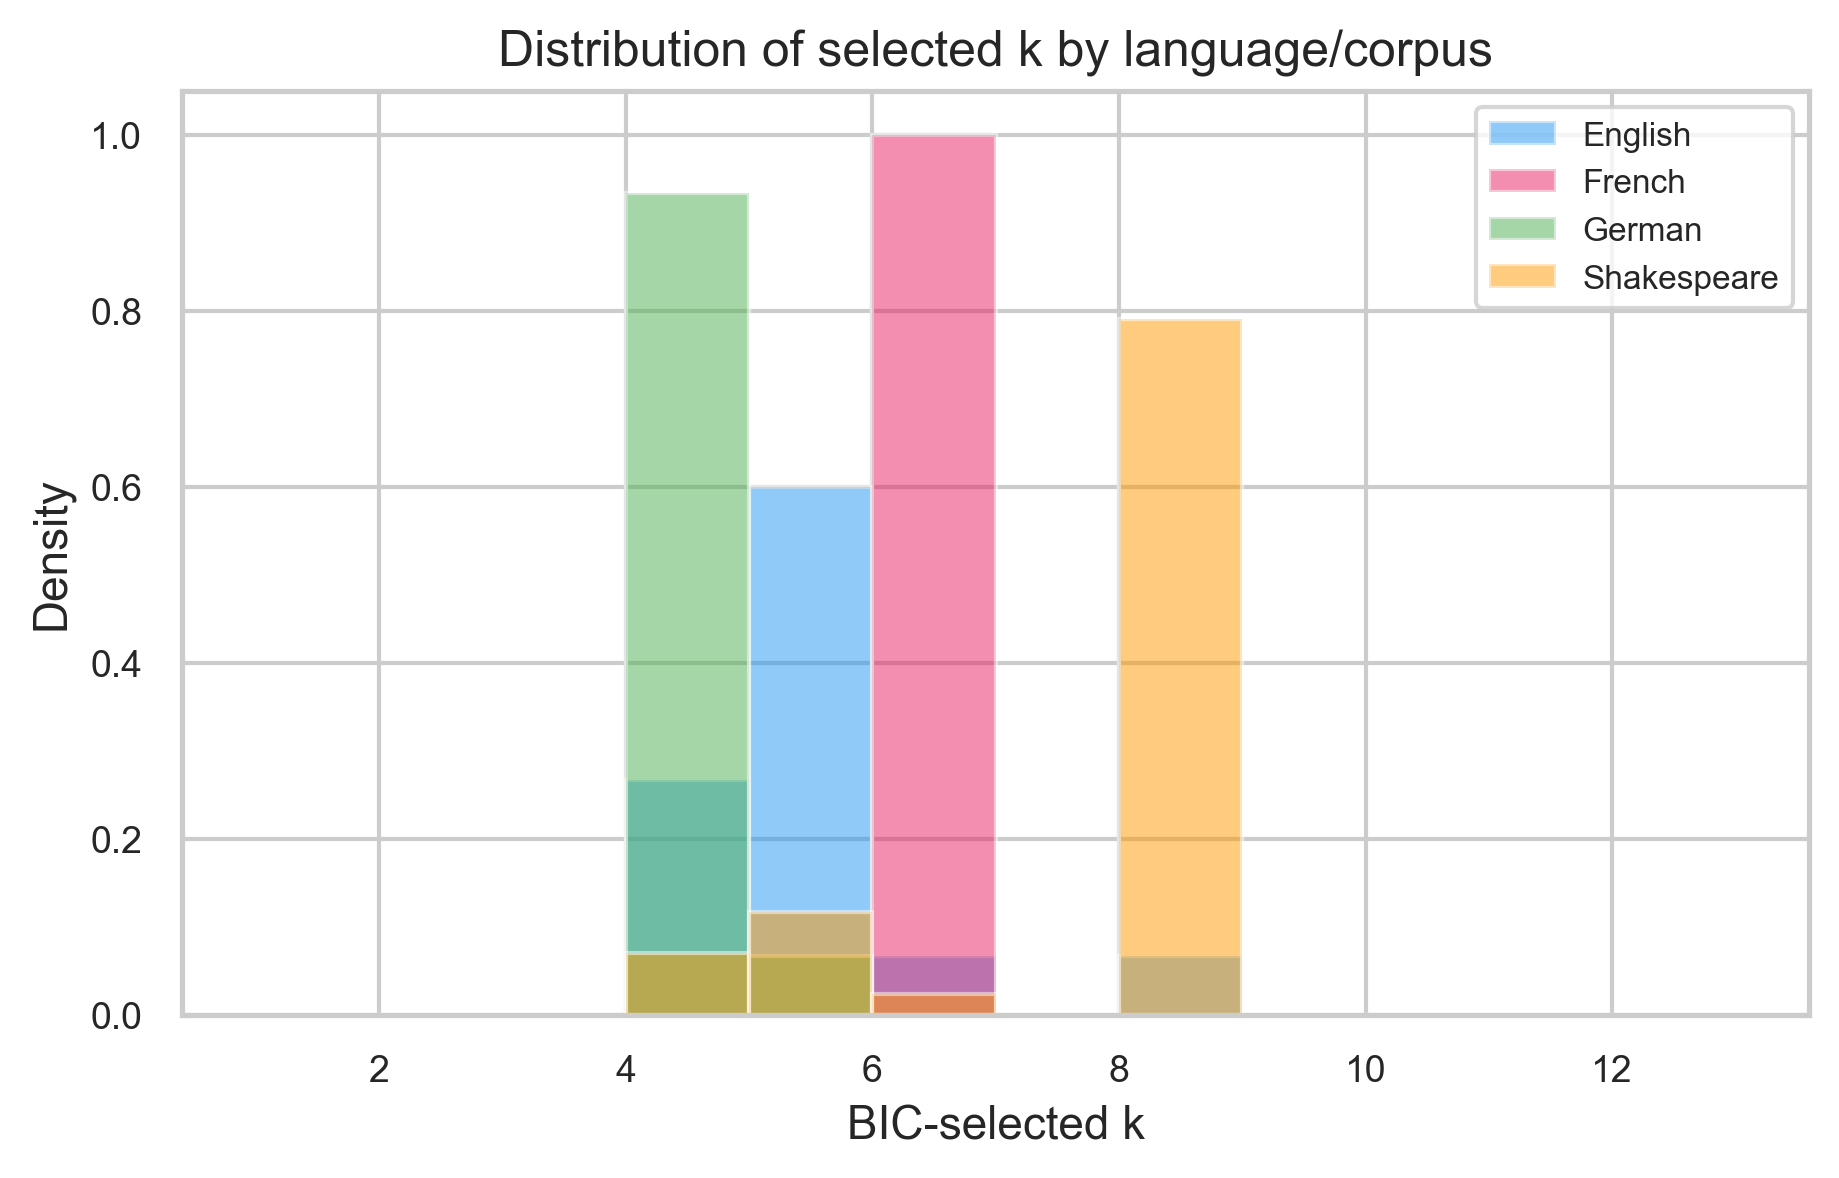
\includegraphics[width=\textwidth]{../results/figures/cm_k_selection_histogram.png}
    \caption{Distribution of selected $k$ values across corpora and languages.}
    \label{fig:results_cm_k_selection_histogram}
\end{figure}

\paragraph{Interpretation placeholder.}
TODO: Explain whether selected $k$ values concentrate near the maximum tested value or remain small.

\begin{figure}[htbp]
    \centering
    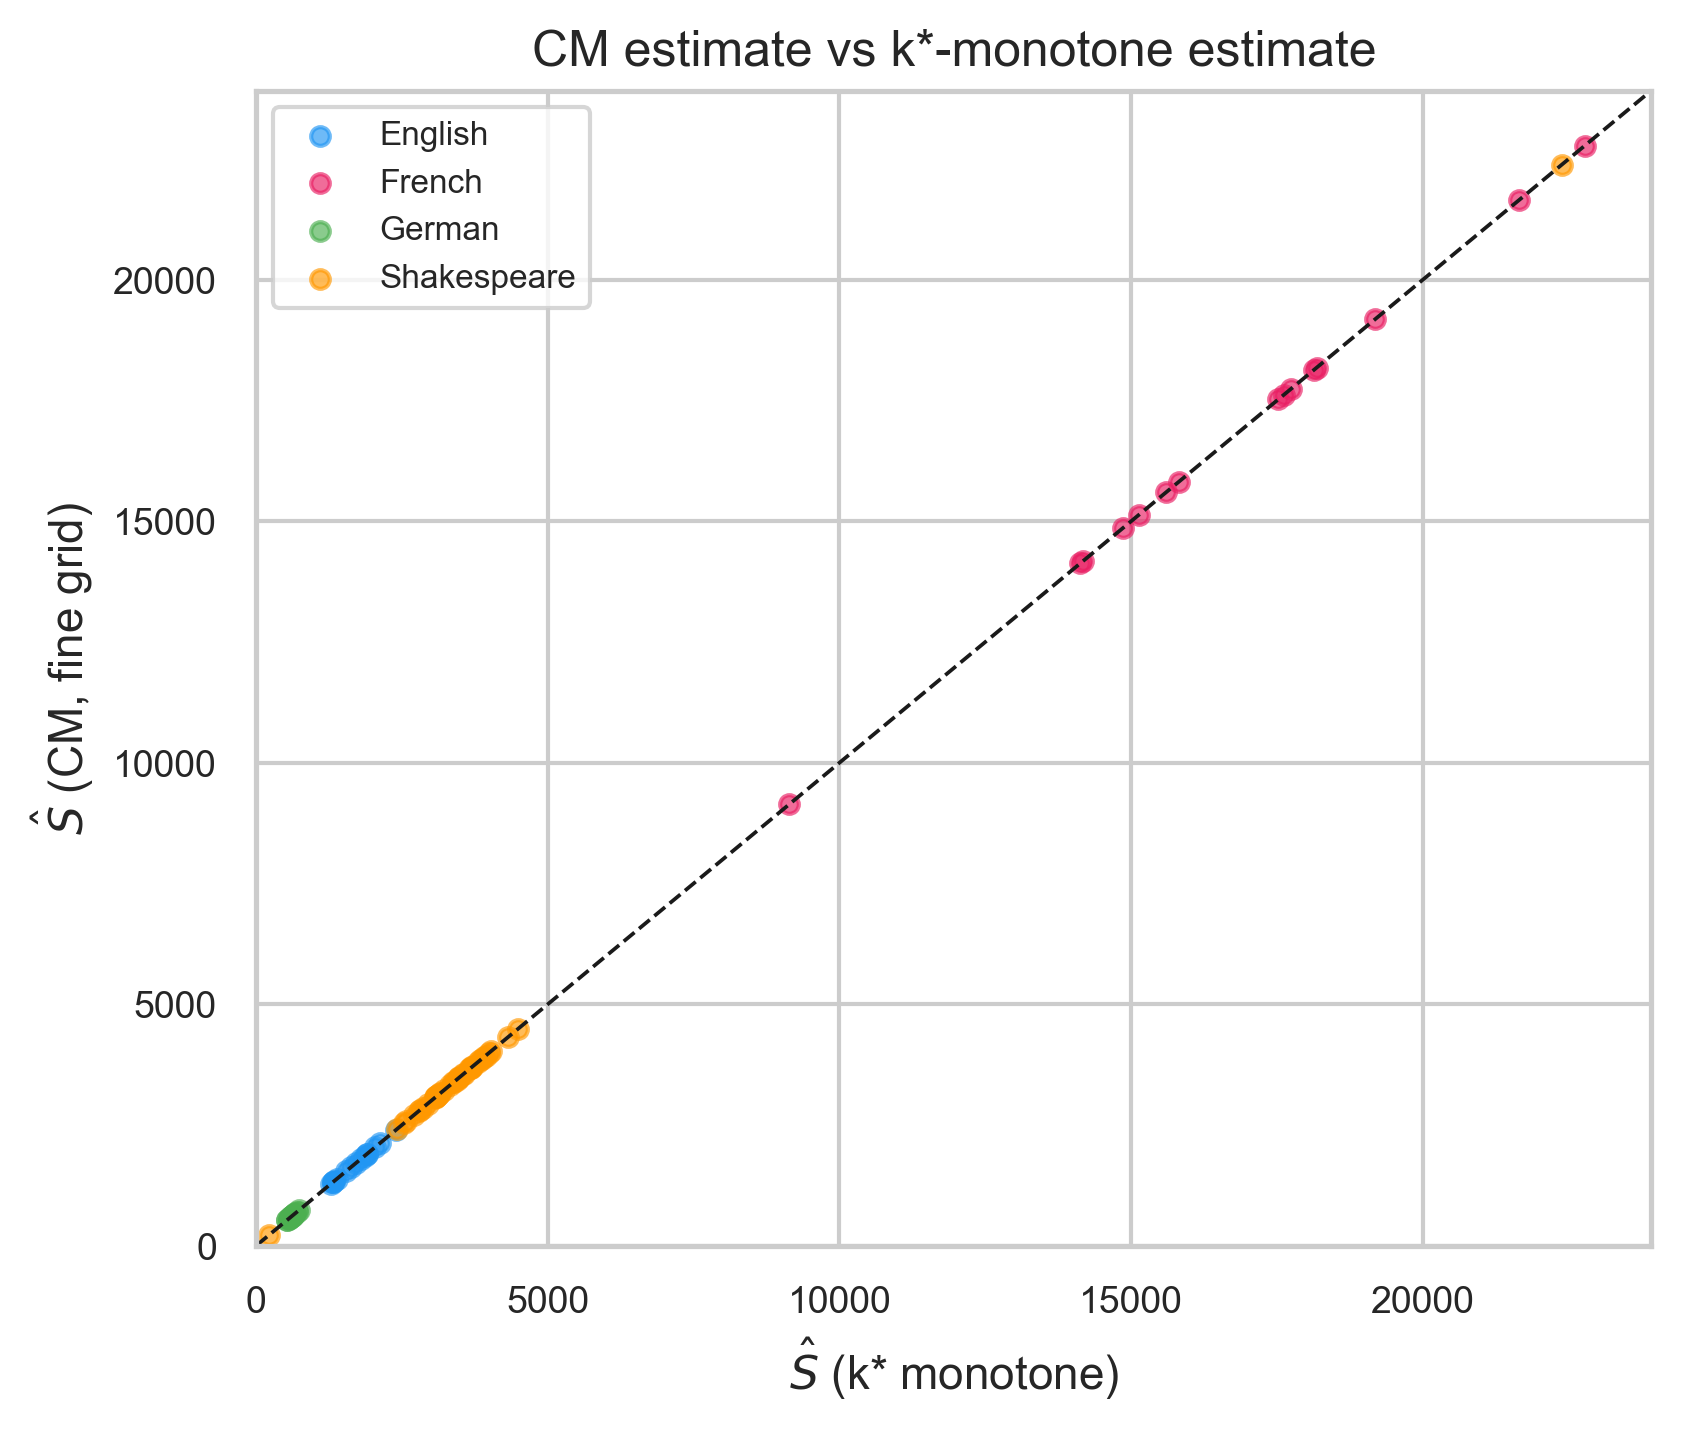
\includegraphics[width=\textwidth]{../results/figures/cm_vs_kmonotone_scatter.png}
    \caption{Comparison between completely monotone estimates and selected finite-$k$ monotone estimates.}
    \label{fig:results_cm_vs_kmonotone_scatter}
\end{figure}

\paragraph{Interpretation placeholder.}
TODO: Explain whether the completely monotone and finite-$k$ estimates agree, and what disagreement would imply.

\subsection{Rarefaction and extrapolation}

Rarefaction and extrapolation curves show how observed vocabulary grows with sampling effort and how much additional vocabulary is expected beyond the observed sample.

\begin{figure}[htbp]
    \centering
    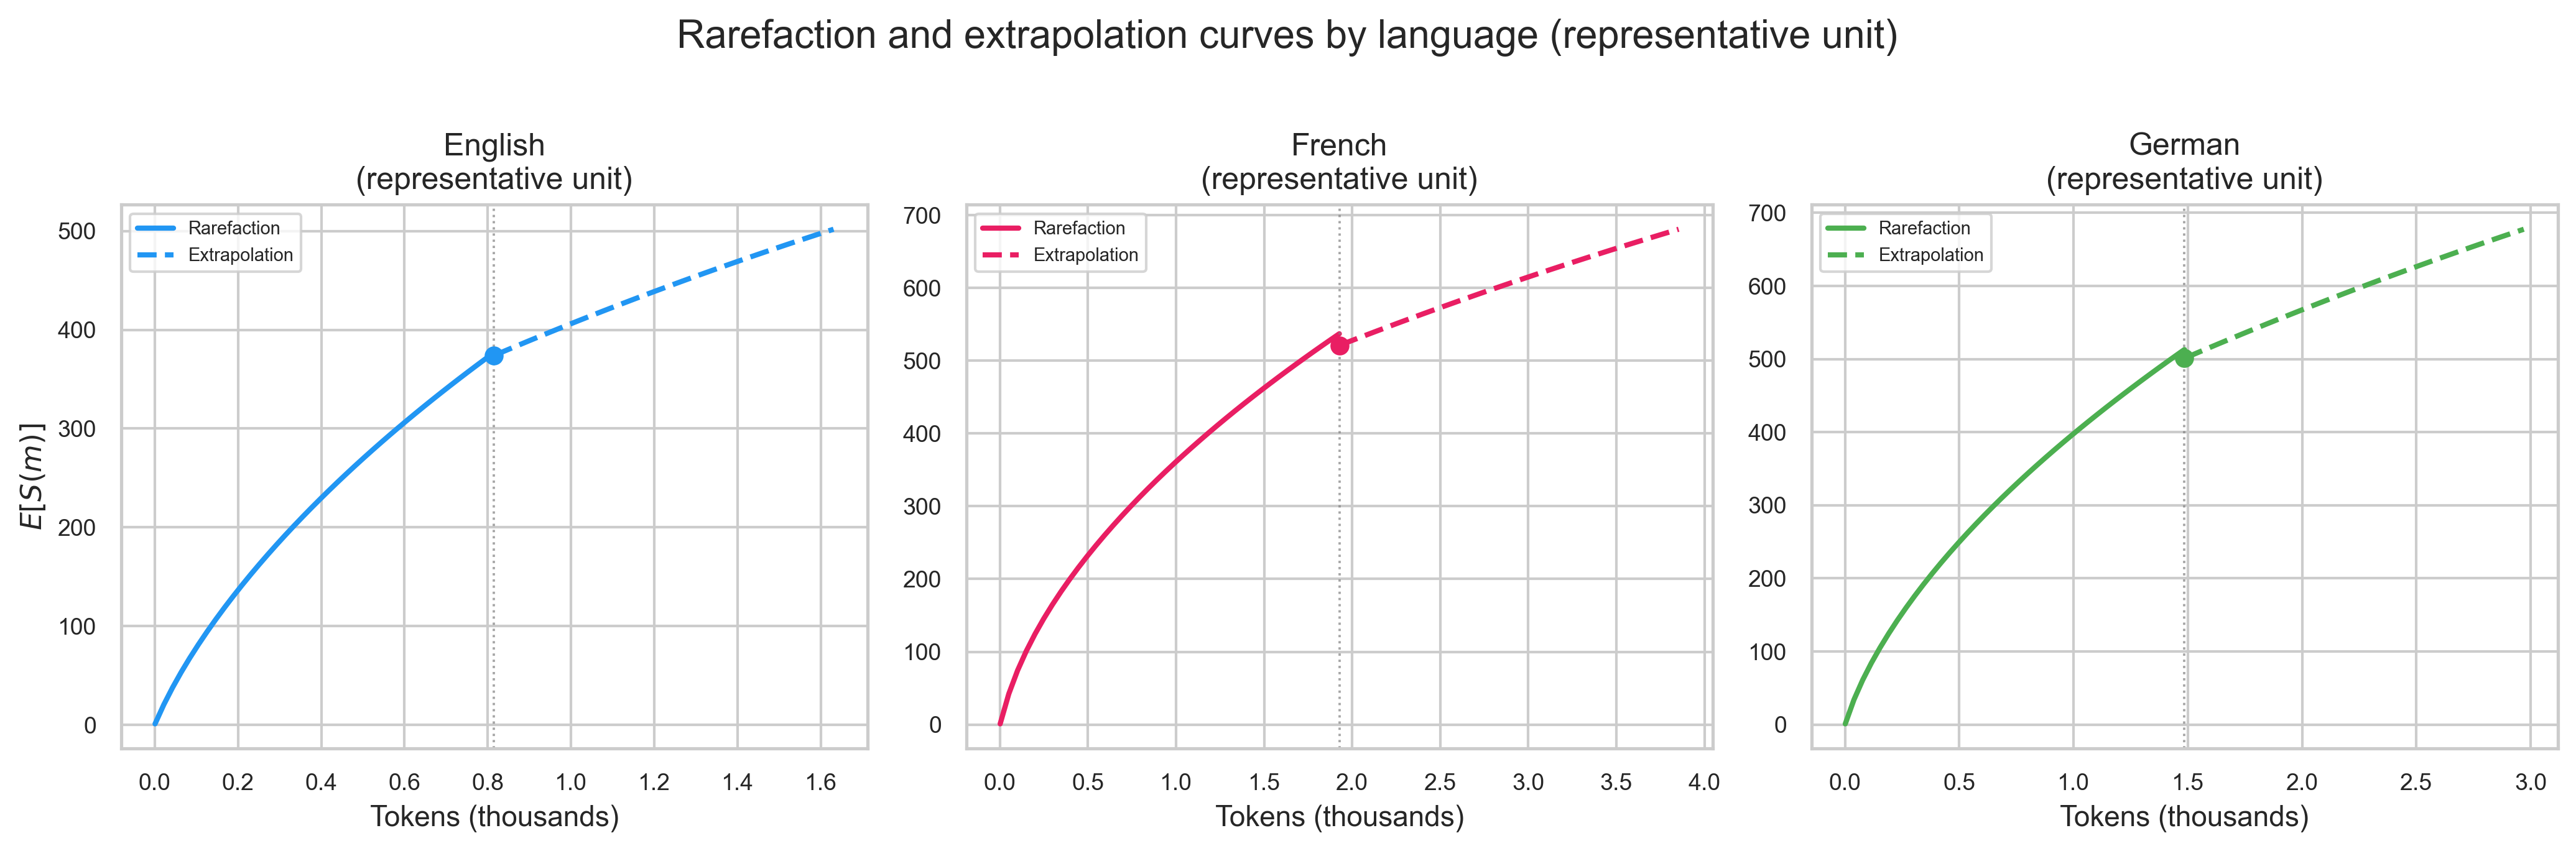
\includegraphics[width=\textwidth]{../results/figures/rarefaction_extrapolation_by_language.png}
    \caption{Rarefaction and extrapolation curves for representative spoken/dialogue units in each language.}
    \label{fig:results_rarefaction_extrapolation_by_language}
\end{figure}

\paragraph{Interpretation placeholder.}
TODO: Explain whether the representative language curves are close to saturation or still rising strongly.

\begin{figure}[htbp]
    \centering
    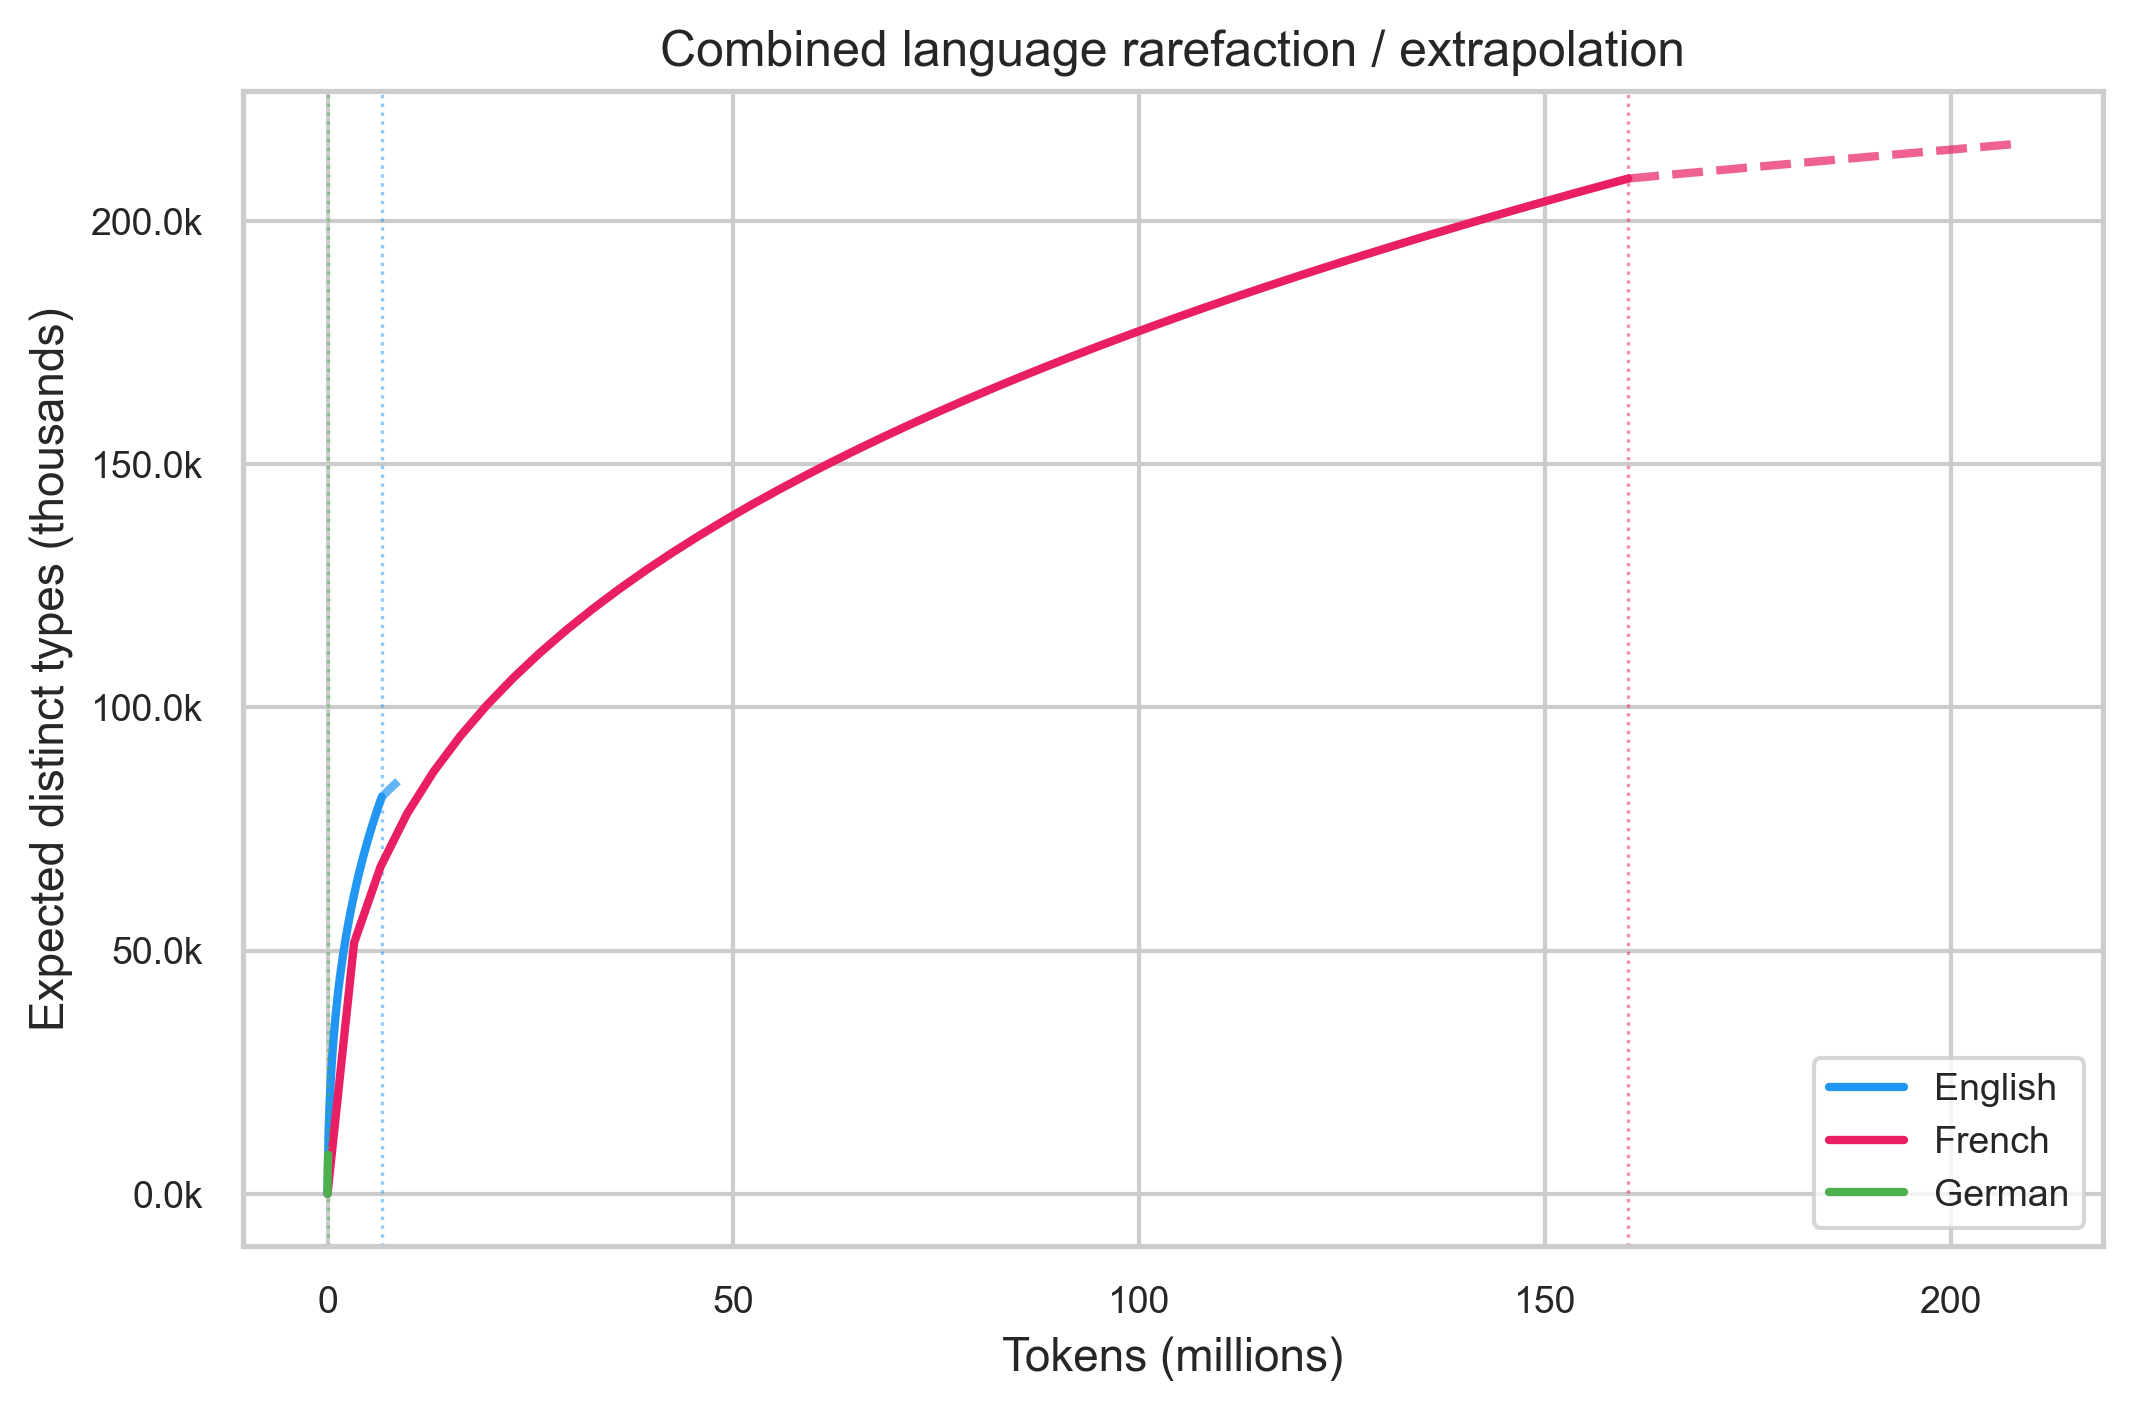
\includegraphics[width=\textwidth]{../results/figures/rarefaction_language_combined.png}
    \caption{Combined language-level rarefaction and extrapolation curves for the spoken/dialogue corpora.}
    \label{fig:results_rarefaction_language_combined}
\end{figure}

\paragraph{Interpretation placeholder.}
TODO: Explain how the combined language curves compare, while noting the effect of unequal corpus sizes.

\subsection{Cross-language comparison}

This comparison uses only spoken and dialogue-based corpora. Shakespeare is excluded here because it is a written literary corpus and serves only as the replication baseline in the first results subsection.

\begin{table}[htbp]
    \centering
    \resizebox{\textwidth}{!}{
    \begin{tabular}{llrrrrr}
        Language & Estimator & Median $S_{\mathrm{obs}}$ & Median $\hat{S}$ & Median $\hat{f}_0$ & Median coverage & Median $\hat{S}/S_{\mathrm{obs}}$ \\
        \hline
        English & Chao1 & 357.0 & 885.9 & 520.1 & 0.7194 & 2.3519 \\
        English & iChao1 & 357.0 & 968.4 & 605.8 & 0.7194 & 2.5719 \\
        English & ACE & 357.0 & 1523.0 & 1161.7 & 0.7194 & 4.0940 \\
        English & Jackknife1 & 357.0 & 585.6 & 228.2 & 0.7194 & 1.6352 \\
        English & Jackknife2 & 357.0 & 764.7 & 405.9 & 0.7194 & 2.1257 \\
        English & Breakaway & 357.0 & 1927.2 & 1554.4 & 0.7194 & 5.2128 \\
        French & Chao1 & 585.0 & 1377.2 & 797.9 & 0.8210 & 2.1066 \\
        French & iChao1 & 585.0 & 1507.5 & 929.2 & 0.8210 & 2.3069 \\
        French & ACE & 585.0 & 2443.5 & 1855.0 & 0.8210 & 3.8163 \\
        French & Jackknife1 & 585.0 & 928.8 & 342.8 & 0.8210 & 1.5676 \\
        French & Jackknife2 & 585.0 & 1200.7 & 614.5 & 0.8210 & 2.0035 \\
        French & Breakaway & 585.0 & 3249.9 & 2611.2 & 0.8210 & 4.9321 \\
        German & Chao1 & 543.0 & 1269.4 & 739.4 & 0.7838 & 2.2451 \\
        German & iChao1 & 543.0 & 1359.3 & 831.2 & 0.7838 & 2.4446 \\
        German & ACE & 543.0 & 2188.3 & 1645.3 & 0.7838 & 4.0295 \\
        German & Jackknife1 & 543.0 & 855.8 & 312.8 & 0.7838 & 1.6027 \\
        German & Jackknife2 & 543.0 & 1111.3 & 568.3 & 0.7838 & 2.0642 \\
        German & Breakaway & 543.0 & 2500.3 & 1940.1 & 0.7838 & 5.2887 \\
    \end{tabular}}
    \caption{Cross-language estimator summary for spoken/dialogue corpora only. Shakespeare is excluded.}
    \label{tab:results_cross_language_estimator_summary}
\end{table}

\paragraph{Table interpretation placeholder.}
TODO: Explain the cross-language table while being careful about sample-size and corpus-composition differences.

\begin{figure}[htbp]
    \centering
    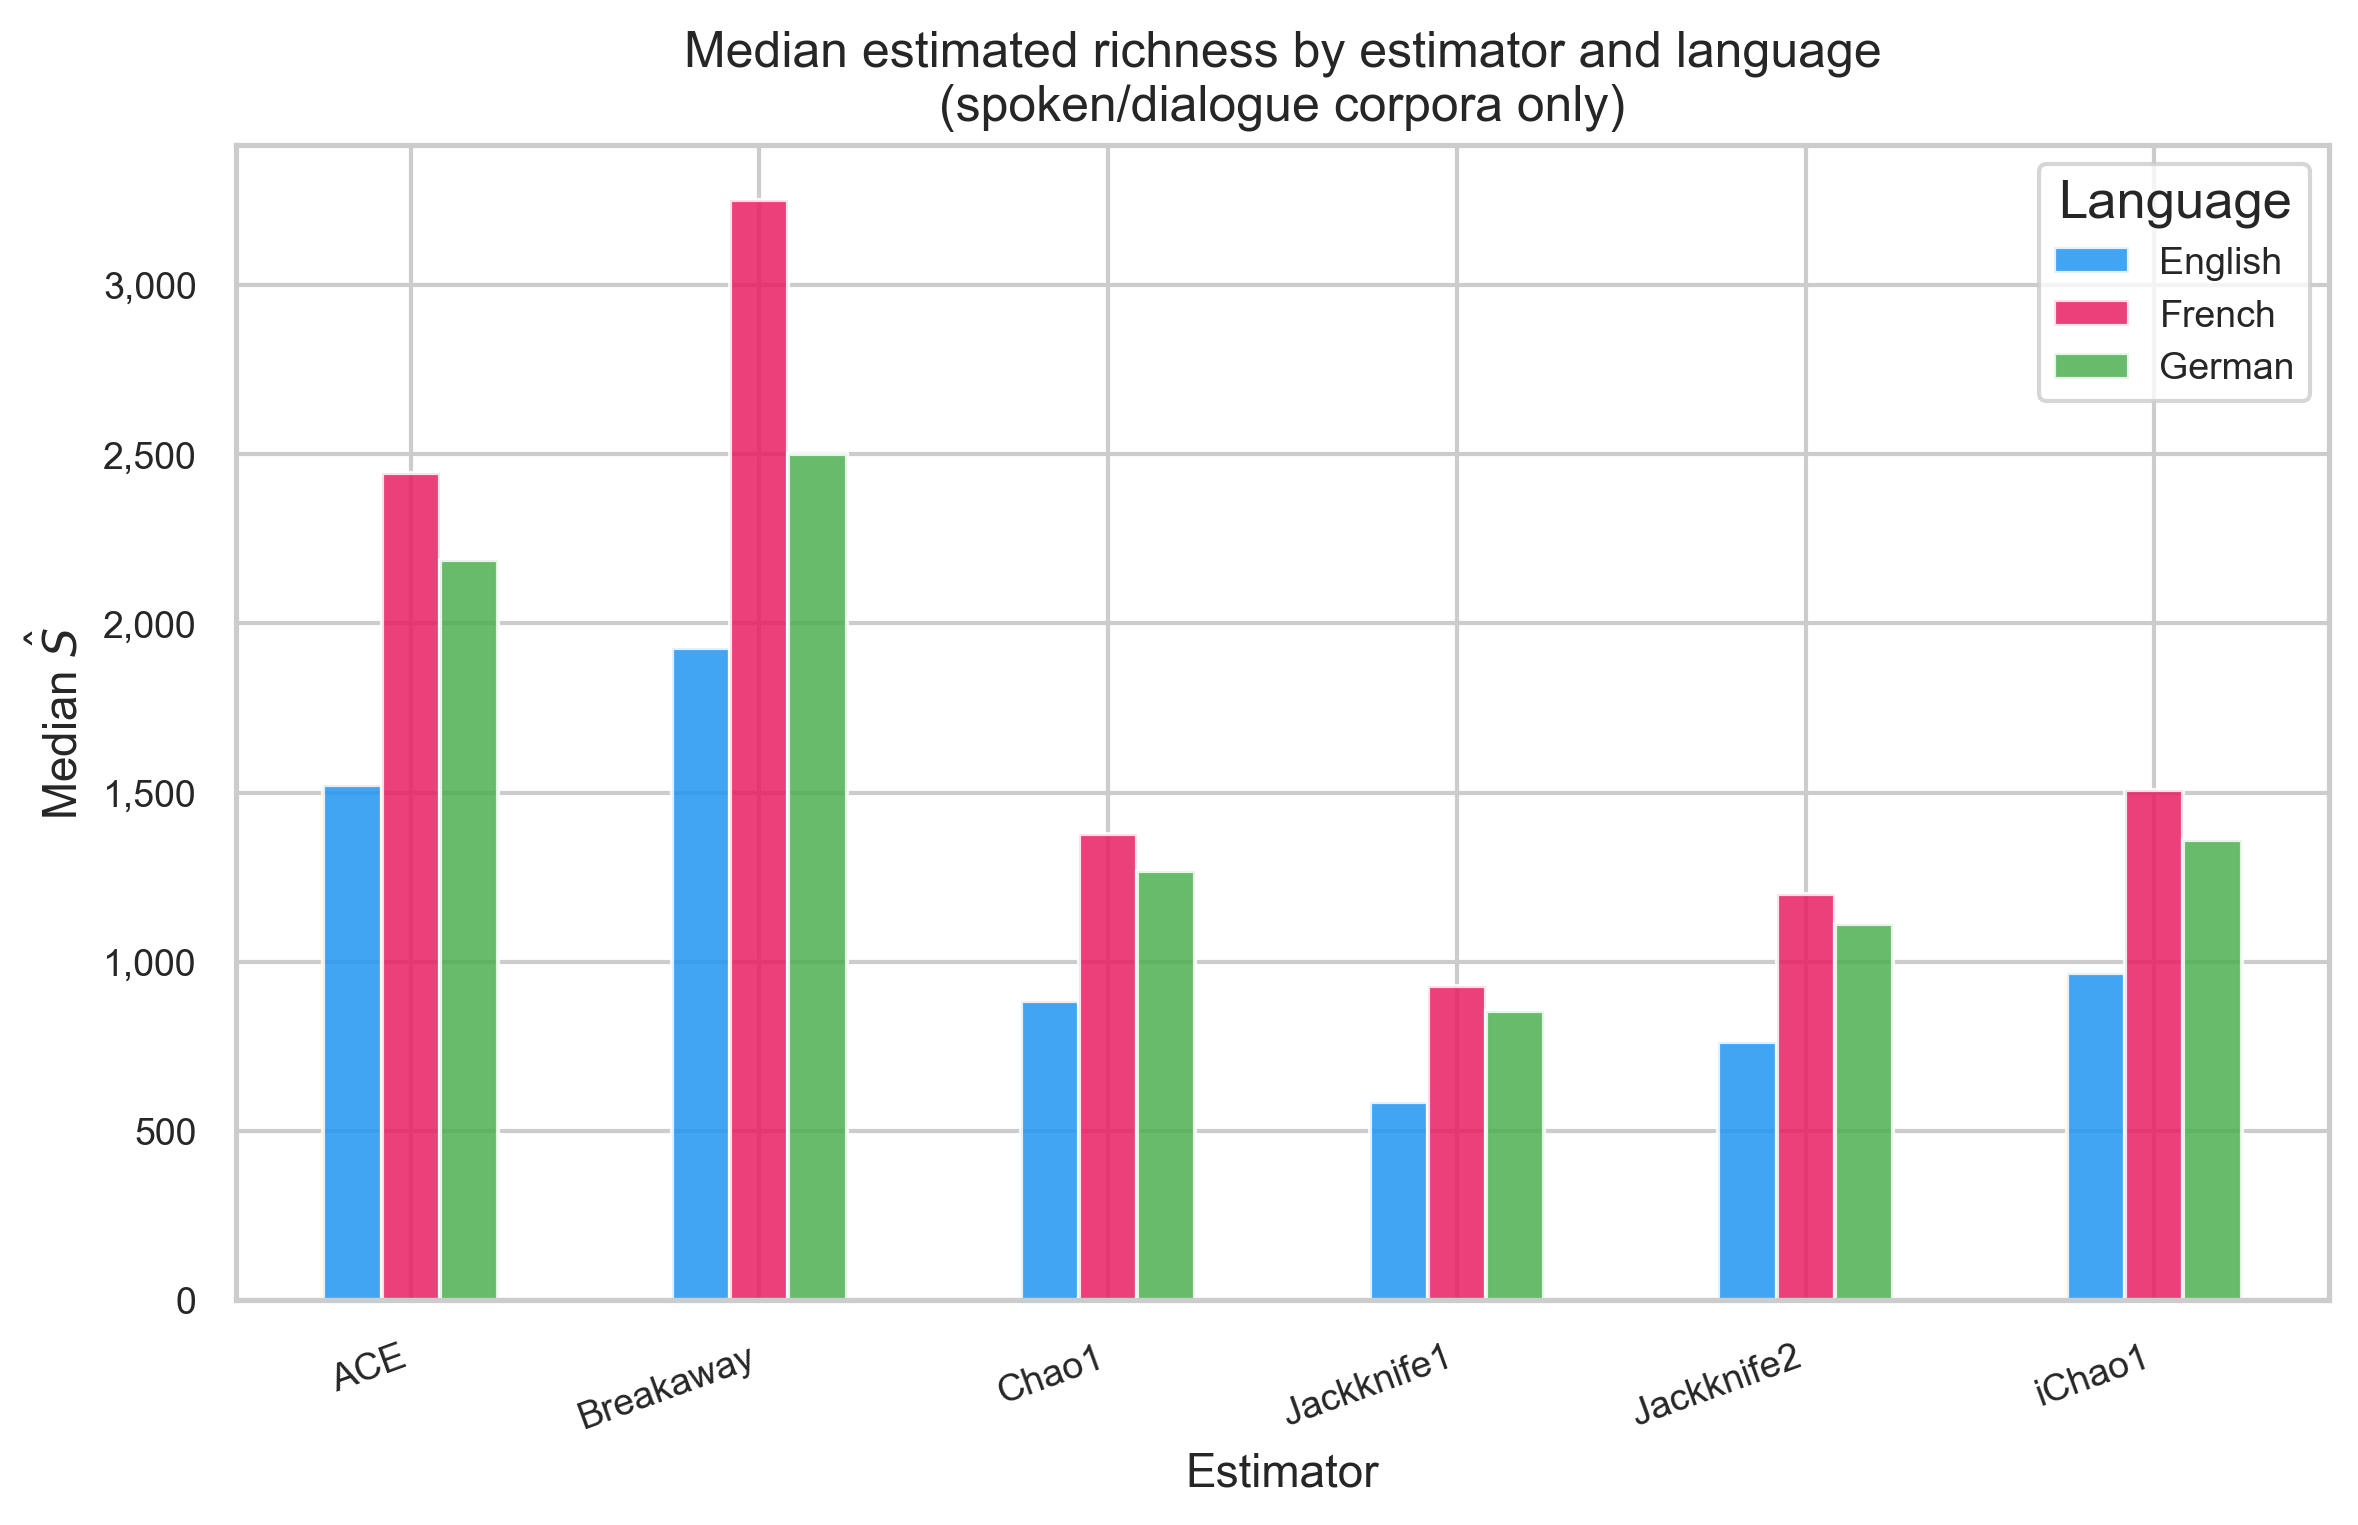
\includegraphics[width=\textwidth]{../results/figures/cross_language_median_Shat.png}
    \caption{Median estimated richness by language and estimator for the spoken/dialogue corpora.}
    \label{fig:results_cross_language_median_shat}
\end{figure}

\paragraph{Interpretation placeholder.}
TODO: Explain the main cross-language differences and whether they appear consistent across estimators.

\begin{figure}[htbp]
    \centering
    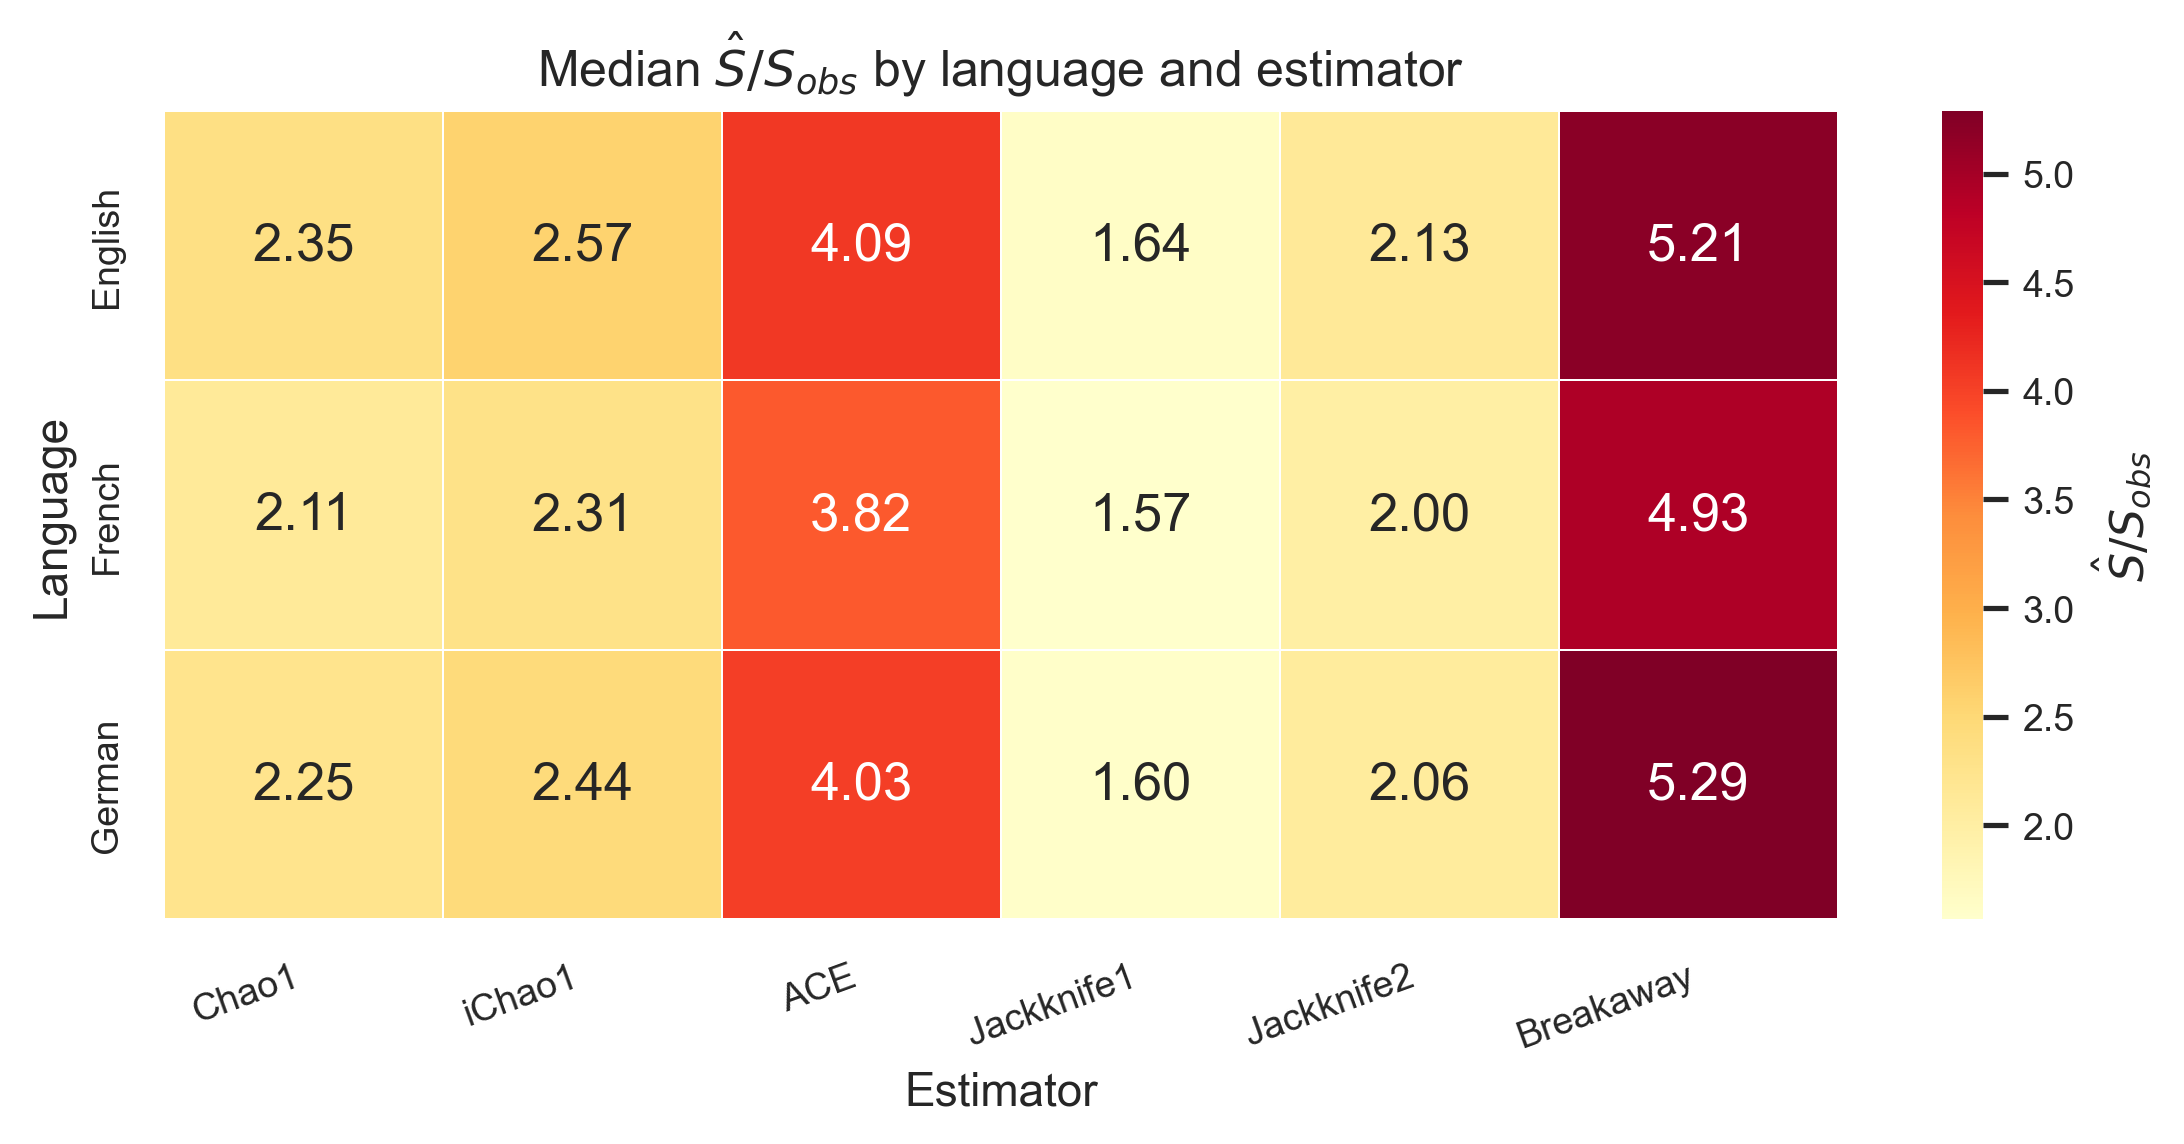
\includegraphics[width=\textwidth]{../results/figures/coverage_standardized_language_comparison.png}
    \caption{Median estimated-to-observed richness ratio by language and estimator.}
    \label{fig:results_coverage_standardized_language_comparison}
\end{figure}

\paragraph{Interpretation placeholder.}
TODO: Explain how the ratio comparison changes the interpretation relative to raw estimated richness.

\begin{figure}[htbp]
    \centering
    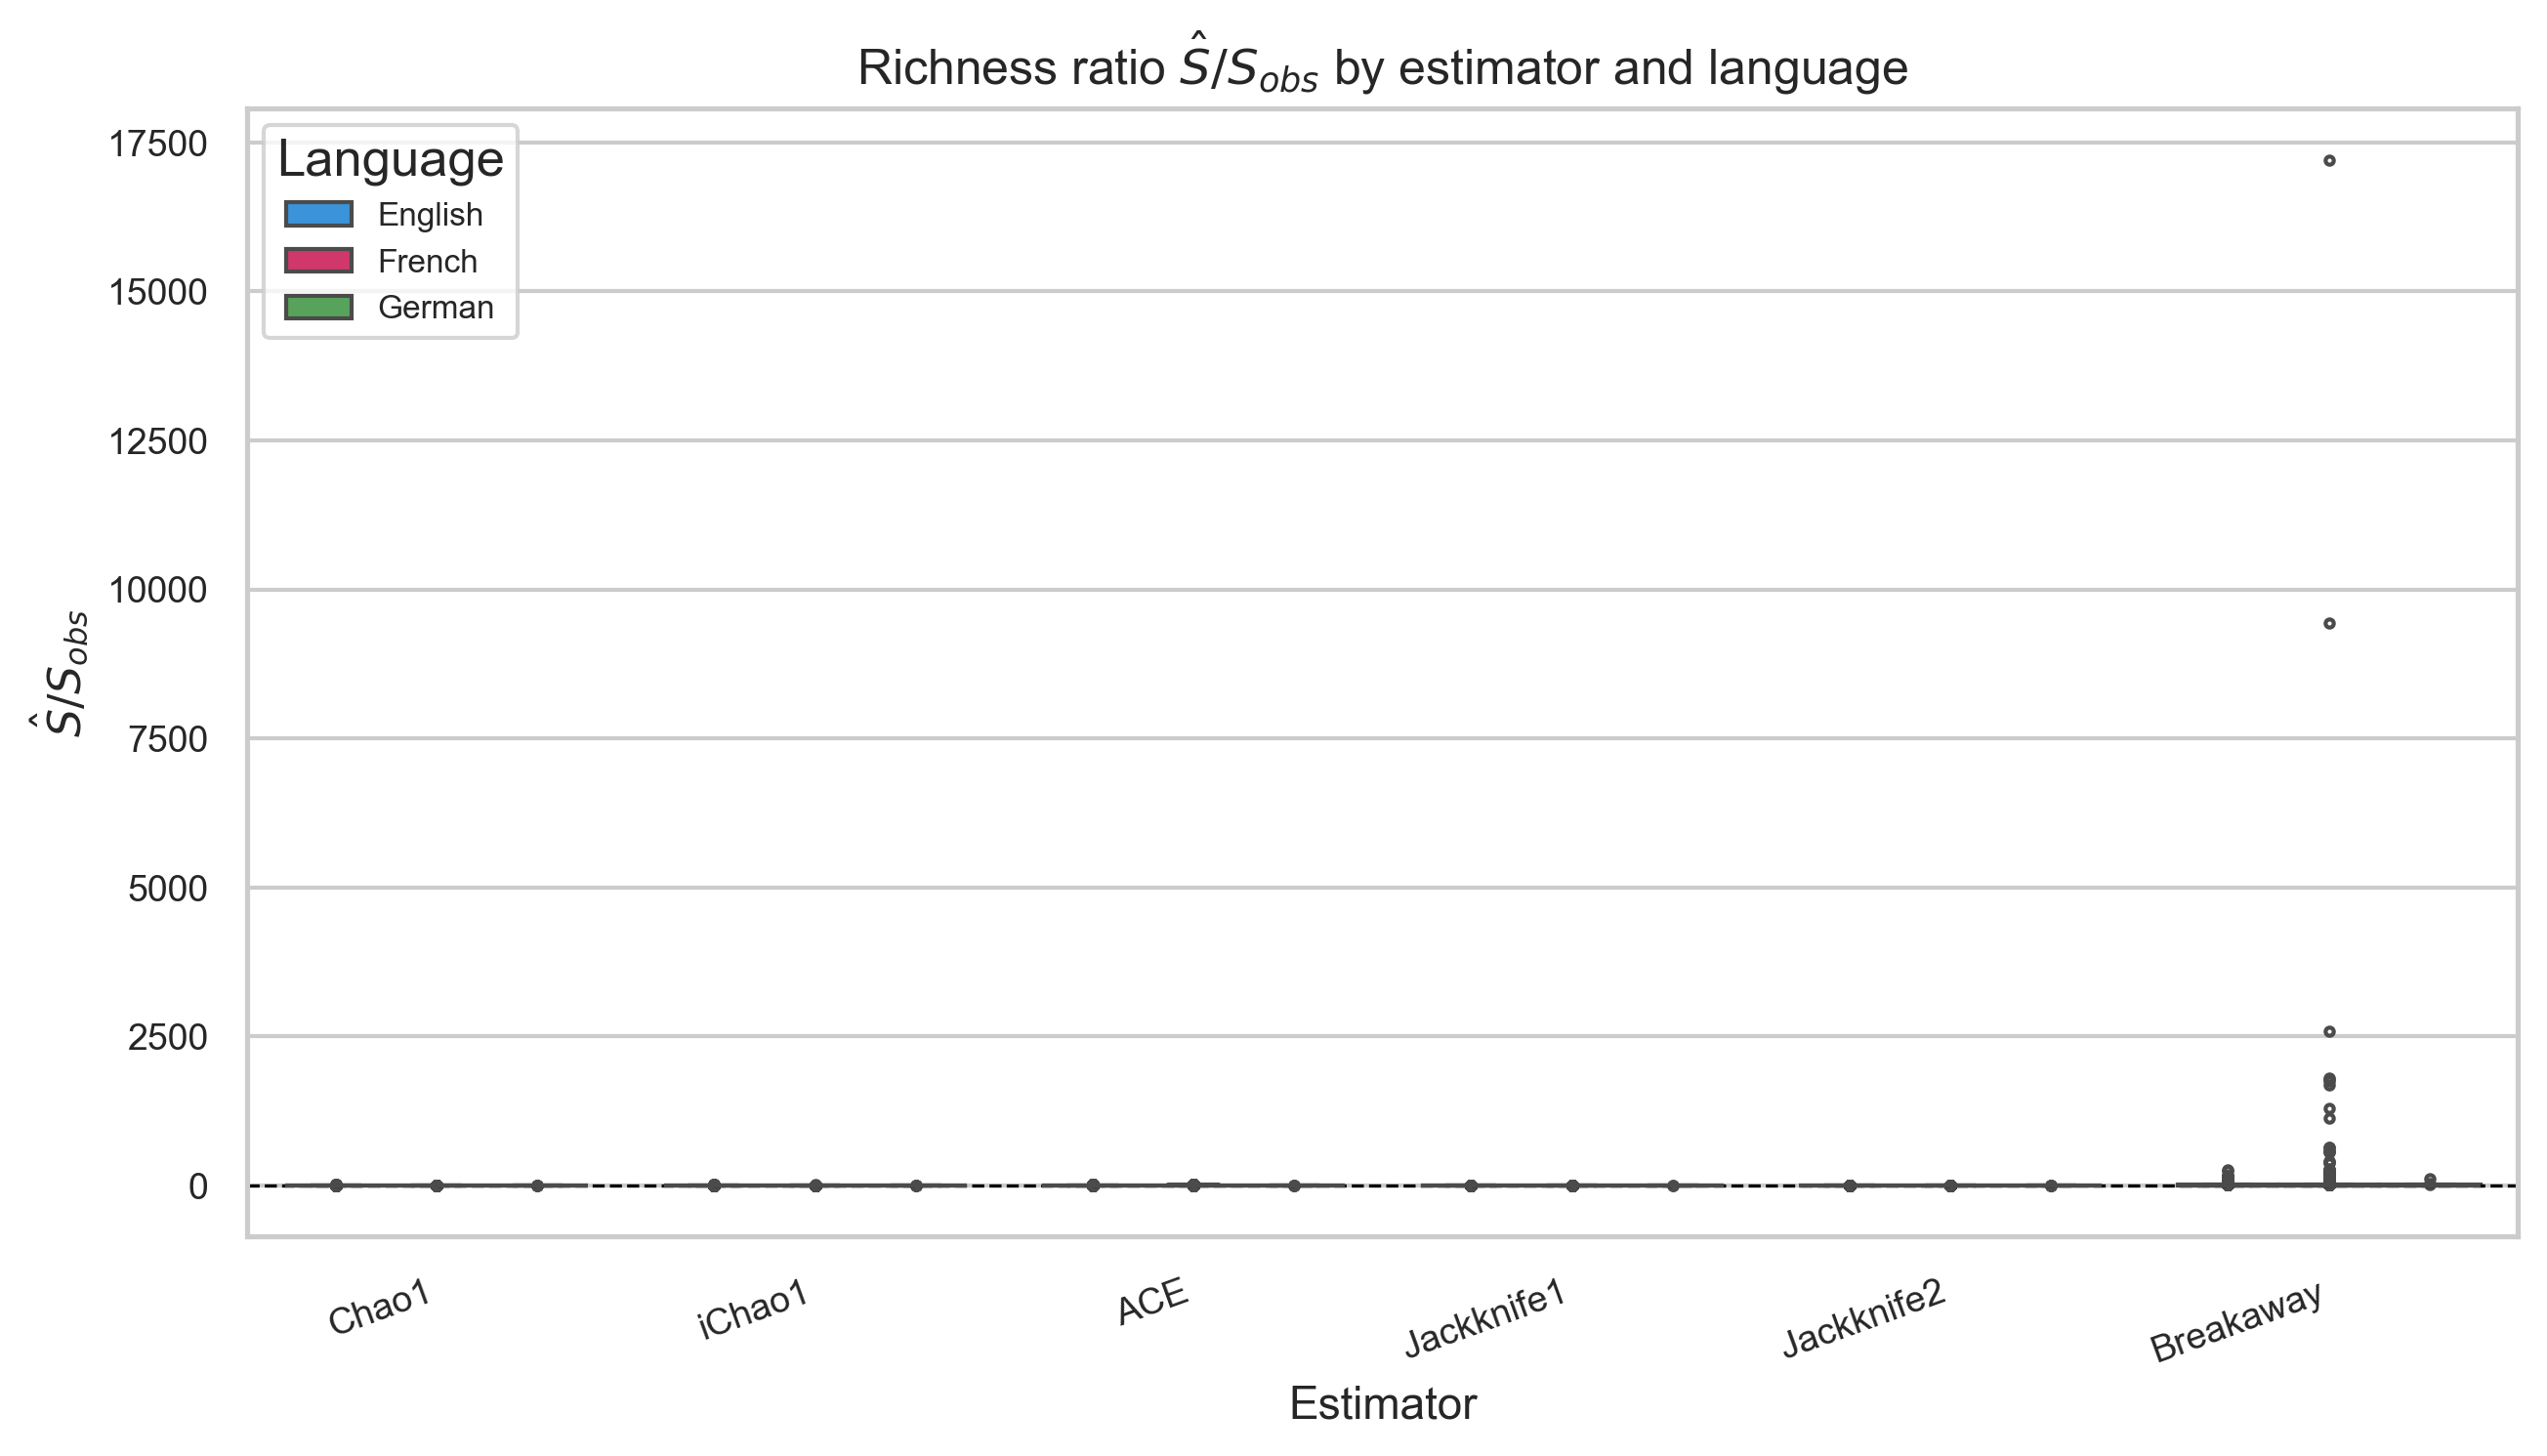
\includegraphics[width=\textwidth]{../results/figures/cross_language_ratio_boxplot.png}
    \caption{Distribution of estimated-to-observed richness ratios by estimator and language.}
    \label{fig:results_cross_language_ratio_boxplot}
\end{figure}

\paragraph{Interpretation placeholder.}
TODO: Explain which language-estimator combinations require the largest extrapolation beyond the observed vocabulary.

\subsection{Estimator agreement and disagreement}

Finally, we compare the estimators directly across all spoken/dialogue corpora.

\begin{table}[htbp]
    \centering
    \resizebox{\textwidth}{!}{
    \begin{tabular}{lrrrrl}
        Estimator & Mean ratio & Median ratio & IQR & Failure rate & Typical behavior \\
        \hline
        Chao1 & 2.2673 & 2.2119 & 0.7028 & 0.0 & Lower bound via $f_1/f_2$ ratio \\
        iChao1 & 2.4760 & 2.4246 & 0.7789 & 0.0 & Tighter lower bound using $f_3/f_4$ \\
        ACE & 3.9731 & 3.9421 & 0.9818 & 0.1 & Heterogeneity-corrected lower bound \\
        Jackknife1 & 1.5790 & 1.5998 & 0.1413 & 0.0 & Delete-one jackknife \\
        Jackknife2 & 2.0236 & 2.0624 & 0.2837 & 0.0 & Delete-two jackknife \\
        Breakaway & 13.6129 & 5.0446 & 3.8501 & 50.7 & Ratio-regression; unstable for small $n$ \\
    \end{tabular}}
    \caption{Global estimator behavior across all spoken/dialogue corpora. Ratios are $\hat{S}/S_{\mathrm{obs}}$.}
    \label{tab:results_estimator_summary_global}
\end{table}

\paragraph{Table interpretation placeholder.}
TODO: Explain the global estimator behavior table, especially the contrast between stable lower-bound estimators and Breakaway.

\begin{table}[htbp]
    \centering
    \begin{tabular}{lrrr}
        Estimator & Total units & Failed/undefined & Failure rate (\%) \\
        \hline
        Chao1 & 16374 & 0 & 0.0 \\
        iChao1 & 16374 & 0 & 0.0 \\
        ACE & 16374 & 10 & 0.1 \\
        Jackknife1 & 16374 & 0 & 0.0 \\
        Jackknife2 & 16374 & 2 & 0.0 \\
        Breakaway & 16374 & 8300 & 50.7 \\
    \end{tabular}
    \caption{Estimator failure and undefined-output summary for spoken/dialogue corpora.}
    \label{tab:results_estimator_failure_summary}
\end{table}

\paragraph{Table interpretation placeholder.}
TODO: Explain which estimators are numerically stable and why failed estimates matter for interpretation.

\begin{figure}[htbp]
    \centering
    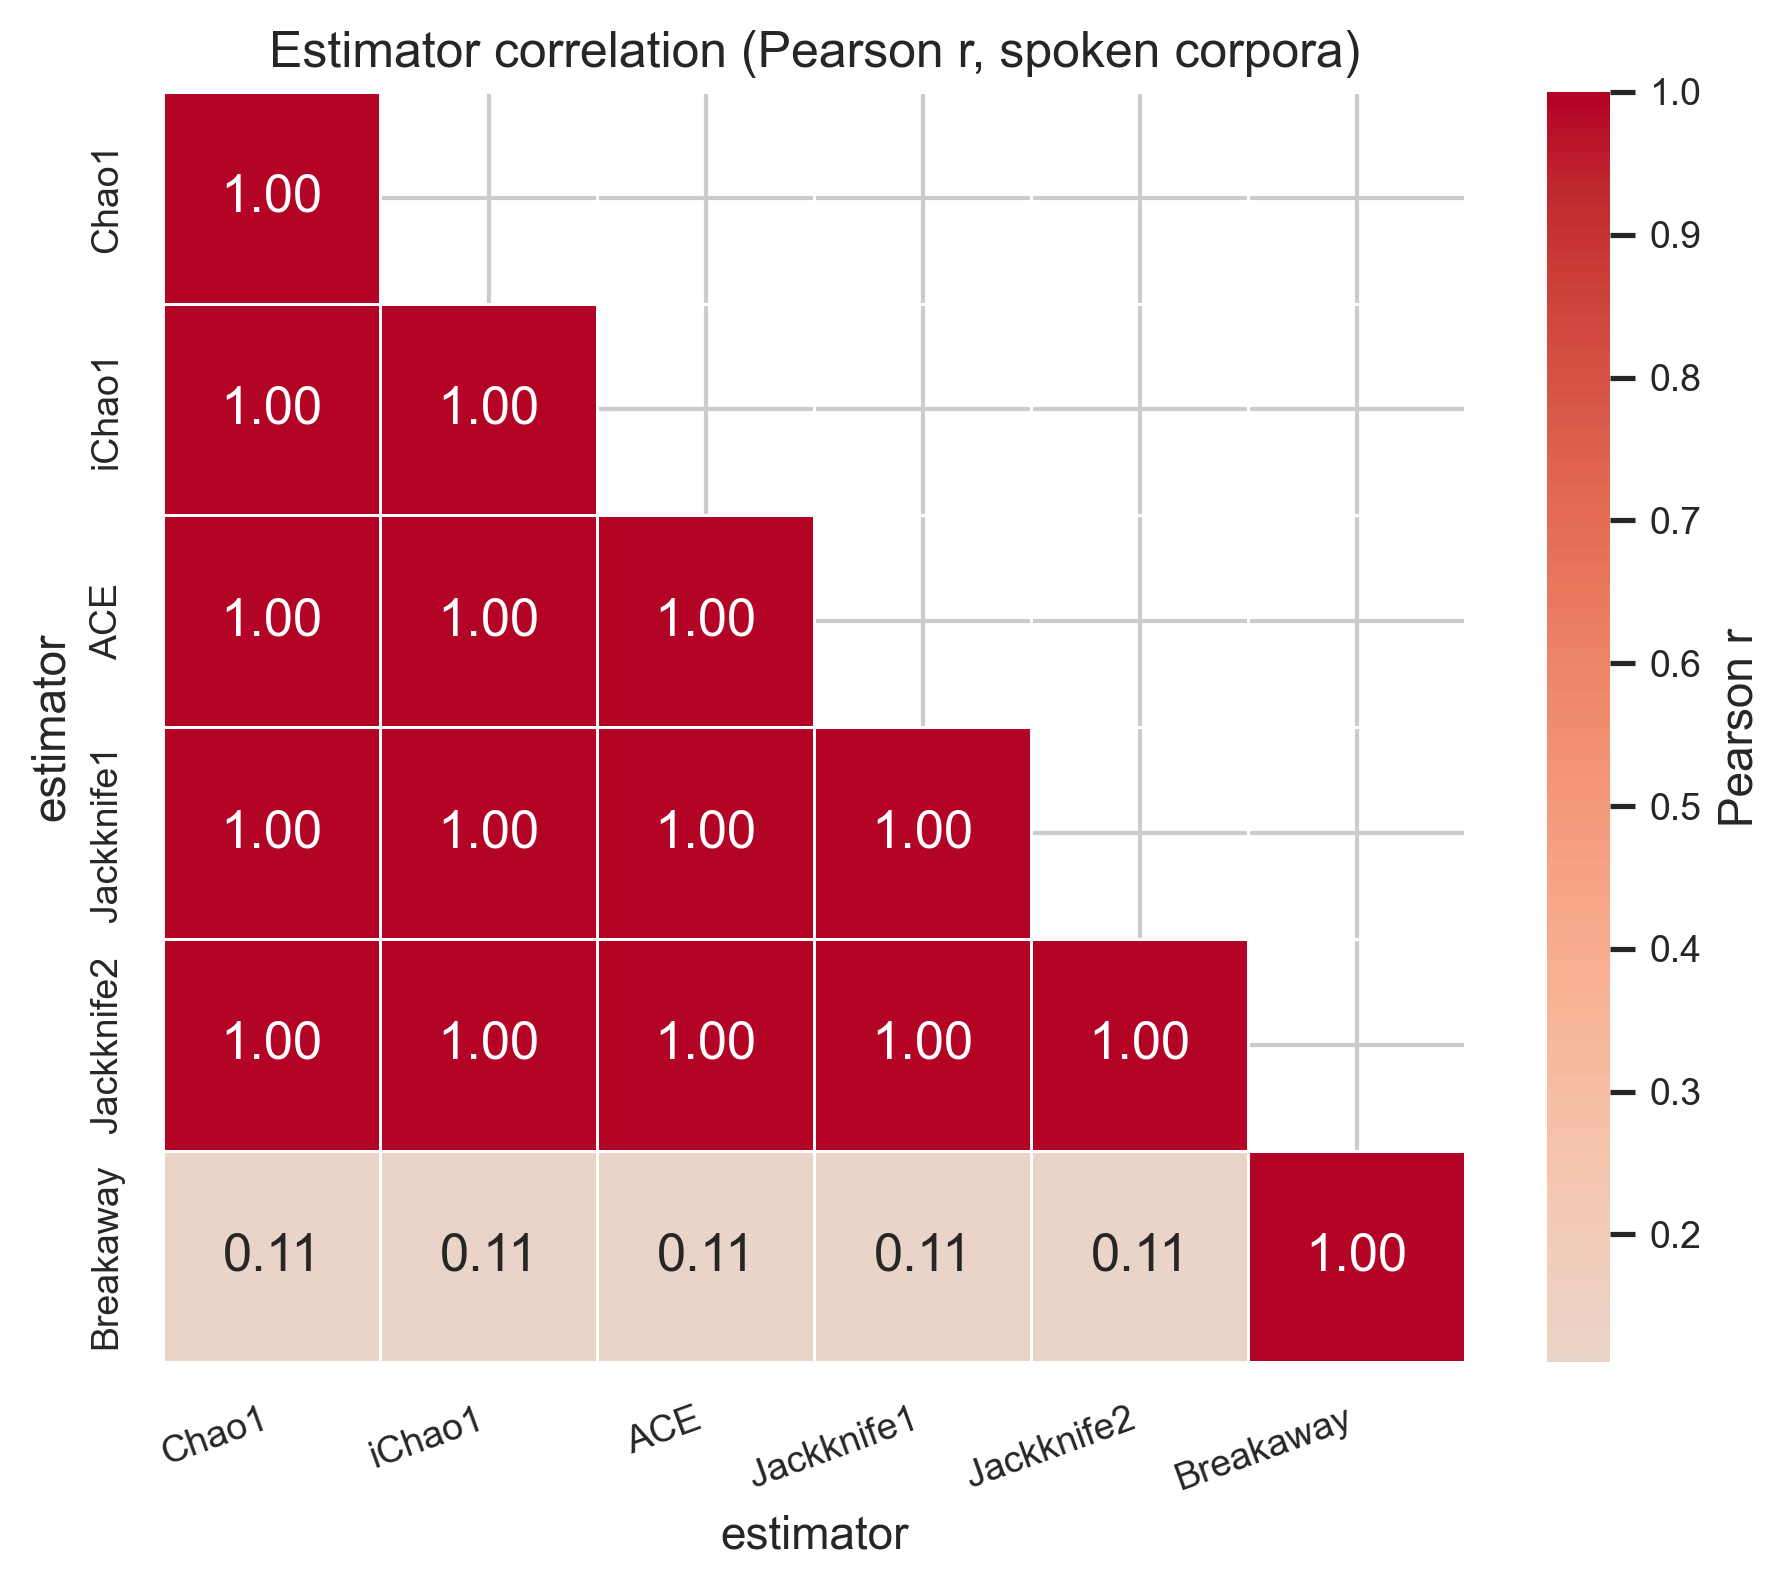
\includegraphics[width=\textwidth]{../results/figures/estimator_correlation_heatmap.png}
    \caption{Correlation between estimator outputs across the spoken/dialogue corpora.}
    \label{fig:results_estimator_correlation_heatmap}
\end{figure}

\paragraph{Interpretation placeholder.}
TODO: Explain which estimators agree most strongly and where disagreement is expected.

\begin{figure}[htbp]
    \centering
    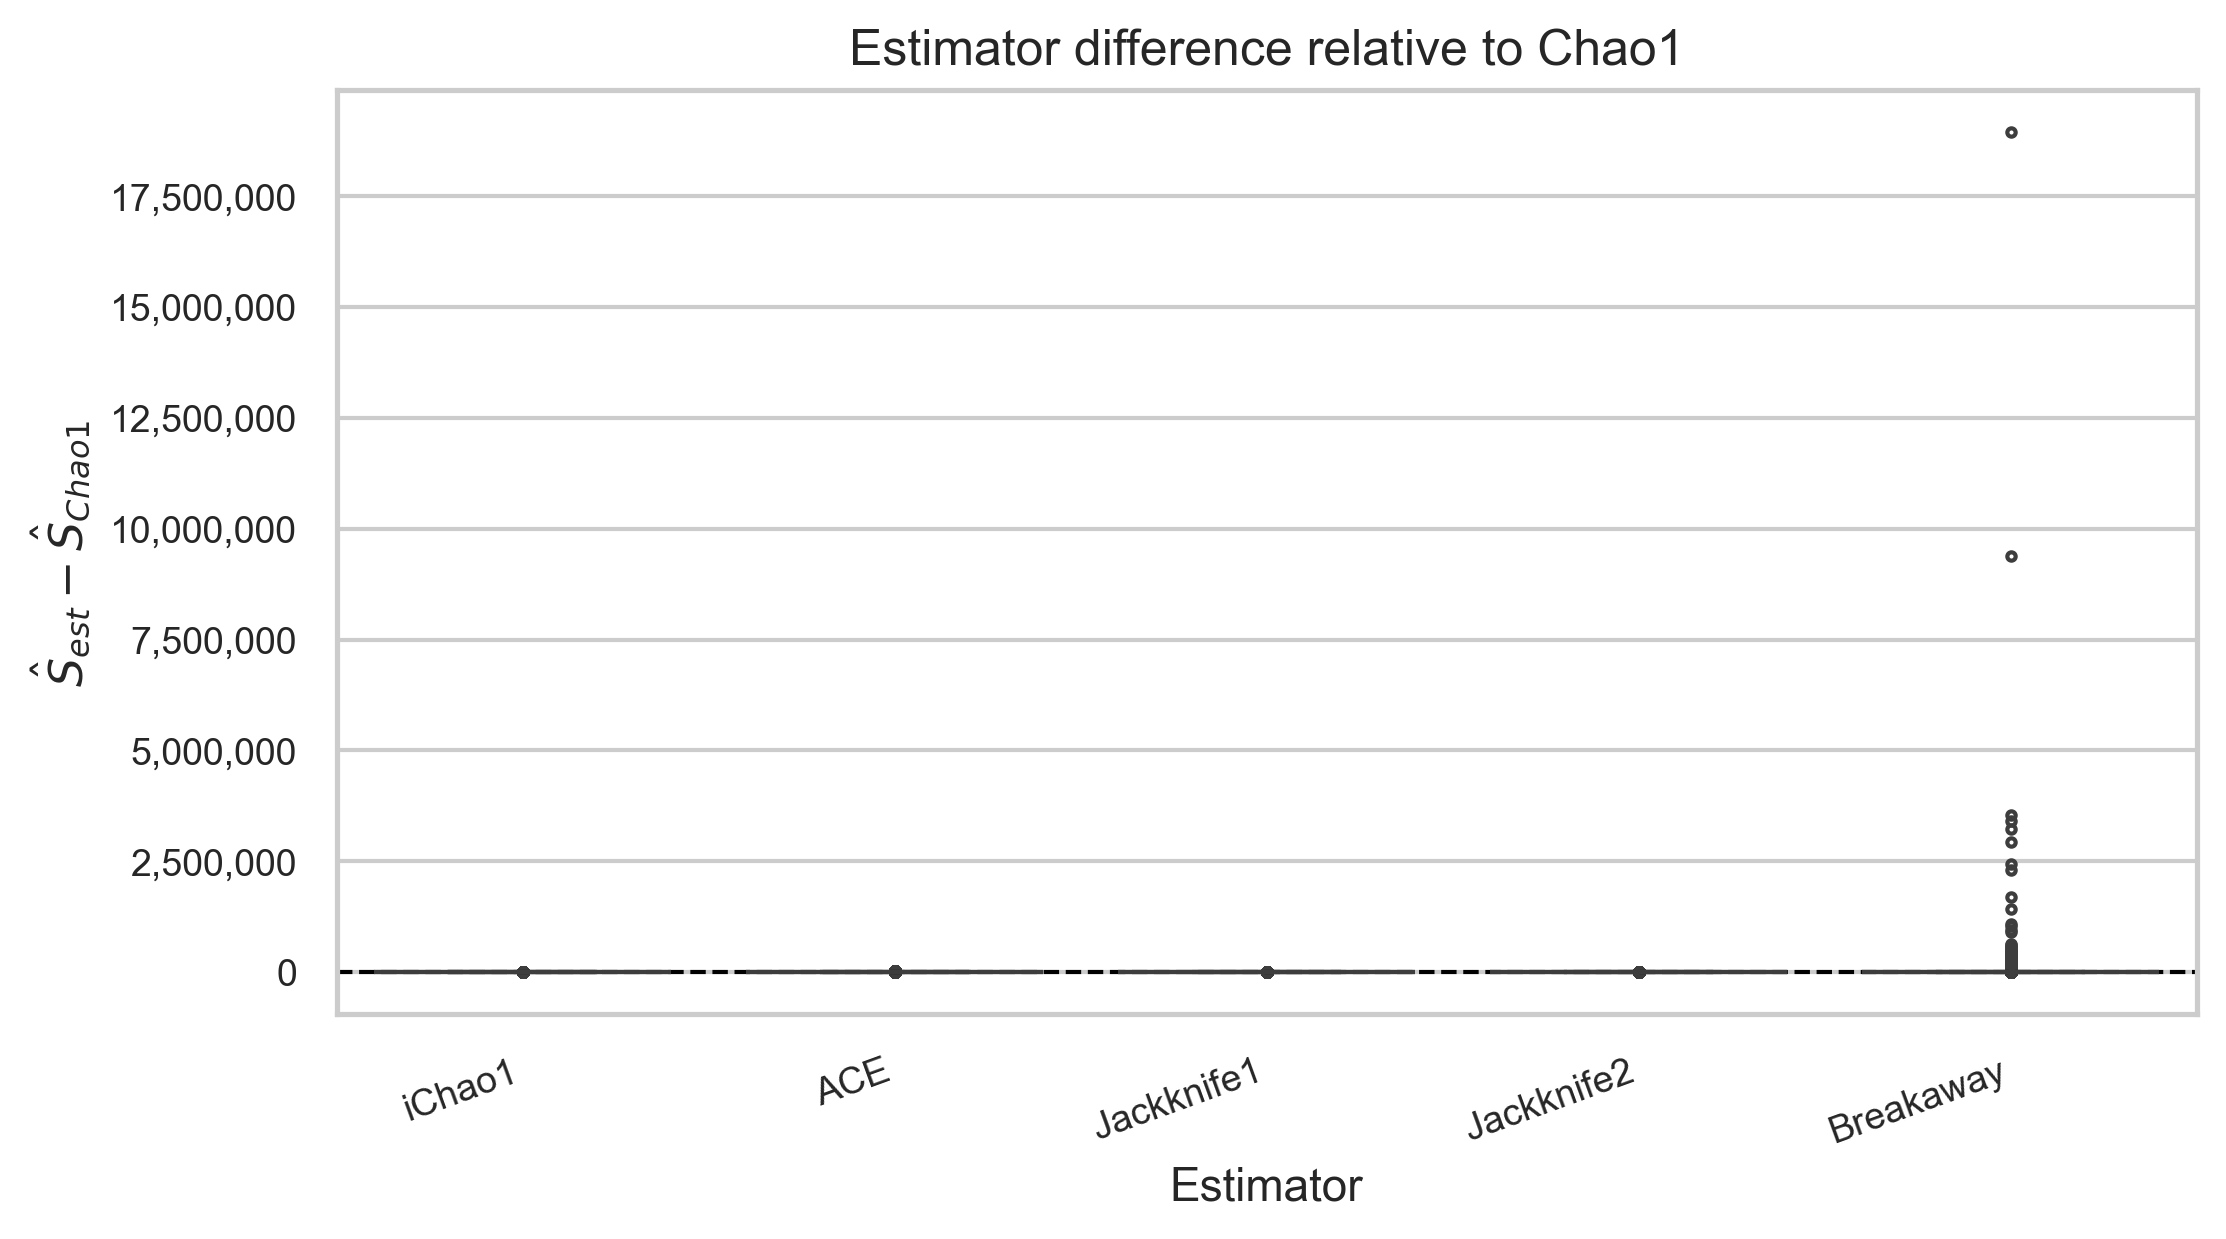
\includegraphics[width=\textwidth]{../results/figures/estimator_ratio_to_chao1.png}
    \caption{Difference between each estimator and Chao1 across the spoken/dialogue corpora.}
    \label{fig:results_estimator_difference_to_chao1}
\end{figure}

\paragraph{Interpretation placeholder.}
TODO: Explain which estimators lie above or below Chao1 and how large the differences are.

\begin{figure}[htbp]
    \centering
    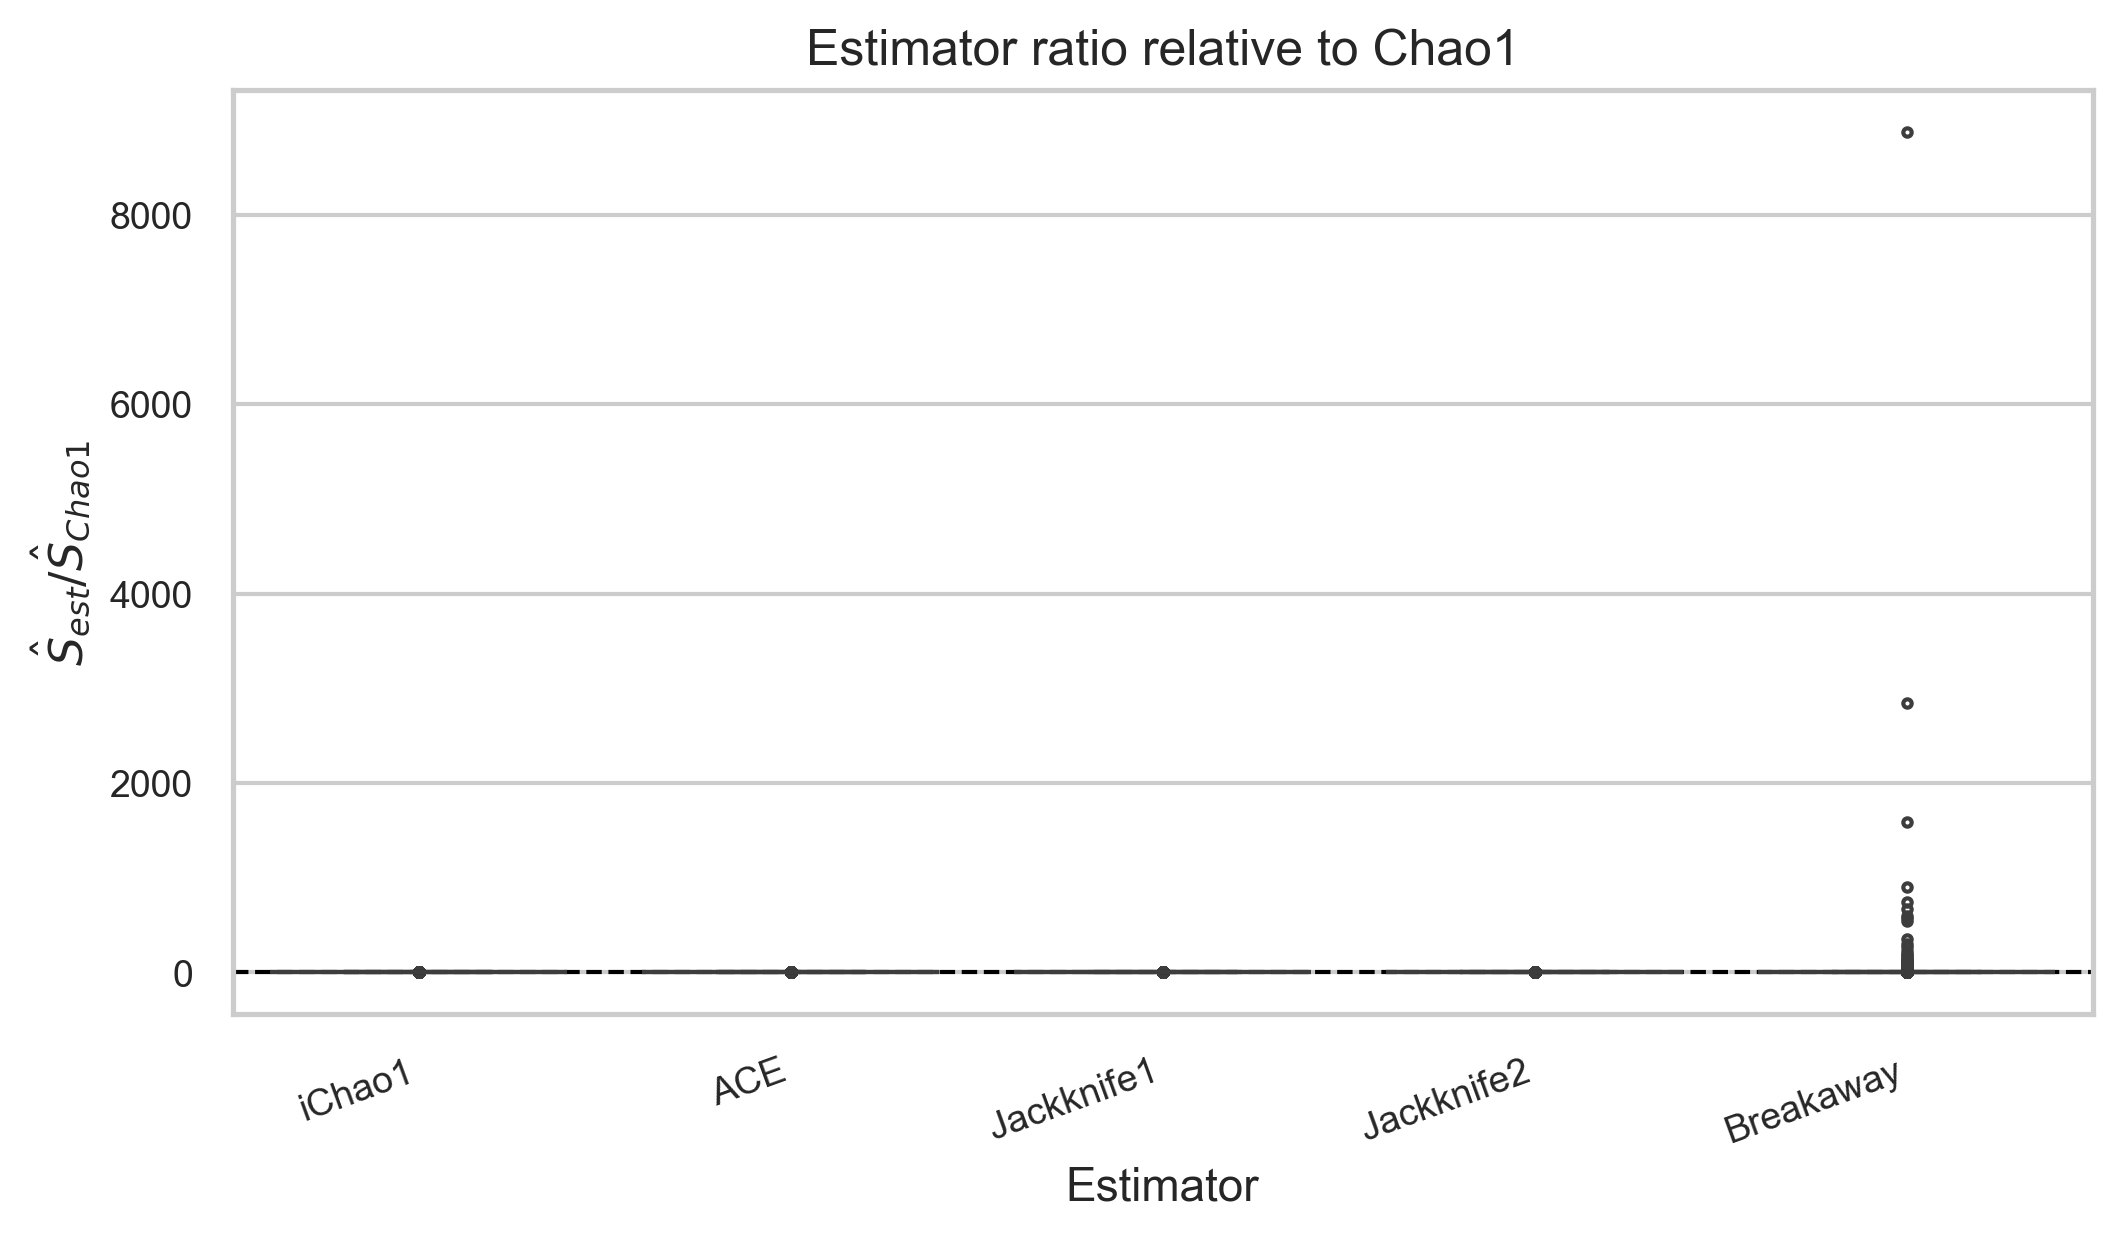
\includegraphics[width=\textwidth]{../results/figures/estimator_ratio_over_chao1.png}
    \caption{Ratio between each estimator and Chao1 across the spoken/dialogue corpora.}
    \label{fig:results_estimator_ratio_over_chao1}
\end{figure}

\paragraph{Interpretation placeholder.}
TODO: Explain the relative scale of the estimator differences using Chao1 as a baseline.

\section{Discussion}\label{sec:discussion}

\section{Conclusion}\label{sec:conclusion}

Summarize findings, answer research questions, suggest future work.

% --- after your conclusion section, before \bibliographystyle / \bibliography ---

\appendix

\section{Parametric mixture models}\label{app:parametric_models}

We give the full probability mass functions for the three parametric Poisson mixture models fitted in Section~\ref{sec:mixture_models}. In each case, the conditional model is $X \mid \Lambda = \lambda \sim \mathrm{Poisson}(\lambda)$; the models differ only in the mixing distribution assumed for $\Lambda$.

\textbf{Gamma--Poisson mixture (Negative Binomial).}\;
Assume $\Lambda \sim \mathrm{Gamma}(r,\, r/\mu)$.
Integrating out $\Lambda$ yields the negative binomial distribution
\[
p(x;\,r,\mu)
= \frac{\Gamma(r+x)}{\Gamma(r)\,x!}
  \left(\frac{r}{r+\mu}\right)^{\!r}
  \left(\frac{\mu}{r+\mu}\right)^{\!x},
\qquad x \in \mathbb{N}_0.
\]
This is a classical two-parameter family introduced by
Fisher et al.~\cite{fisher1943} for modelling species abundances.

\textbf{LogNormal--Poisson mixture.}\;
Assume $\log\Lambda \sim \mathcal{N}(\mu,\sigma^2)$.
The marginal distribution has no closed form and is given by
\[
p(x;\,\mu,\sigma)
= \int_0^\infty
  \frac{\lambda^x\, e^{-\lambda}}{x!}\;
  \frac{1}{\lambda\,\sigma\sqrt{2\pi}}
  \exp\!\left(-\frac{(\log\lambda - \mu)^2}{2\sigma^2}\right)
  d\lambda,
\qquad x \in \mathbb{N}_0.
\]
The integral must be evaluated numerically.


\textbf{Poisson--Inverse Gaussian mixture.}
Assume $\Lambda \sim \mathrm{InvGaussian}(\mu,\phi)$.
The marginal distribution is
\[
p(x;\,\mu,\phi)
= \int_0^\infty
  \frac{\lambda^x\, e^{-\lambda}}{x!}\;
  dG_{\mathrm{IG}}(\lambda),
\qquad x \in \mathbb{N}_0,
\]
where $G_{\mathrm{IG}}$ denotes the inverse Gaussian CDF. The
probabilities can be computed exactly from the Taylor coefficients of
the probability generating function
\[
G(z)
= \exp\!\left(
  \frac{\phi}{\mu}
  \left(1 - \sqrt{1 + \frac{2\mu^2(1-z)}{\phi}}\right)
\right).
\]

\section{Data Sources}\label{app:sources}
\begin{itemize}
    \item \textbf{British National Corpus (BNC)}\\
    \url{https://www.english-corpora.org/bnc/}

    \item \textbf{Santa Barbara Corpus of Spoken American English}\\
    \url{https://www.linguistics.ucsb.edu/research/santa-barbara-corpus-spoken-american-english}

    \item \textbf{Corpus of Contemporary American English (COCA), Spoken Component}\\
    \url{https://www.english-corpora.org/coca-spoken.asp}

    \item  \textbf{A collection of transcripts of real French dialogues from various sources, including parliamentary proceedings, interviews, debates, meetings, and free conversations. }
    \url{https://huggingface.co/datasets/OpenLLM-France/Claire-Dialogue-French-0.1}
\end{itemize}

\clearpage
\bibliographystyle{plain}
\bibliography{references}
\end{document}
